\documentclass[reprint,amsmath,amssymb,aps,pre,showkeys,showpacs,nofootinbib]{revtex4-1}
% Latex
\usepackage[english]{babel}
\usepackage[utf8]{inputenc}
\usepackage[T1]{fontenc}
% Xelatex
%\usepackage{polyglossia}
%\usepackage{fontspec}
%\setdefaultlanguage{english}
%\setmainfont{DejaVu Sans}
%\setsansfont{DejaVu Sans}
%\setmonofont{DejaVu Sans Mono}
\usepackage{bm}
\usepackage{cleveref}
\usepackage{xcolor}
\usepackage{algpseudocode}
\usepackage{graphicx}
\usepackage{subfigure}

\newtheorem{definition}{Definition}

\definecolor{light-gray}{gray}{0.95}
\newcommand{\code}[1]{\colorbox{light-gray}{\texttt{#1}}}
% When cleveref fails to do its job
\newcommand{\apref}[1]{Appendix \ref{#1}}

\begin{document}
\preprint{APS/123-QED}

\author{Aleksei Samarin\textsuperscript{1,2}}
\author{Vasily Postnicov\textsuperscript{1}}
\author{Marina Karsanina\textsuperscript{1}}
\author{Efim Lavrukhin\textsuperscript{1,2}}
\author{Dina Gafurova\textsuperscript{3}}
\author{Aleksey Khlyupin\textsuperscript{1}}
\author{Kirill Gerke\textsuperscript{1}}
\email{kg@ifz.ru}

\affiliation{\textsuperscript{1}Schmidt Institute of Physics of the Earth of
  Russian Academy of Sciences, Moscow, 107031, Russia}
\affiliation{\textsuperscript{2}Computational Mathematics and Cybernetics,
  Lomonosov Moscow State University, Moscow, 119991, Russia}
\affiliation{\textsuperscript{3}Oil and Gas Research Institute Russian Academy
  of Sciences (OGRI RAS) 3, Gubkina st., Moscow, 119333, Russian Federation}

\title{Evaluation of classical correlation functions from 2/3D images on CPU and
  GPU architectures: introducing CorrelationFunctions.jl}

\begin{abstract}
  What have we done?
\end{abstract}

\maketitle

\section{Background and motivation}
\label{sec:background}
Materials are ubiquitous both in nature and in industrial human activities, and
their physical properties are interconnected to
structure\cite{Torquato_book}\cite{Sahimi_book}\cite{Adler_recon}. The information
about the structure usually comes in the way of 2D and 3D images obtained by
microscopy, tomography and other related methodologies. This structural
information can be used for numerous types of analysis, including simulations of
different processes within studied materials or evaluation of their properties
using so-called pore-scale modelling. Unlike computational modelling techniques
a whole class of approximate methods exists including (rigorous) bounds that
allows very fast estimations of physical properties albeit the bounds themselves
are too wide to be applicable in majority of practical problems. Nonetheless, it
is noteworthy that such bounds are originally based on structural descriptors in
the form of correlation functions.

Two ways exist to obtain correlation functions for a given structure at hand:
measure them either experimentally with the help of scattering intensity or
from digital images. None is perfect, as the first approach suffers from the
limitation of CFs that can be obtained this way, while the second one provides
information with limited resolution or/and resolution to field-of-view ratio. In
addition to the resolution conundrum, the most useful imaging methods such as
X-ray computed tomography (XCT) and scanning electron microscopy (SEM) provide
gray-scale images (e.g., X-ray attenuation or electron back-scattering
distributions) due to their underlying physical principles and require labeling
of constituent phases (this is called segmentation) before computation of
CFs. If properly segmented, high-resolution digital images do provide a
possibility to compute any correlation function and, thus, possibility to
address numerous fundamental and practical research problems.

Correlation functions (CFs) as invaluable universal descriptors of structure are
utilized in a multitude of scientific disciplines: material sciences, rock
physics, soil physics and hydrology, cosmology and food engineering, biology and
many others. Computed from 2D and 3D images, CFs can be applied to:
\begin{enumerate}
  \item to characterize the morphology and representativeness via correlation
    lengths;
  \item to perform stochastic reconstructions from experimentally measured CFs
    or 2D to 3D reconstructions based on CFs that can be extracted from less
    dimensions or through penetrable sphere model;
  \item compare different structures to each other, including verification of
    stochastic reconstructions;
  \item compress structural information in the form of raw or parameterized CFs
    with the possibility to recover the structure using stochastic
    reconstruction
  \item describe structural dynamics under different boundary conditions;
  \item extract structural features for deep learning;
  \item fuse multi-scale images and structural information as obtained by
    different methods into a single digital model;
  \item quantify spatial heterogeneity.
\end{enumerate}

Stochastic reconstruction is a separate huge topic, as this approach allows to
solve an inverse problem and recover structure from known set of correlation
functions. This ability for recovery serves as the basis for majority of usages
in the list above. While it is necessary to compute CFs from digital images as a
target set for stochastic reconstructions, they rely more on efficient
recomputations or optimizations, e.g., re-evaluation during simulated
annealing. Such optimizations are not the part of the computational package and
are not considered in this work.

There are different types of correlation functions that in general describe some
probabilities. The main parameter of any correlation function is the number of
points that are utilized to evaluate such a probability. While so-called
$n$-point probability function\cite{Torquato_book} will totally describe any
structure in the limit of $n \rightarrow$ number of voxels/pixels on the image,
computing or storing such a function is not practical. Based on information
content, it was shown that increasing the number of point $n > 2$ only
marginally improves the quality of the structure quantification and these
improvements decay with increasing $n$. For stochastic reconstruction purposes
computation of higher-order statistics will, arguably, not be balanced by
increased number of points, but this is the topic of active research. For
aforementioned reasons, we mainly focus on 2-point statistics, leaving the
possibility to include higher order CFs in the future work. The simplest 2-point
probability function ($S_2$ or autocorrelation) actually arise from small angle
scattering experiments and measures the probability that both ends of line
segment with a given length fall into the same phase. Other types include the
probability of a whole line segment to fall into the phase ($L_2$ function) or
to lie on the interface between phases ($F_{ss}$ function), and mainly originate
from aforementioned bounds on physical properties such as permeability and
elasticity. The general idea of computation of different 2-point CFs is shown in
\cref{fig:functions}. All major details and numerous analytical cases can be
found in seminal work of Torquato \cite{Torquato_book}. To all CFs described in this
book and applicable to digital images we shall refer as to classical correlation
functions.

\begin{figure}[ht]
  \centering
  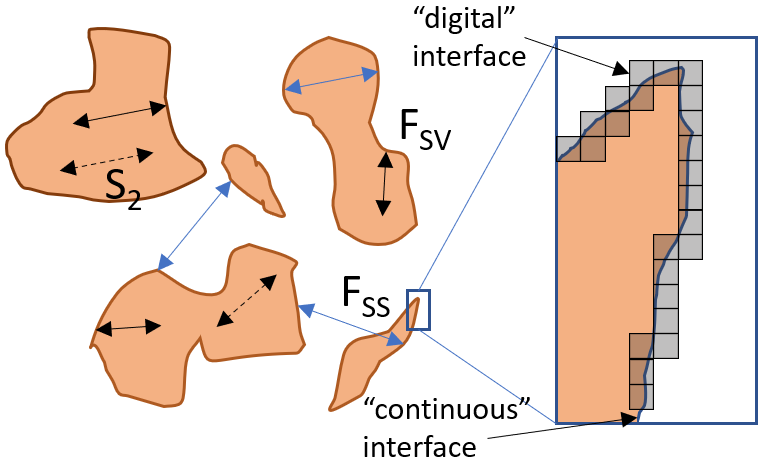
\includegraphics[width=0.9\linewidth]{images/corr.png}
  \caption[]{A schematic depiction of a binary porous media (pores are shown in
    color) with examples of positive events for surface $F_{ss}$, $F_{sv}$ and
    two-point probability $S_2$ correlation functions. The zoomed in area
    represents the difference between the true ``continuous'' interface in
    between pore and solid phases with pixelized ``digital'' interface emerging
    due to limited resolution of digital images.}
  \label{fig:functions}
\end{figure}

While evaluation of correlation functions from 2D and 3D images was a topic of
numerous research papers, the information is highly fragmented, especially in
terms of algorithms and their implementation in the code. Some snippets of code
are available for some functions, but they lack general API and are usually
implemented in proprietary interpreted languages such as Matlab. Due to a recent
leap forward in GPU-based computations, some papers describe computations on
this architecture, but the code is usually not provided. All in all, the
efficient and open-source single API solution utilizing both CPU and GPU
architectures is currently absent.

The aim of this paper is to establish a general open-source solution allowing to
compute all classical correlation functions. This solution should be well
documented with all computational algorithms explained, it should also leverage
on recent advances in programming high-intensity computations and utilize both
CPU and GPU power. Our answer in the form of \code{CorrelationFunctions.jl}
package allows to compute numerous CFs easily on any operating system. The
manuscript describing the package is organized as follows: in \cref{sec:math} we
introduce a reader to the most common and useful correlation functions,
\cref{sec:map} presents all algorithmic details for computing full CFs maps (map
method, full 2-point statistics for a given image). In \cref{sec:scan} we
discuss the second method to calculate correlation functions which is called the
scan approach. In \cref{sec:verification} we verify the all computations based on
known analytical solutions. \cref{sec:efficiency} deals with computational
efficiency of our code, we compare computational times for 2D and 3D images of
different sizes for scanning and map methods as evaluated using either CPU or
GPU. In \cref{sec:examples} some application examples are provided, including
CFs evaluation for multi-phase materials. Finally, \cref{sec:summary} summarizes
all results and outlines possible future improvements.

\section{Introduction to the correlation functions}
\label{sec:math}
In practice porous media are often described with special descriptors called
``correlation functions''. In this section we provide a brief introduction to
these functions which can also be found in \cite{Torquato_book}. The functions
supported by our package are:
\begin{itemize}
\item Lineal-path function $L_2$.
\item Two-point function $S_2$.
\item Cluster function $C_2$.
\item Surface-surface function $F_{ss}$.
\item Surface-void function $F_{sv}$.
\item Pore size function $P$.
\item Chord length function $p$.
\item Phase cross-correlation function $\rho_{ij}$
\end{itemize}

One of basic correlation functions is a lineal path function which is defined as
follows for homogenous media:
\begin{definition}
  Lineal path function $L_2^{(i)}(\bm{r})$ equals to probability that a
  vector $\bm{r}$ lies wholly in phase $i$ when randomly thrown into the
  sample.
\end{definition}
If a sample is isotropic a vector $\bm{r}$ can be replaced with its length
$r$ and the definition becomes:
\begin{definition}
  Lineal path function (for isotropic media) $L_2^{(i)}(r)$ equals to
  probability that a line segment of length $r$ lies wholly in phase $i$ when
  randomly thrown into the sample.
\end{definition}

Another function of big importance is a two-point correlation function $S_2$. A
definition for homogenous media is as follows:
\begin{definition}
  Two point function $S_2^{(i)}(\bm{r})$ equals to probability that both ends
  of a vector $\bm{r}$ lie in phase $i$ when the vector is randomly thrown
  into the sample.
\end{definition}
For isotopic media a vector $\bm{r}$ can be again reduced to a scalar value
$r$ (i.e. a correlation function depends only on length of a vector and not on
its direction.) Mathematically this definition can be expressed with the
following equation:
\begin{equation}
  S_2^{(i)}(\bm{r}) = \langle I^{(i)}(\bm{x}) I^{(i)}(\bm{x} +
  \bm{r}) \rangle
  \label{eq:s2-def}
\end{equation}
where $I^{(i)}$ is an indicator function for a set of all points belonging to
the phase $i$ and $\langle \cdots \rangle$ is an average over all xs.

A function closely related to $S_2$ is phase cross-correlation function
$\rho_{ij}$ which is defined with the following equation:
\begin{equation}
  \rho_{ij}(\bm{r}) = \langle I^{(i)}(\bm{x}) I^{(j)}(\bm{x} +
  \bm{r}) \rangle
  \label{eq:cross-def}
\end{equation}

The next function is a cluster function $C_2$.
\begin{definition}
  Cluster function $C_2^{(i)}(\bm{r})$ equals to probability that both
  ends of a vector $\bm{r}$ lie in the same cluster when the vector is
  randomly thrown into the sample. A cluster is a set of points of the same
  phase $i$ where any two points can be connected by a path lying entirely in
  that phase.
\end{definition}

The next two functions are called surface-surface ($F_{ss}$) and surface-void
($F_{sv}$) functions and describe surface of a sample. We skip strict verbal
definitions and introduce an interface indicator function instead:
\begin{equation*}
  M^{(i)}(\bm{r}) = | \nabla I^{(i)}(\bm{r}) |
\end{equation*}
Here differentiation is understood in the sense of generalized functions,
because an ordinary differential of $I$ is either zero or undefined. For
homogenous media definitions of these functions are:
\begin{align}
  F_{ss}^{(i)}(\bm{r}) &= \langle M^{(i)}(\bm{x}) M^{(i)}(\bm{x} +
  \bm{r}) \rangle \label{eq:fss-def} \\
  F_{sv}^{(i)}(\bm{r}) &= \langle M^{(i)}(\bm{x}) I^{(void)}(\bm{x}
  + \bm{r}) \rangle \label{eq:fsv-def}
\end{align}
These functions are defined for media with dimensionality of 2 and
higher. $F_{sv}$ is a physical quantity inversely proportional to length and
$F_{ss}$ is inversionaly proportional to surface area, therefore we can use
$\mu m^{-1}$ to measure surface-void and $\mu m^{-2}$ to measure surface-surface
functions. Putting it simply, surface-void function measures length (2D case) or
surface (3D case) of a part of the interface which lies in the void phase of
porous medium shifted by vector $\bm{r}$. Surface-surface function characterizes
intersections of interfaces of porous medium and its shifted version. As always,
there are versions of these functions applicable to scalar argument for
isotropic media.

Pore size function $P(\delta)$ is a probability density function defined as
follows:
\begin{definition}
  $P(\delta)d\delta$ = Probability that a randomly chosen point in a set of points
  belonging to the void phase lies at a distance between $\delta$ and $\delta + d\delta$
  from the nearest point on the pore-solid interface.
\end{definition}

Finally, a chord length function $p^{(i)}(r)$ is defined as follows:
\begin{definition}
$p^{(i)}(r)dz$ = Probability of finding a chord of length between $r$ and $r+dr$
in phase $i$. Chord is a line segment which lies entirely in the same phase and
touches the interface with its ends.
\end{definition}

\verb+CorrelationFunctions.jl+ is capable to compute all these
functions. Usually there are two implementations for a function. The first
implementation computes a correlation function in specific predefined directions
(i.e. orientation of test vectors thrown into a sample is fixed). There are one
predefined direction in 1D case, four directions in 2D case and thirteen
directions in 3D case. This implementation is somewhat slow but requires much
less memory than the second one. The second implementation computes a
correlation function in all possible directions and is faster but requires much
memory. These implementations are contained in \code{Directional} and \code{Map}
modules of the package correspondingly.

These functions can work in periodic and non-periodic modes. Periodic mode
assumes that an input sample is periodically continued to the whole Euclidean
space. Non-periodic mode assumes zero-padded input.

\section{The map approach.}
\label{sec:map}
Definition \cref{eq:s2-def} can be rewritten as follows:
\begin{equation}
  S_2^{(i)}(r) = \frac{F^{-1} [|F [A^{(i)}](z)|] (r)}{N(r)} \label{eq:s2-ft}
\end{equation}
where $A^{(i)} \xleftarrow{I^{(i)}} A$ is a binary array obtained by element-wise
application of interface indicator $I^{(i)}$ to an input $A$, $F$ is a discrete
Fourier transform (DFT) operator and $N(r)$ is a total number of trials (vectors
thrown into the sample). If we want to calculate $S_2$ function in periodic mode
we need only to apply \cref{eq:s2-ft} to an input to obtain the result. In
non-periodic mode we need to pad an input with zeros to at least twice the size
minus one for each dimension. In periodic mode a total number of trials is
independent of $r$ and equals to the number of elements in an input array. In
non-periodic mode $N(r)$ is calculated as described in
\cref{sec:number-of-trials}. The following algorithm summarizes all said above:
\begin{algorithmic}[1]
  \Procedure{$S_2$}{$A, phase, periodic$}
  \If{$\neg periodic$}
  \State $A \gets zeropad(A)$
  \Comment Pad with at least $2\cdot size(A, i) - 1$ zeros for each dimension $i$.
  \EndIf
  \State $A^{(phase)} \gets I^{(phase)} (A)$
  \State $\hat{A}^{(phase)} \gets F[A^{(phase)}]$
  \State $\hat{S}_2 \gets |\hat{A}^{(phase)}| / N$
  \Comment $N$ is an array with numbers of trials
  \State \textbf{return} $F^{-1} [\hat{S}_2]$
  \EndProcedure
\end{algorithmic}
Algorithmic complexity of this implementation if $O(M \log M)$ where $M$ is the
number of elements in the input.

This function is a special case of a cross-correlation function $\rho_{ij}$
which computes a correlation between phases $i$ and $j$ using a formula
\begin{equation}
  \rho_{ij}(r) = \frac{F^{-1} [F[A^{(i)}](z) \overline{F[A^{(j)}](z)}] (r)}{N(r)} \label{eq:cross-ft}
\end{equation}
or an equivalent algorithm
\begin{algorithmic}[1]
  \Procedure{$\rho_{ij}$}{$A, i, j, periodic$}
  \If{$\neg periodic$}
    \State $A \gets zeropad(A)$
  \EndIf
  \State $A^{(i)} \gets I^{(i)} (A)$
  \State $A^{(j)} \gets I^{(j)} (A)$
  \State $\hat{A}^{(i)} \gets F[A^{(i)}]$
  \State $\hat{A}^{(j)} \gets F[A^{(j)}]$
  \State $\hat{\rho} \gets \hat{A}^{(i)} \overline{\hat{A}^{(j)}} / N$
  \State \textbf{return} $F^{-1} [\hat{\rho}]$
  \EndProcedure
\end{algorithmic}

Cluster function can be calculated in the similar manner. Firstly, we apply an
indicator function to an input $A$: $A^{(i)} \xleftarrow{I^{(i)}} A$. When we
label connected components in $A^{(i)}$ using one of many popular algorithms for
this purpose \textcolor{red}{cite something}. This algorithm must take into
account if the function is calculated in periodic mode or not. Then $C_2$
function is a sum of $S_2$ functions calculated for all clusters
separately. Algorithmic complexity of this implementation is $O(MC \log M)$
where $M$ is the number of elements in the input and $C$ is the number of
clusters. The algorithm is as follows:
\begin{algorithmic}[1]
  \Procedure{$C_2$}{$A, phase, periodic$}
  \State $A^{(phase)} \gets I^{(phase)} (A)$
  \State $CC \gets label\_components(A^{(phase)}, periodic)$
  \State $N \gets maximum(CC)$ \Comment Number of connected components
  \State \textbf{return} $\sum\limits_{n=1}^N S_2(CC, n, periodic)$
  \EndProcedure
\end{algorithmic}



For surface-surface and surface-void functions we use an edge detection filter
and then calculate either autocorrelation of the edge or cross-correlation of
the edge and the void phase. The edge is extracted by convolving an input with a
short low-pass filter $H$. It has a width $7$ and all its coefficients with
exception of the central coefficient are inversely proportional to distance
from the center:
\begin{equation}
  \begin{aligned}
    H_{ij} &= S \left\{
    \begin{array}{cc}
      \frac{1}{\sqrt{(i-3)^2 + (j-3)^2}} & \quad i \ne 3, j \ne 3 \\
      C & \quad \text{otherwise}
    \end{array}
    \right. \\
    H_{ijk} &= S \left\{
    \begin{array}{cc}
      \frac{1}{\sqrt{(i-3)^2 + (j-3)^2 + (k-3)^3}} & \quad i \ne 3, j \ne 3, k
      \ne 3 \\
      C & \quad \text{otherwise}
    \end{array}
    \right.
  \end{aligned}
  \label{eq:filter-7x7}
\end{equation}
where $C$ is such that all coefficients of $H'$ sum to zero, and $S$ equals to
$30.45849$ in 2D and $172.96232$ in 3D case.

An algorithm for $F_{ss}$ function is the following:
\begin{algorithmic}[1]
  \Procedure{$F_{ss}$}{$A, phase, periodic$}
  \If{$\neg periodic$}
    \State $A \gets zeropad(A)$
  \EndIf
  \State $A^{(phase)} \gets I^{(phase)} (A)$
  \State $A_H \gets H * A^{(phase)}$
  \State $\hat{A}_H \gets F[A_H]$
  \State $\hat{F}_{ss} \gets |\hat{A}_H| / N$
  \State \textbf{return} $F^{-1} [\hat{F}_{ss}]$
  \EndProcedure
\end{algorithmic}

Using \cref{eq:cross-ft} we obtain an algorithm for surface-void function:
\begin{algorithmic}[1]
  \Procedure{$F_{sv}$}{$A, phase, periodic$}
  \If{$\neg periodic$}
    \State $A \gets zeropad(A)$
  \EndIf
  \State $A^{(phase)} \gets I^{(phase)} (A)$
  \State $A^{(void)} \gets I^{(void)} (A)$
  \State $A_H \gets H * A^{(phase)}$
  \State $\hat{A}_H \gets F[A_H]$
  \State $\hat{A}^{(void)} \gets F[A^{(void)}]$
  \State $\hat{F}_{sv} \gets \hat{A}_H \overline{\hat{A}^{(void)}} / N$
  \State \textbf{return} $F^{-1} [\hat{F}_{sv}]$
  \EndProcedure
\end{algorithmic}

Our library does not have an implementation for lineal-path maps, although we
know that such implementations exist.

All these algorithms contain parallelizable operations such as fast Fourier
transform, connected components labeling and image filtering, hence they are
perfectly suited for execution on GPUs.

\section{The scan approach.}
\label{sec:scan}
All algorithms described above are executed on the whole input and hence require
a lot of memory. The scan approach deals with memory limitations at the cost of
higher execution time. In this approach we select a list of predefined
directions and cut all one-dimensional slices from the input along those
directions. Then for each direction we use an appropriate algorithm in
\cref{sec:map} to calculate a correlation function just for that slice. When all
slices are processed we calculate the result using the formula:
\begin{equation*}
  F^{\bm{d}}(r) = \frac{\sum\limits_i F^{\bm{d}}_i(r) N_i(r)}{\sum\limits_i N_i(r)}
\end{equation*}
Here $F^{\bm{d}}(r)$ is a correlation function computed with respect to a
direction $\bm{d}$, $F^{\bm{d}}_i(r)$ is a ``partial'' correlation
function calculated for a $i$-th slice and $N_i(r)$ is a total number of trials
for a correlation length $r$ and slice $i$. Some algorithms require
preprocessing stages before cutting the input in slices, e.g. image filtering
for edge detection or connected components labeling is performed on the whole
array, not on slices.

An algorithm for computation of linear-path function for one-dimensional slice
is present below. Here $a$ is a one-dimensional input array, $phase$ can be
void, solid or some other phase, and $periodic$ is a boolean value which equals
to true if we compute $L_2$ in periodic mode and false otherwise. The efficiency
of the proposed algorithm is $O(n)$ where $n$ is the length of the array.
\begin{algorithmic}[1]
  \Procedure{l2}{$A, phase, periodic$}
    \State $len \gets length(A)$
    \State $result \gets zeros(len)$
    \State $runs \gets countruns(A, phase)$
    \ForAll{$run \in runs$}
      \State $updateruns(result, run)$
    \EndFor
    \If{$periodic$}
      \State $first \gets first(A)$
      \State $last \gets last(A)$
      \If{$first = last$}
        \State $updateperiodic(result, first, last)$
      \EndIf
    \EndIf
    \State \textbf{return} $success$ divided by number of trials
    (see \cref{sec:number-of-trials})
  \EndProcedure
  \\
  \Procedure{countruns}{$A, phase$}
    \State $runslist \gets [\ ]$
    \State $runs \gets 0$
    \ForAll{$x \in A$}
      \If{$x = phase$}
        \State $runs \gets runs + 1$
      \ElsIf{$runs \ne 0$}
        \Comment Add $runs$ to the accumulator
        \State $runslist \gets runs:runslist$
        \State $runs \gets 0$
      \EndIf
    \EndFor
    \If{$runs \ne 0$}
      \State $runslist \gets runs:runslist$
    \EndIf
    \State \textbf{return} $runslist$
  \EndProcedure
  \\
  \Procedure{updateruns}{$A, runs$}
    \State $r \gets runs$
    \For{$idx = 0,\ idx < runs$}
      \State $A[idx] \gets A[idx] + r$
      \State $r \gets r - 1$
    \EndFor
  \EndProcedure
  \\
  \Procedure{updateperiodic}{$A, first, last$}
    \State $sum \gets first + last$
    \For{$idx = 0,\ idx < sum$}
      \State $up \gets \min(idx, first, last, sum - idx)$
      \State $A[idx] \gets A[idx] + up$
    \EndFor
  \EndProcedure
\end{algorithmic}

Before computation of chord length function an input array must be pre-processed
to label an interface for the phase of interest. For this purpose we use
distance transform function defined as follows:
\begin{equation}
  \mathcal{D}(\bm{x})= \left\{
  \begin{array}{ll}
    0 & \quad \bm{x} \in \text{solid phase} \\
    \min\limits_{y \in \text{solid phase}} \rho(\bm{x},\bm{y}) & \quad \text{otherwise}
  \end{array}
\right. \label{eq:distance-transform}
\end{equation}
Distance transform has many implementations \textcolor{red}{cite something},
many of them can be parralelized on GPU. Array pre-processing is performed in
\code{cl\_preprocess} function and per-slice chord lengths accumulation is
performed in \code{cl\_slice} function. After all cord lengths are accumulated
they can be binned in a histogram. In the following algorithm we suppose that
phases in the input are labeled with non-negative integers.
\begin{algorithmic}[1]
  \Procedure{chord\_length}{$A, phase$}
    \State $A' \gets cl\_preprocess(A, phase)$
    \State $chordlist \gets [\ ]$
    \ForAll{$slice \in slices(A')$}
      \State Append $cl\_slice(A', phase)$ to $chordlist$
    \EndFor
    \State \textbf{return} $chordlist$ or $histogram(chordlist)$  
  \EndProcedure
  \\
  \Procedure{cl\_preprocess}{$A, phase$}
    \State $A' \gets I^{(phase)}(A)$
    \State $edge\_label \gets maximum(A) + 1$
    \Comment Choose an unused label to mark elements of the interface with
    \State $A_D = \mathcal{D}(A')$
    \Comment Perform distance transform for all elements of $A'$
    \State $E \gets edge\_label \cdot (A_D = 1)$
    \Comment We consider elements of $A_D$ equal to $1$ to be part of the
    interface and mark them so
    \State $R \gets min(A + E, edge\_label)$
    \Comment Add interface labels to the input
    \State \textbf{return} $R$
  \EndProcedure
  \\
  \Procedure{cl\_slice}{$A, phase$}
    \State $chordlist \gets [\ ]$
    \State $len \gets 0$
    \State $maybechord \gets false$
    \State $edge\_label \gets maximum(A)$
    \ForAll{$x \in A$}
      \If{$x = edge\_label$}
        \If{$len > 1\ and\ maybechord$}
          \State $chordlist \gets (len-1):chordlist$
          \Comment A chord with length $len-1$ voxels is found
        \EndIf
        \State $len \gets 0$
        \State $maybechord \gets true$
      \ElsIf{$x \ne phase$}
        \State $maybechord \gets false$
      \EndIf
      \State $len \gets len+1$
    \EndFor
    \State \textbf{return} $chordlist$
    \EndProcedure
\end{algorithmic}
This implementation also works in linear time.

Another function built on top of distance transform is the pore size function
$P(r)$. Remember that pore size function is a probability distribution
function. In practice it is better represented as a histogram of pore sizes
found in the input. Our algorithm for calculating $P(r)$ is as follows:
\begin{algorithmic}[1]
  \Procedure{$P$}{$A$}
    \State $D \gets \mathcal{D}(A)$
    \Comment Apply $\mathcal{D}$ (\cref{eq:distance-transform}) to each element of $A$
    \State $D' = \{ x \in D: x \ne 0\}$
    \Comment Remove zeros
    \State Bin values in $D'$ to histogram $H$
    \State \textbf{return} $H$
    \Comment Alternatively just return $D'$
  \EndProcedure
\end{algorithmic}
Algorithmic efficiency is $O(n)$ where $n$ is the number of elements in the
input array.

\section{Verification of our algorithms}
\label{sec:verification}
Our algorithms are verified by comparing their results with known closed-form
expressions for correlation functions for some sort of input data. One kind of
well-studied data is overlapping n-balls with fixed radius and centers generated
by Poisson point process. Here we consider two-dimensional and three-dimensional
cases.

\subsection{Two-dimensional case}
Consider an infinite set of disks with radii $R$ and centers generated by
Poisson point process with parameter $\lambda$.

Two-point function in this case is: \cite{Torquato_book}
\begin{equation*}
  S_2(r) = e^{-2\lambda \left\{
  \begin{array}{ll}
    \pi R^2 & \quad r > 2R \\
    \pi R^2 + r\sqrt{A}/4 - BR^2 & \quad \text{otherwise}
  \end{array}
  \right.}
\end{equation*}
Here and later $A = 4R^2 - r^2$ and $B = \arccos \frac{r}{2R}$.

An expression for $F_{ss}$ is
\begin{equation*}
  F_{ss}(r) = 4S_2(r) \left\{
  \begin{array}{ll}
    (\pi\lambda R)^2 & \quad r > 2R \\
    \frac{AR^2\lambda^2 r(B^2 - 2\pi B + \pi^2) + \sqrt{A}R^2\lambda}{Ar} & \quad \text{otherwise}
  \end{array}
  \right.
\end{equation*}

Surface-void function $F_{sv}$ becomes
\begin{equation*}
  F_{sv}(r) = 2R\lambda S_2(r) \left\{
  \begin{array}{ll}
    \pi & \quad r > 2R \\
    \pi-B & \quad \text{otherwise}
  \end{array}
  \right.
\end{equation*}

Two-point function $L_2$:
\begin{equation*}
  L_2(r) = e^{-\lambda(\pi R^2 + 2rR)}
\end{equation*}

Chord length function $p$:
\begin{equation*}
  p(r) = 2\lambda R e^{-2\lambda rR}
\end{equation*}

And finally pore size function $P$:
\begin{equation*}
  P(r) = 2\lambda\pi (r+R) e^{-\lambda\pi(r^2 + 2rR)}
\end{equation*}

To test out package we generate a realization of random overlapping disks
(\cref{fig:overlapping-disks}) with dimensions $10000 \times 10000$ and
parameters $R = 40\ px$ and $\lambda = 10^{-4}\ px^{-2}$ and compare calculated
correlation functions with their theoretical values. The results are present on
\cref{fig:verification}.
\begin{figure}[ht]
  \centering
  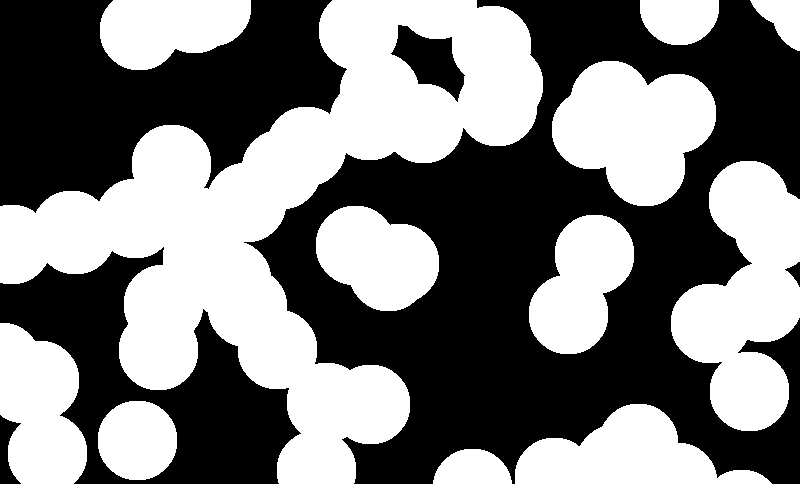
\includegraphics[width=0.9\linewidth]{images/disks-fragment.png}
  \caption[]{A fragment of overlapping disks used in testing of our library.}
  \label{fig:overlapping-disks}
\end{figure}

\subsection{Three-dimensional case}
Like in the previous case, consider an infinite set of balls with radii $R$ and
centers generated by Poisson point process with parameter $\lambda$. Closed-form
expressions for correlations functions are also known for this case.

Two-point function in this case is:
\begin{equation*}
  S_2(r) = e^{-\lambda\pi \left\{
  \begin{array}{ll}
    \frac{8}{3} R^3 & \quad r > 2R \\
    \frac{4}{3} R^3 + rR^2 - \frac{1}{12}r^3 & \quad \text{otherwise}
  \end{array}
  \right.}
\end{equation*}

Let $\eta = \frac{4}{3}\lambda \pi R^3$. Then an expression for $F_{ss}$ is
\begin{equation*}
  F_{ss}(r) = S_2(r) \left\{
  \begin{array}{ll}
    \frac{9\eta^2}{R^2} & \quad r > 2R \\
    \frac{9\eta^2}{R^2}(\frac{1}{2}+\frac{r}{4R})^2 + \frac{3\eta}{2rR} & \quad \text{otherwise}
  \end{array}
  \right.
\end{equation*}

Surface-void function $F_{sv}$ is:
\begin{equation*}
  F_{sv}(r) = \frac{3\eta}{R} S_2(r) \left\{
  \begin{array}{ll}
    1 & \quad r > 2R \\
    \frac{1}{2} + \frac{r}{4R} & \quad \text{otherwise}
  \end{array}
  \right.
\end{equation*}

Two-point function $L_2$:
\begin{equation*}
  L_2(r) = e^{-\lambda\pi (\frac{4}{3}R^3 + rR^2)}
\end{equation*}

Chord length function $p$:
\begin{equation*}
  p(r) = \pi\lambda R^2 e^{-\pi\lambda rR^2}
\end{equation*}

And finally pore size function $P$:
\begin{equation*}
  P(r) = 4\pi\lambda(r+R)^2 e^{-\frac{4}{3}\pi\lambda (r^3 + 3r^2R + 3rR^2)}
\end{equation*}

To test out package we generate a realization of random overlapping disks
(\cref{fig:overlapping-disks}) with dimensions $500 \times 500 \times 500$ and
parameters $R = 10\ px$ and $\lambda = 10^{-4}\ px^{-3}$ and compare calculated
correlation functions with their theoretical values. The results are present on
\cref{fig:verification}.

\begin{figure*}[tp]
  \centering
  \subfigure[Lineal-path correlation function]{
    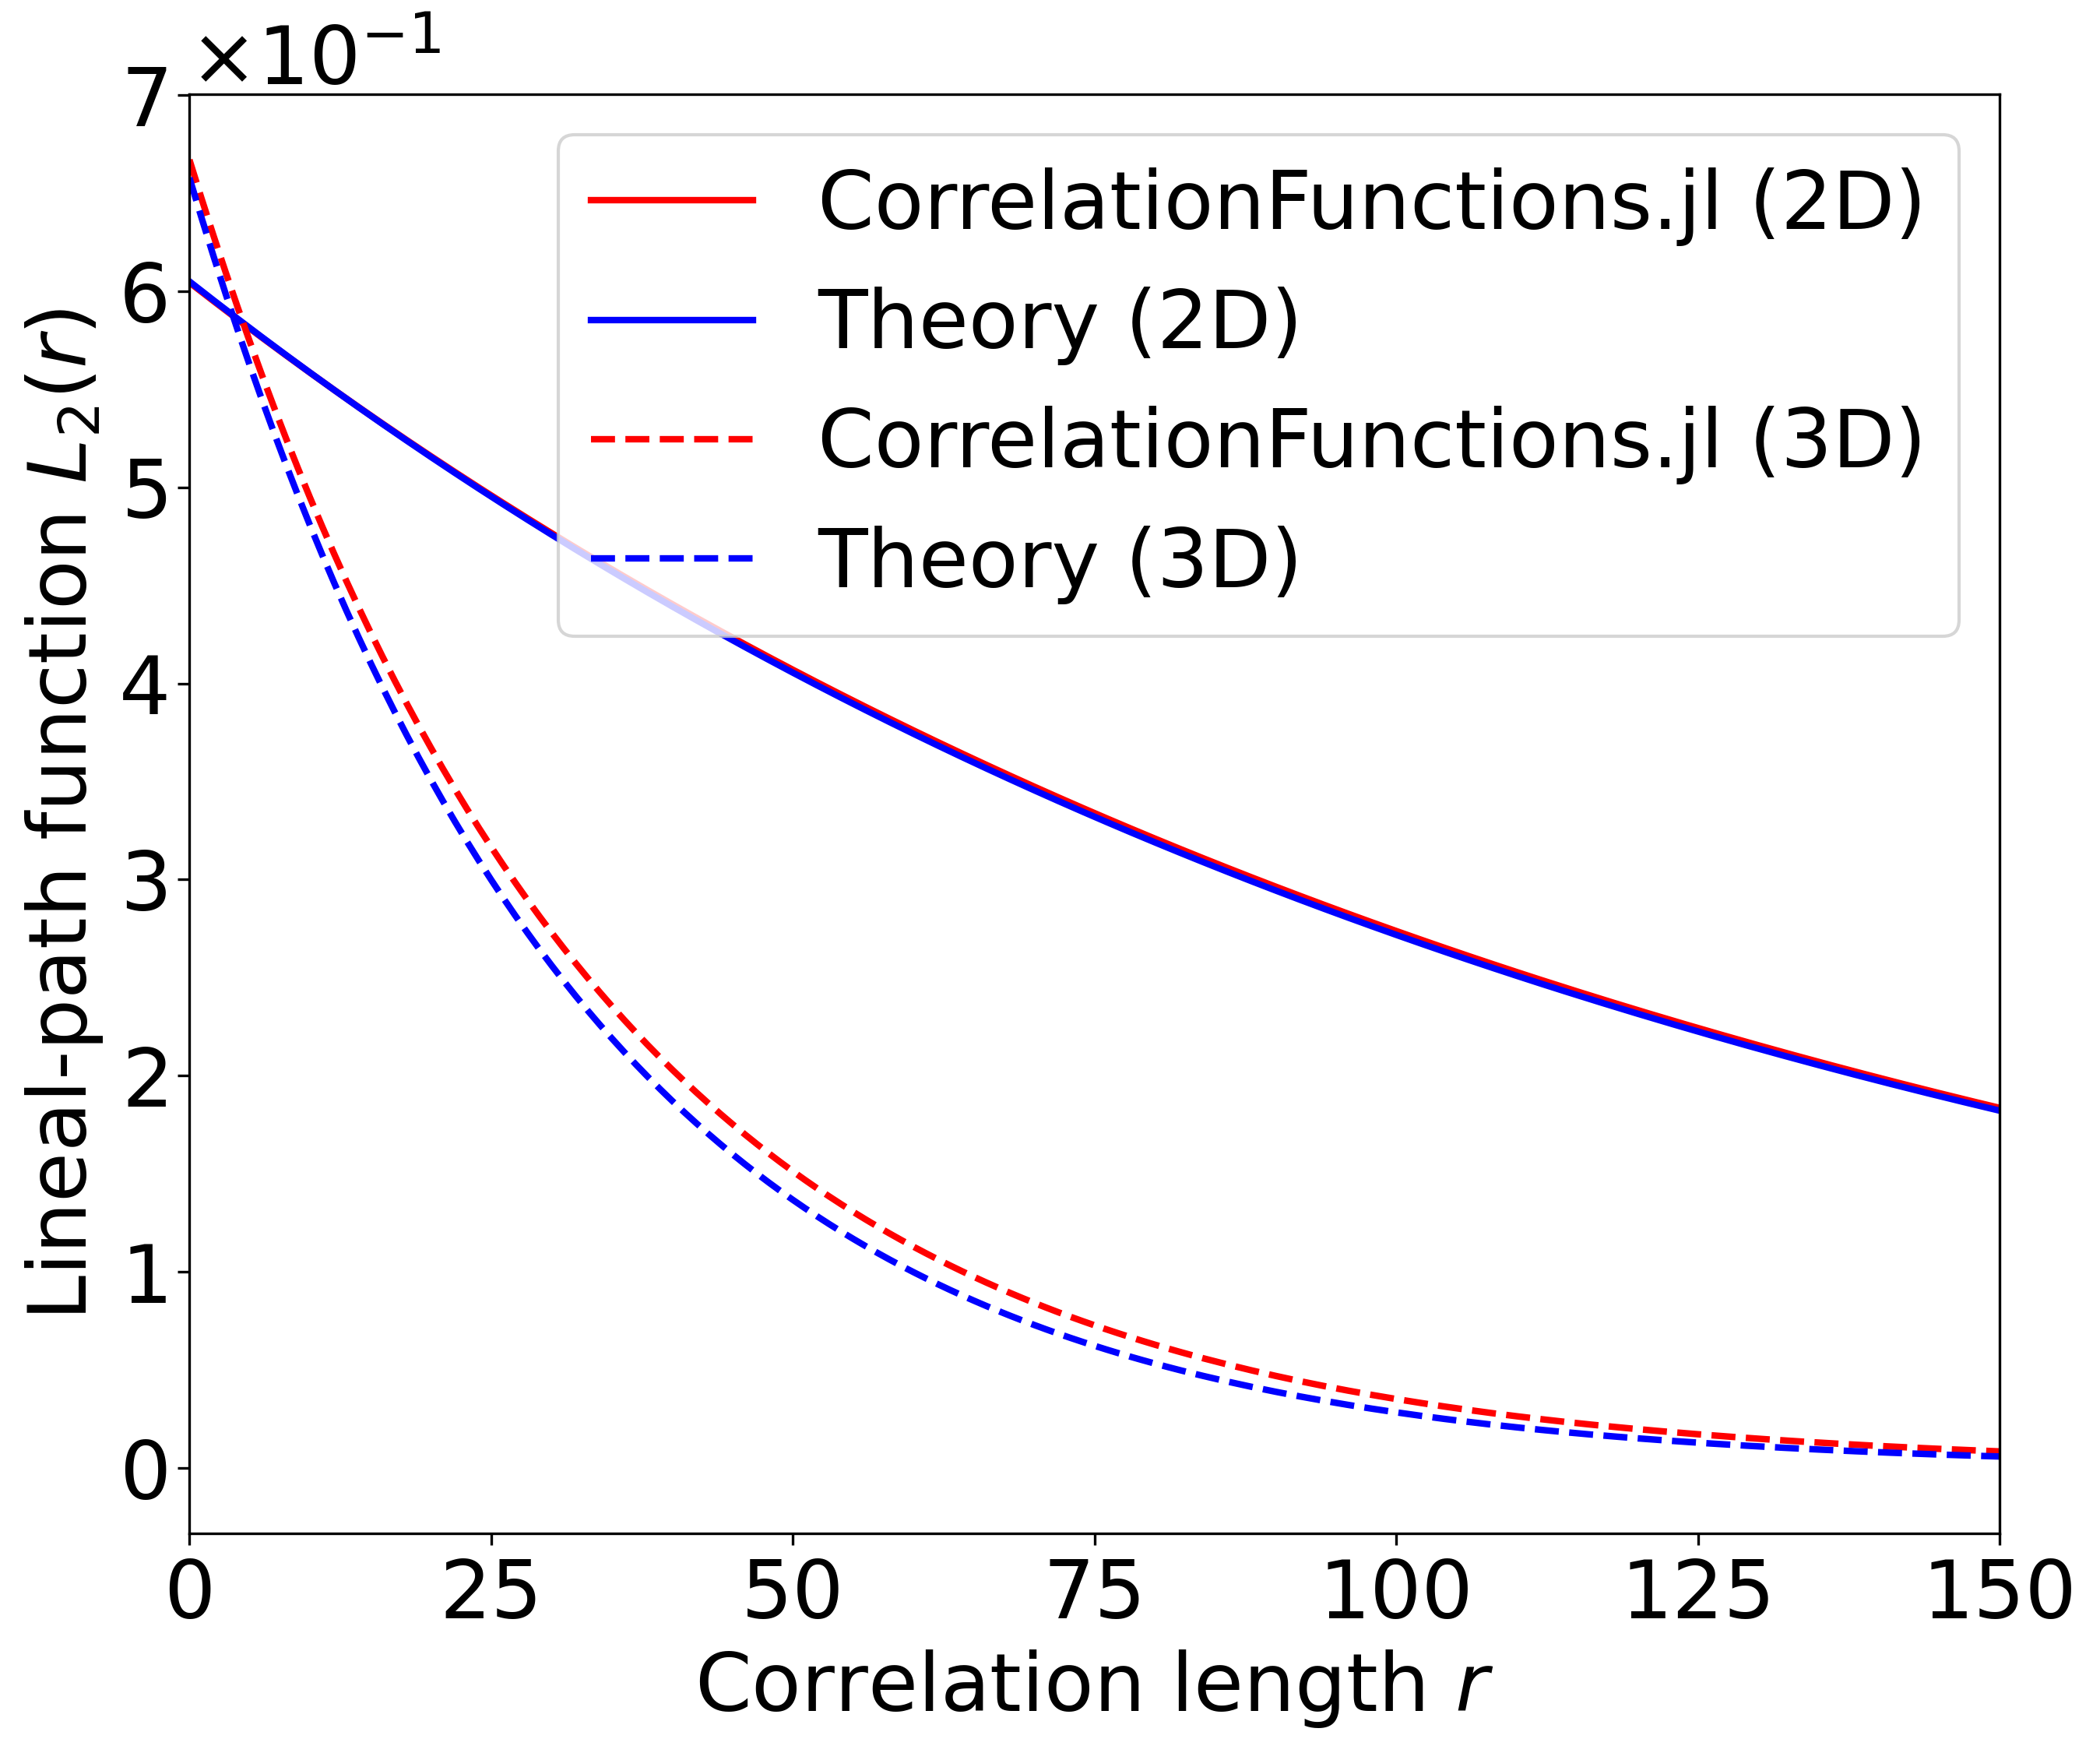
\includegraphics[width=0.3\linewidth]{images/l2.png}
    \label{fig:l2}}
  \hfill
  \subfigure[Two-point correlation function]{
    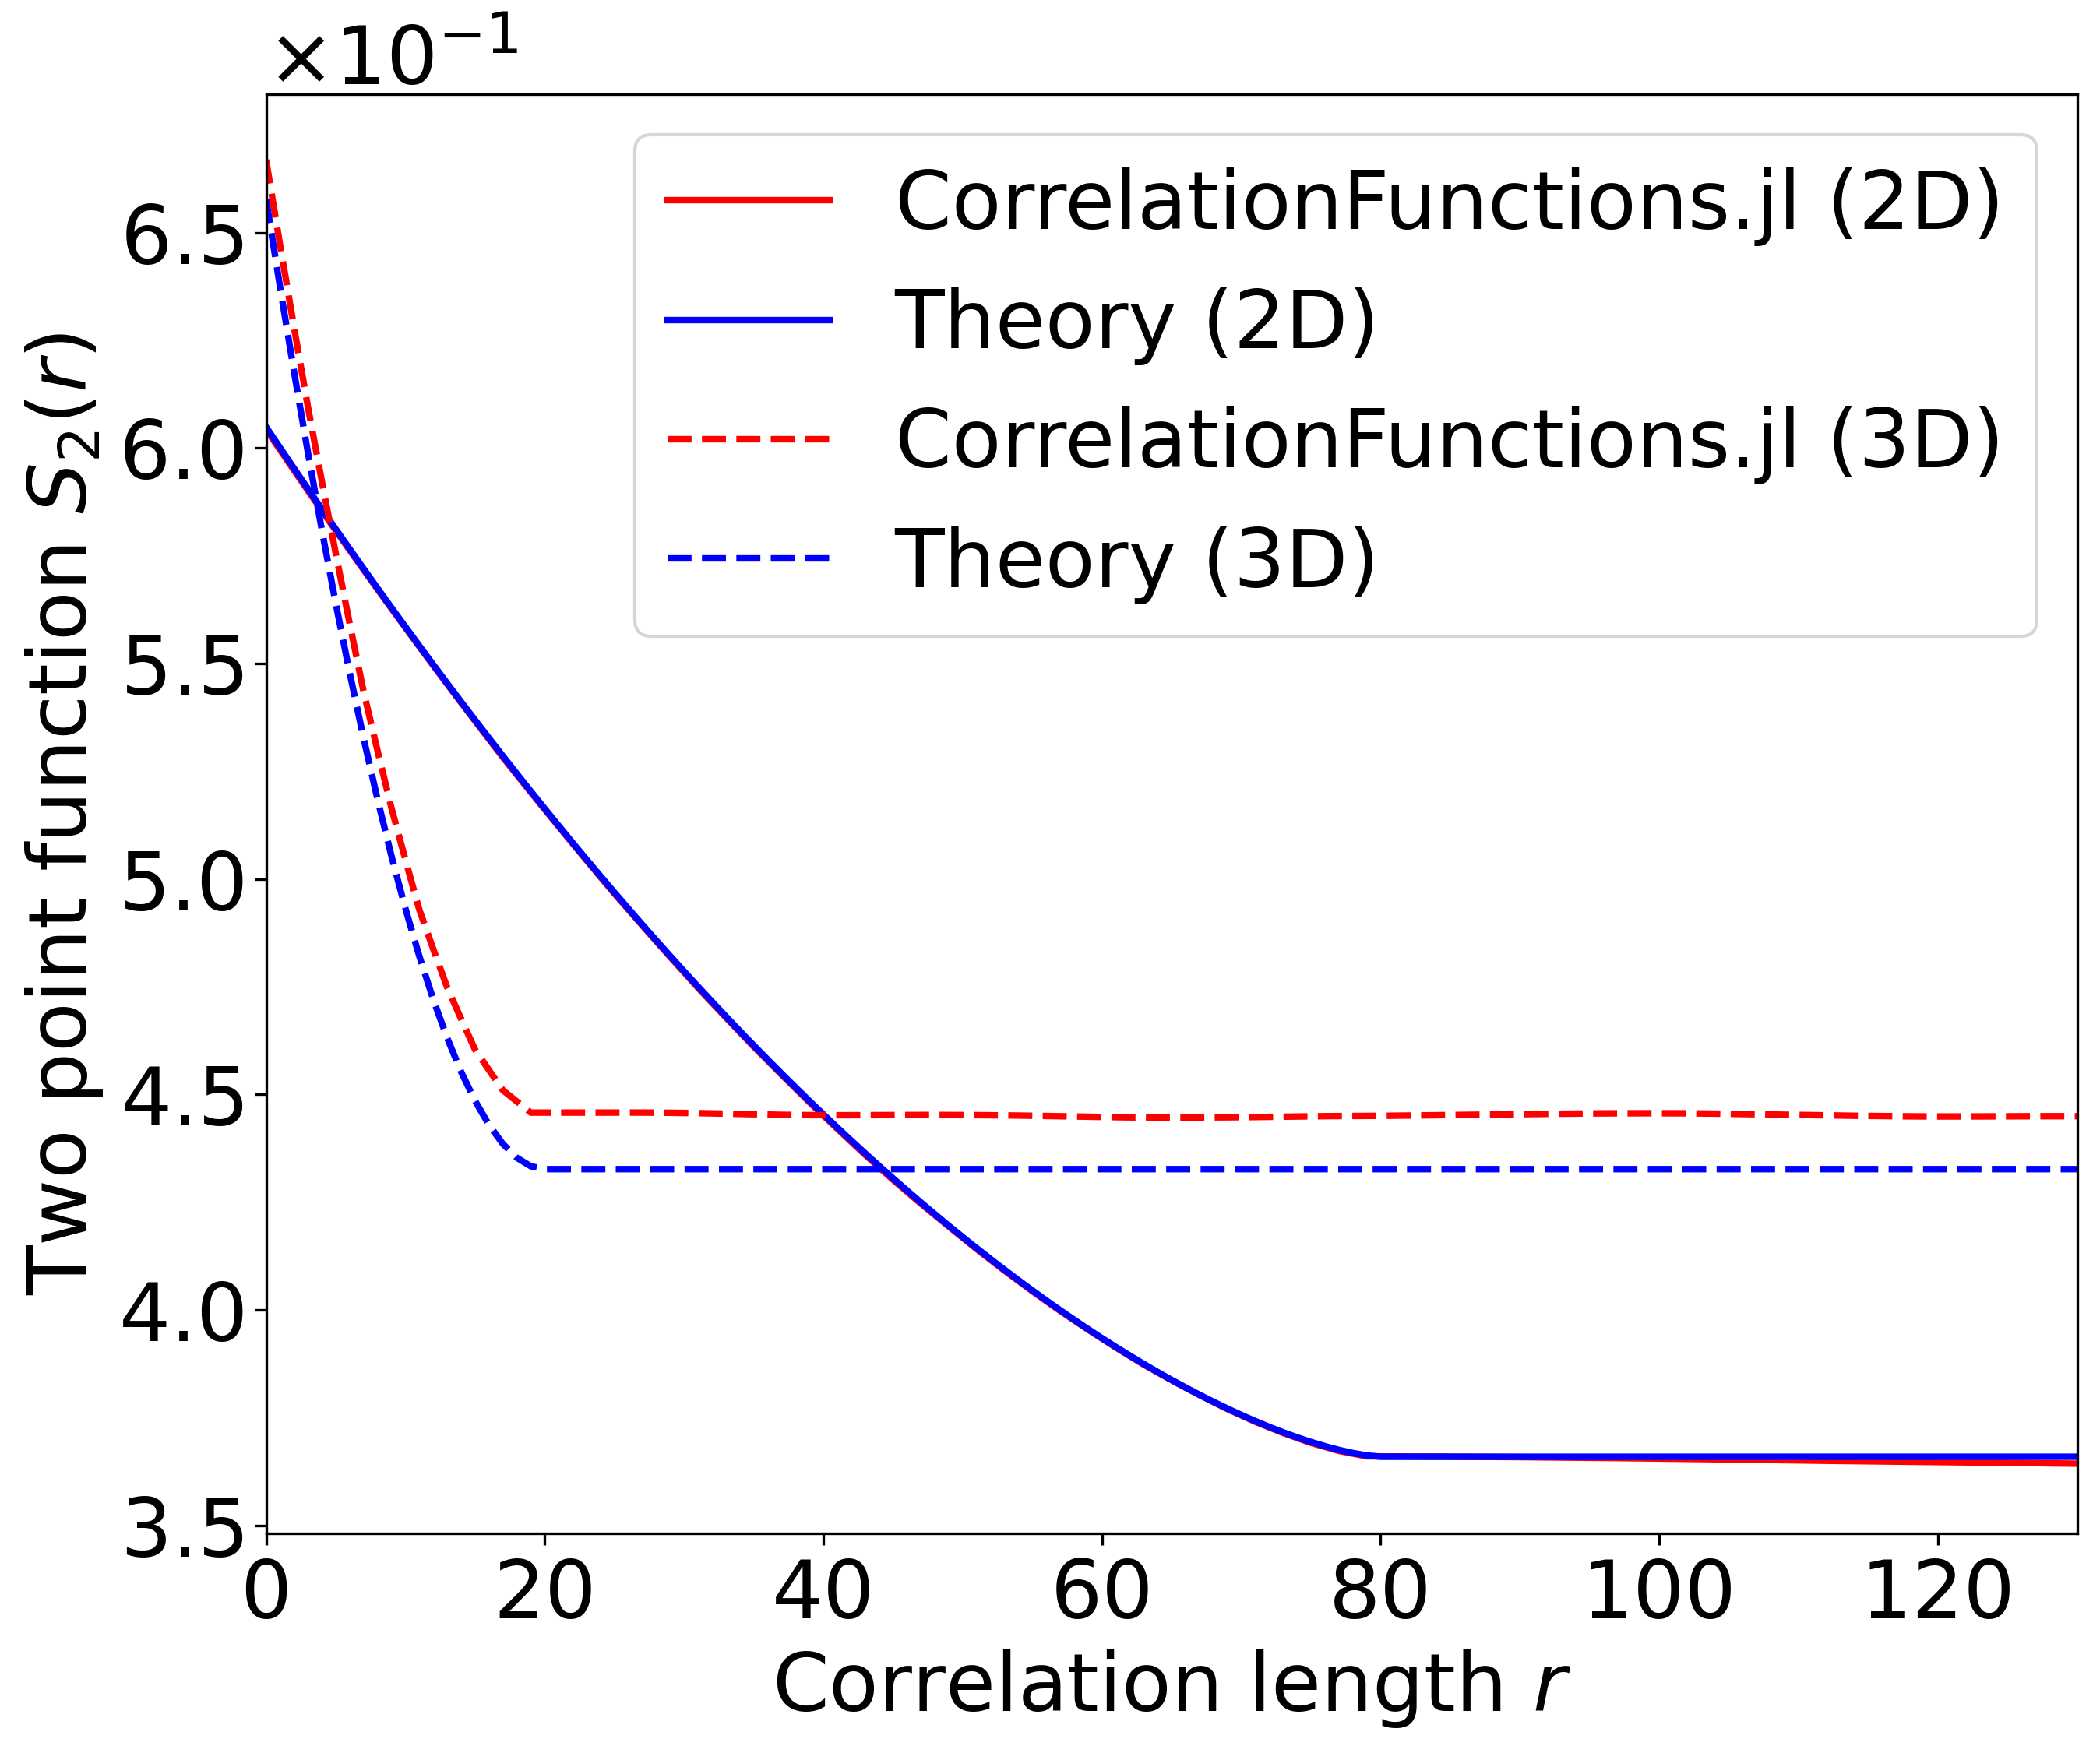
\includegraphics[width=0.3\linewidth]{images/s2.png}
    \label{fig:s2}}
  \hfill
  \subfigure[Surface-surface correlation function]{
    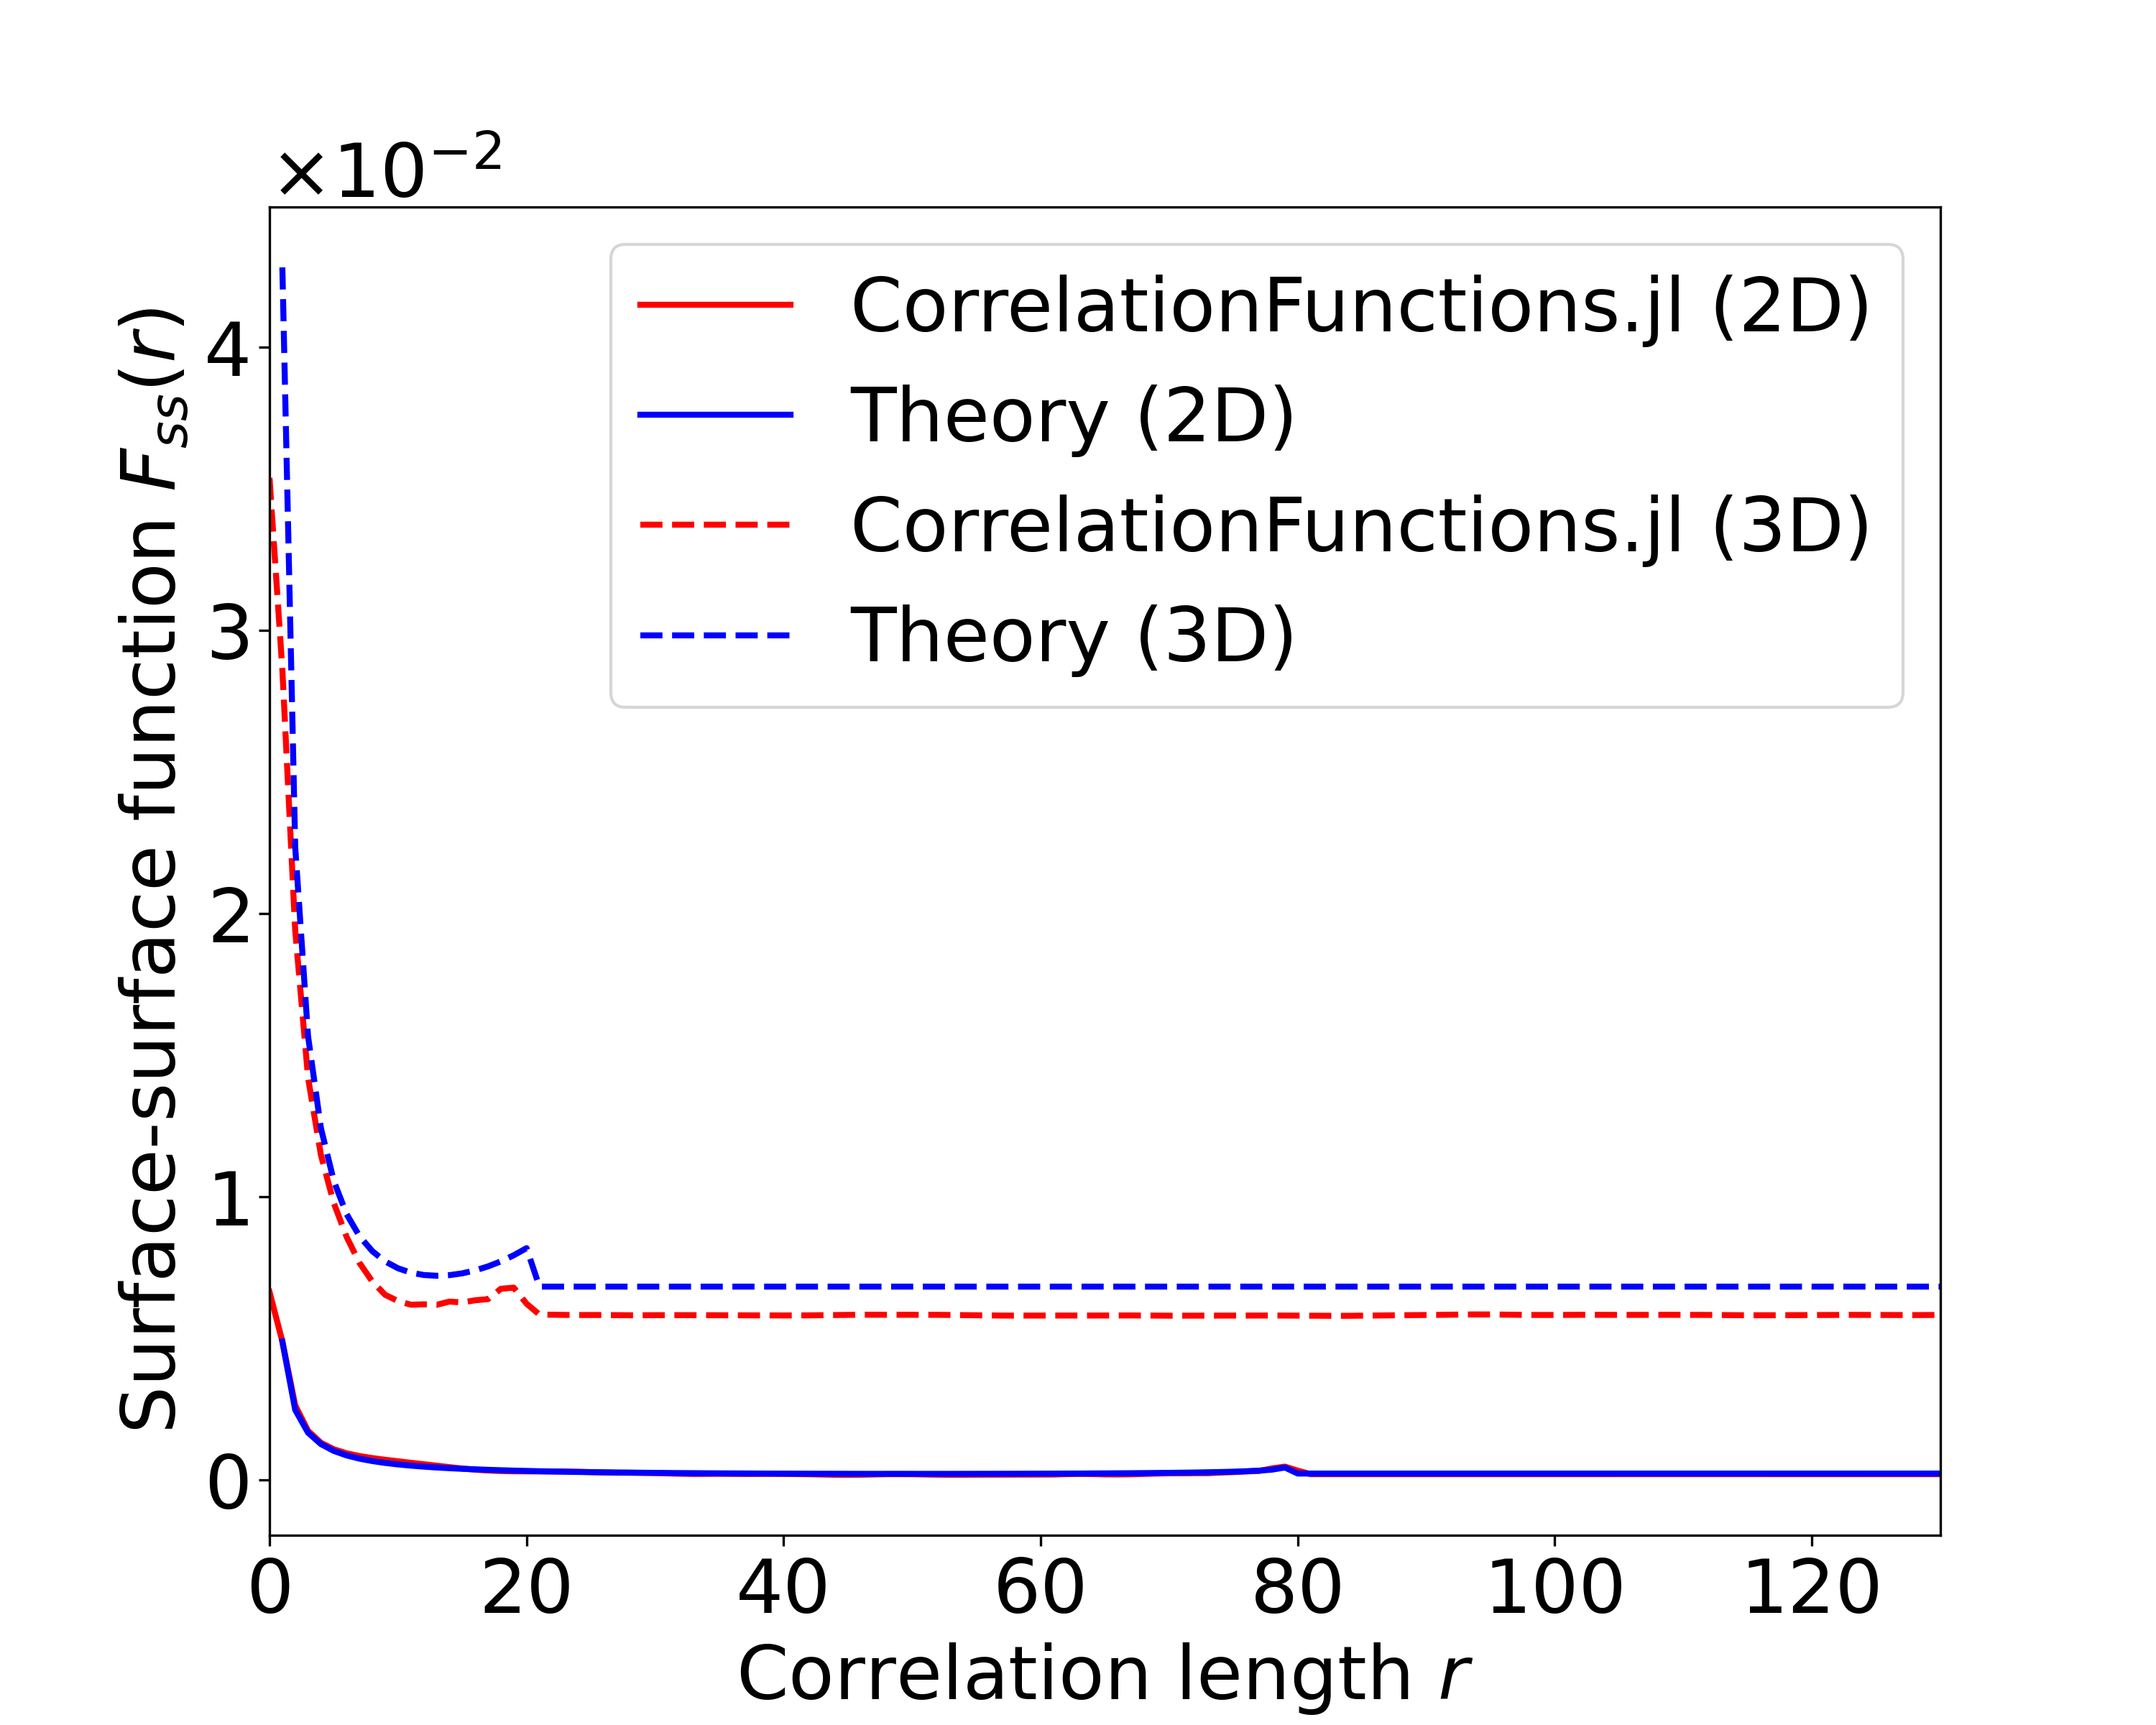
\includegraphics[width=0.3\linewidth]{images/ss.png}
    \label{fig:ss}}
  \vskip\baselineskip
  \subfigure[Surface-void correlation function]{
    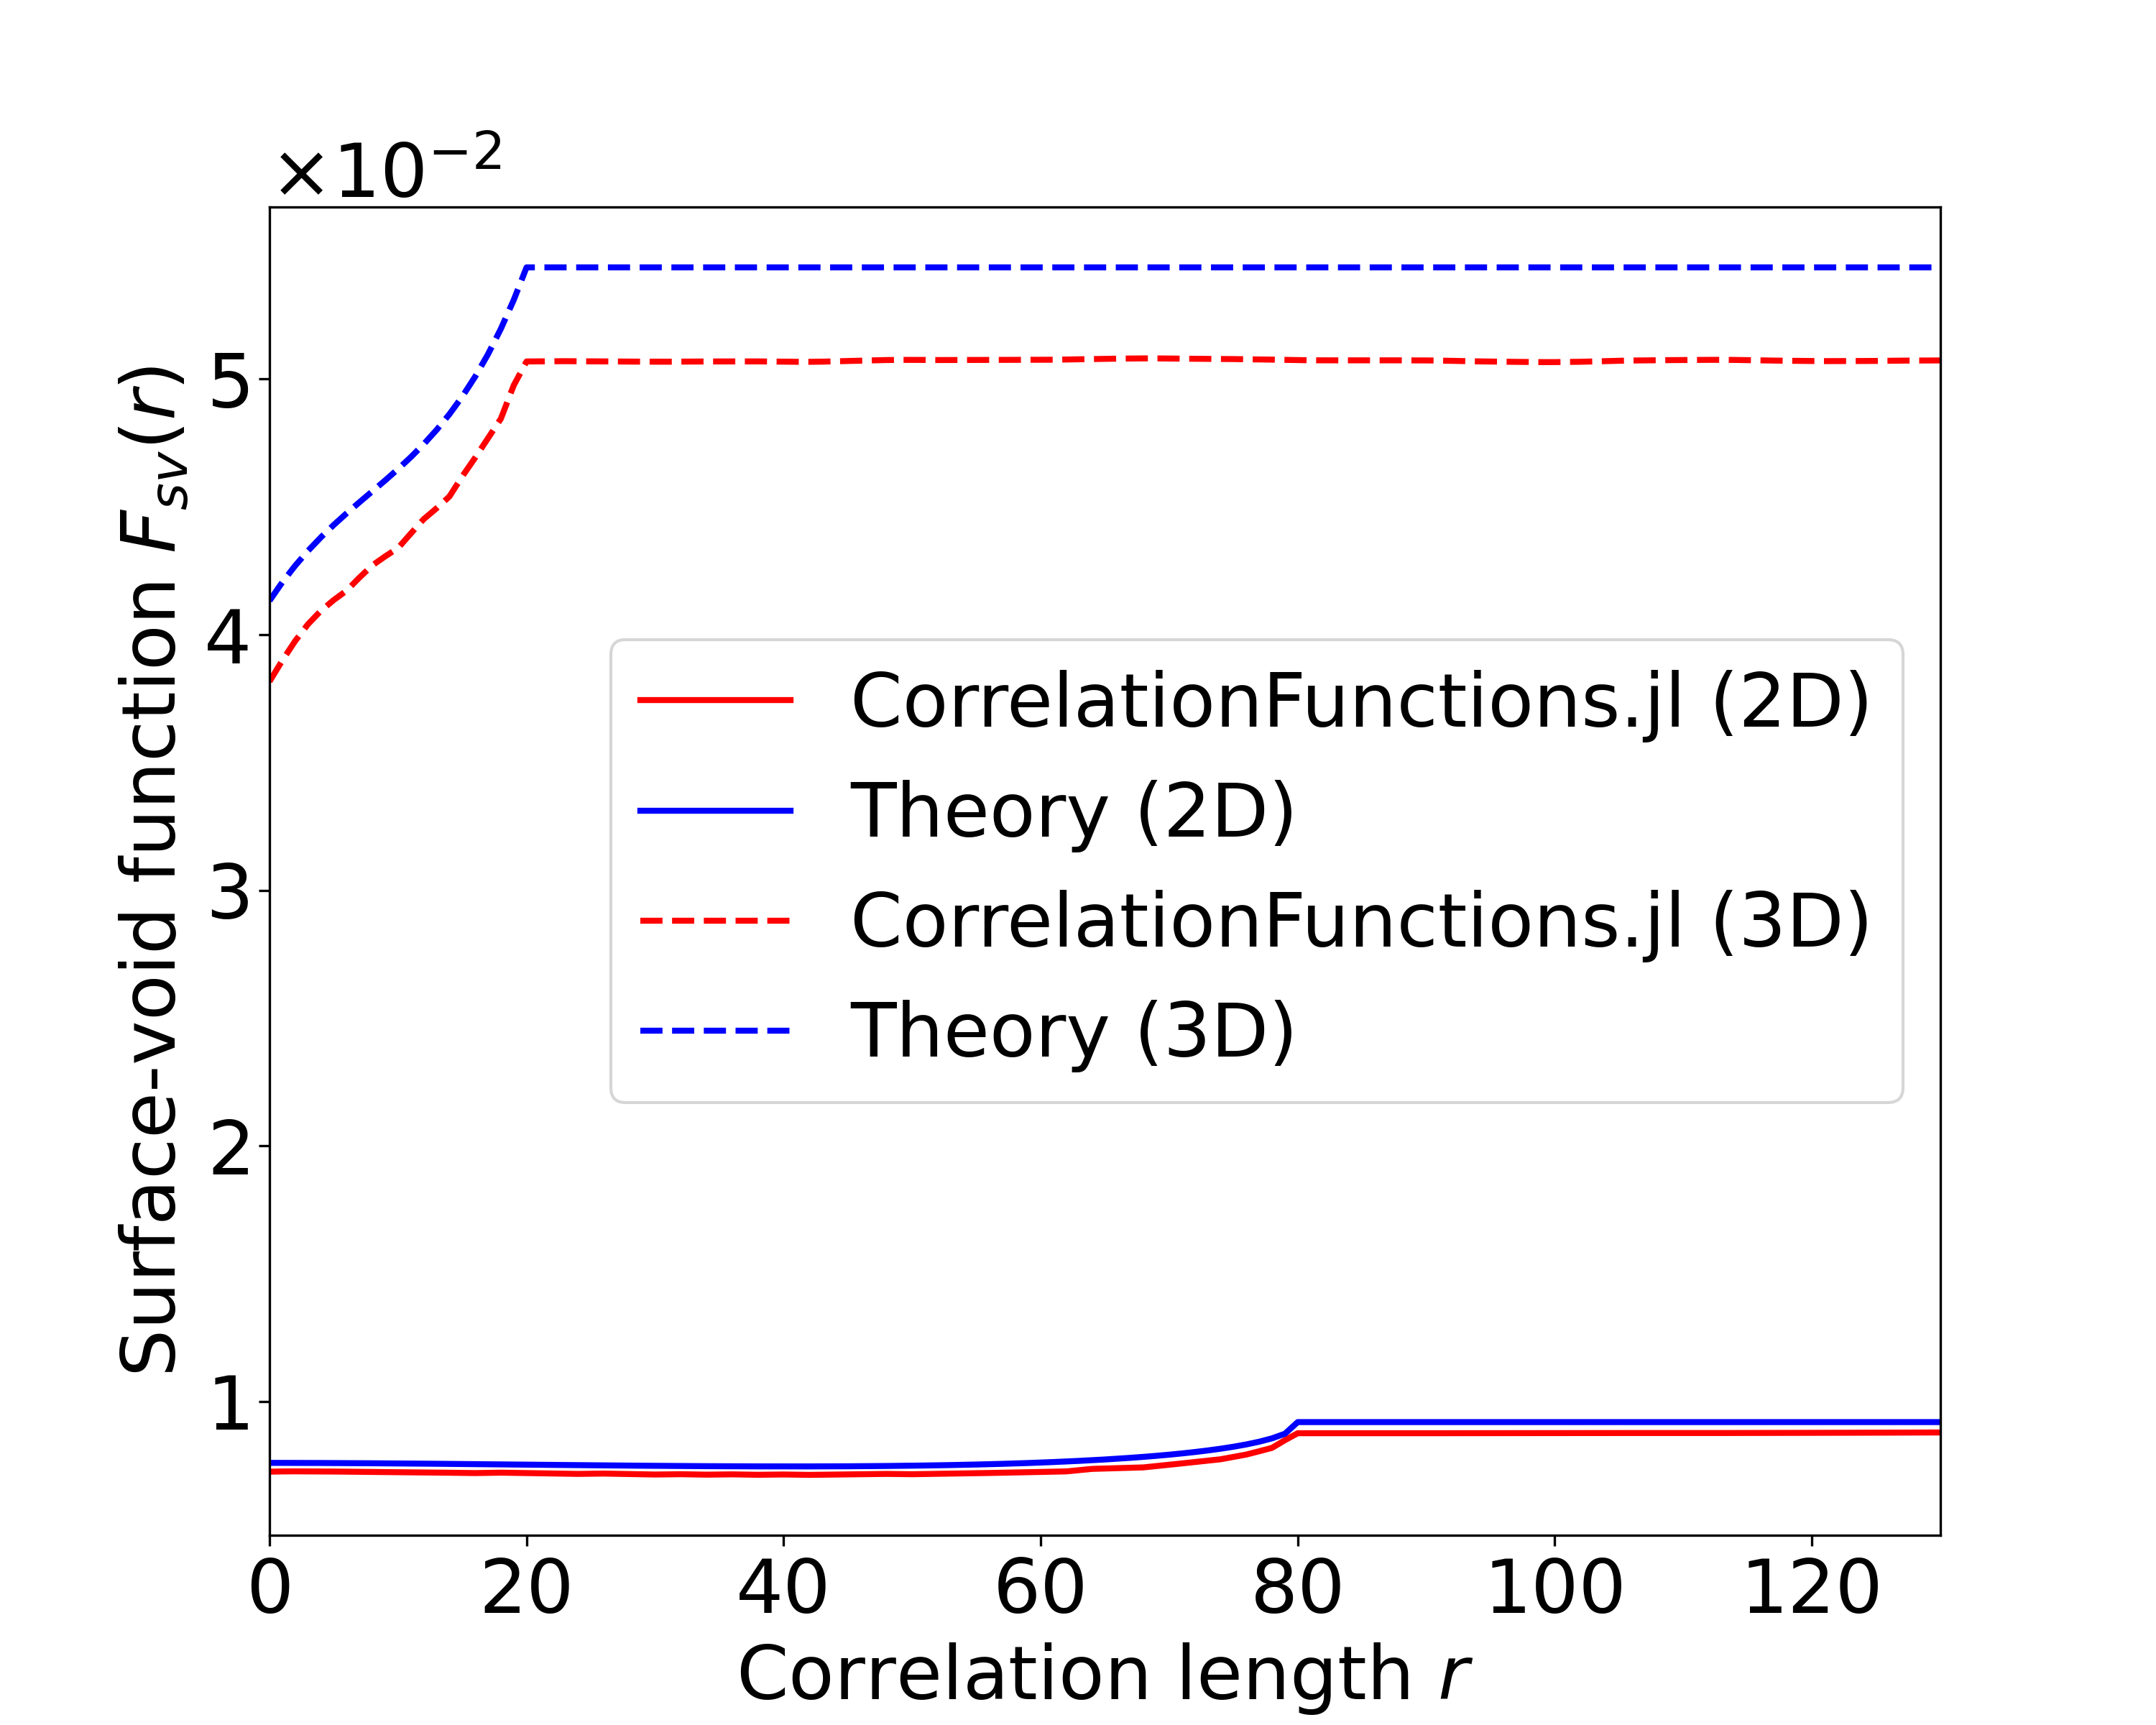
\includegraphics[width=0.3\linewidth]{images/sv.png}
    \label{fig:sv}}
  \hfill
  \subfigure[Pore size correlation function]{
    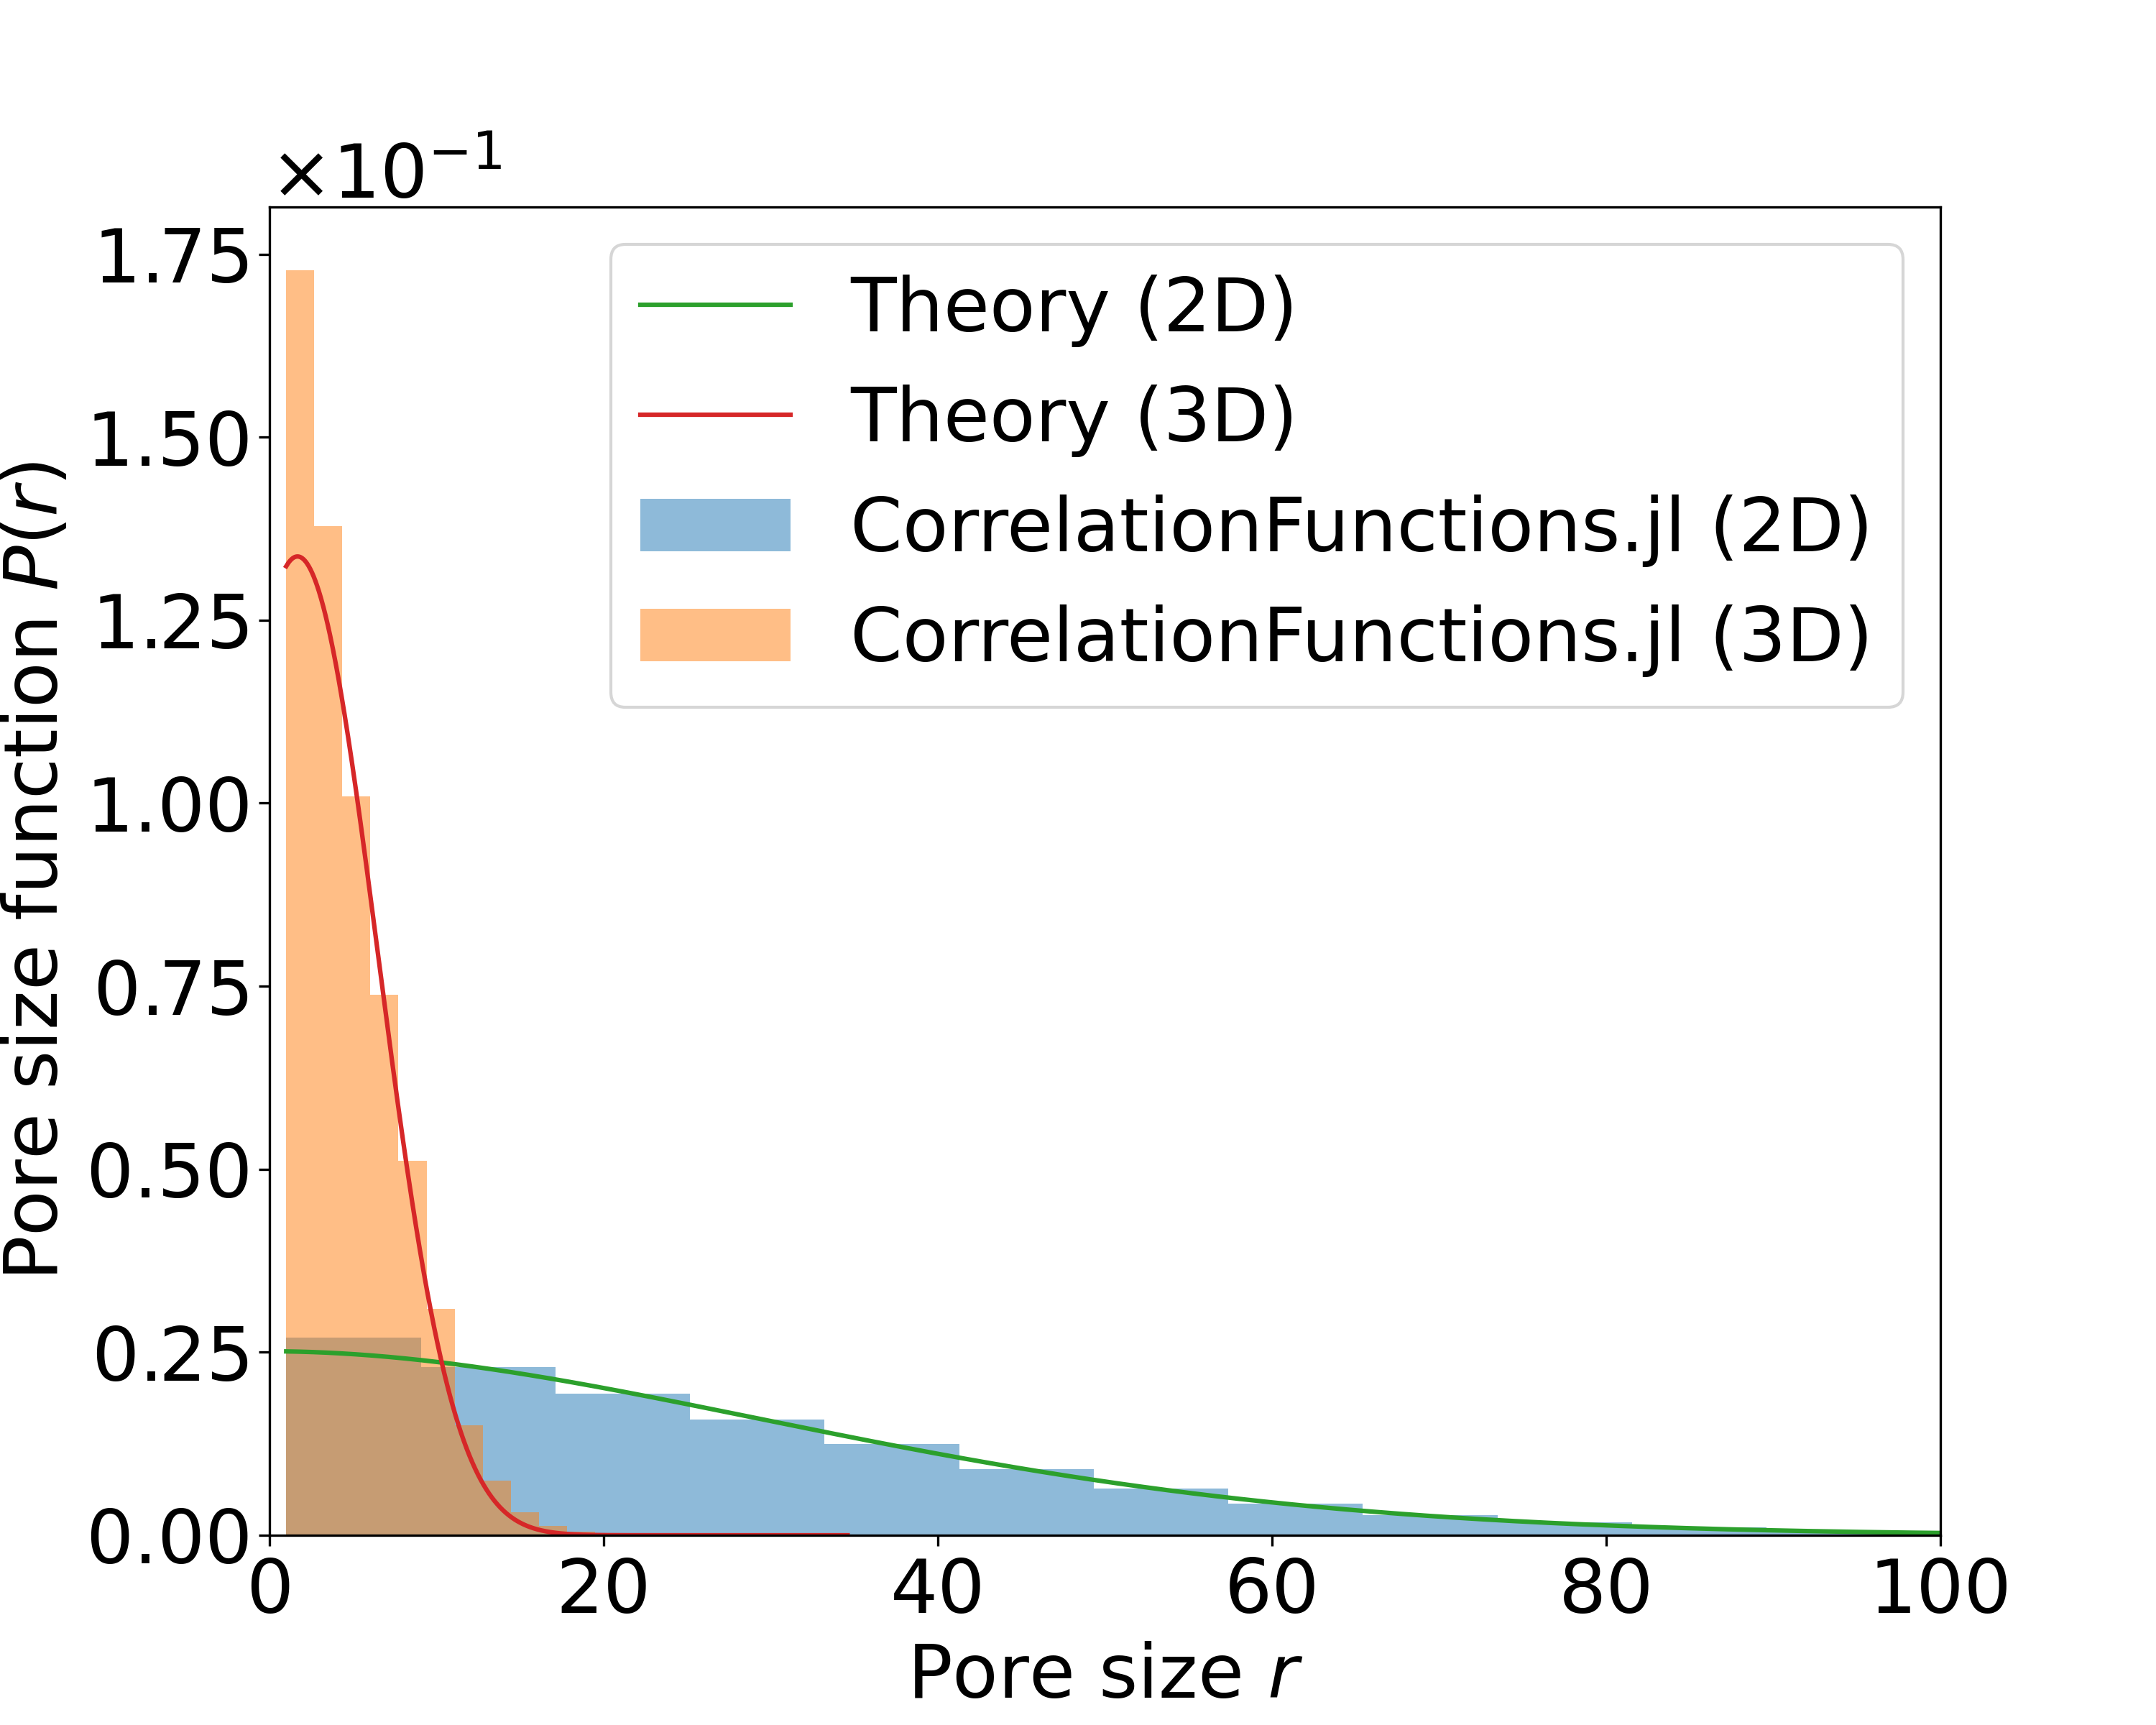
\includegraphics[width=0.3\linewidth]{images/ps.png}
    \label{fig:ps}}
  \hfill
  \subfigure[Chord length correlation function]{
    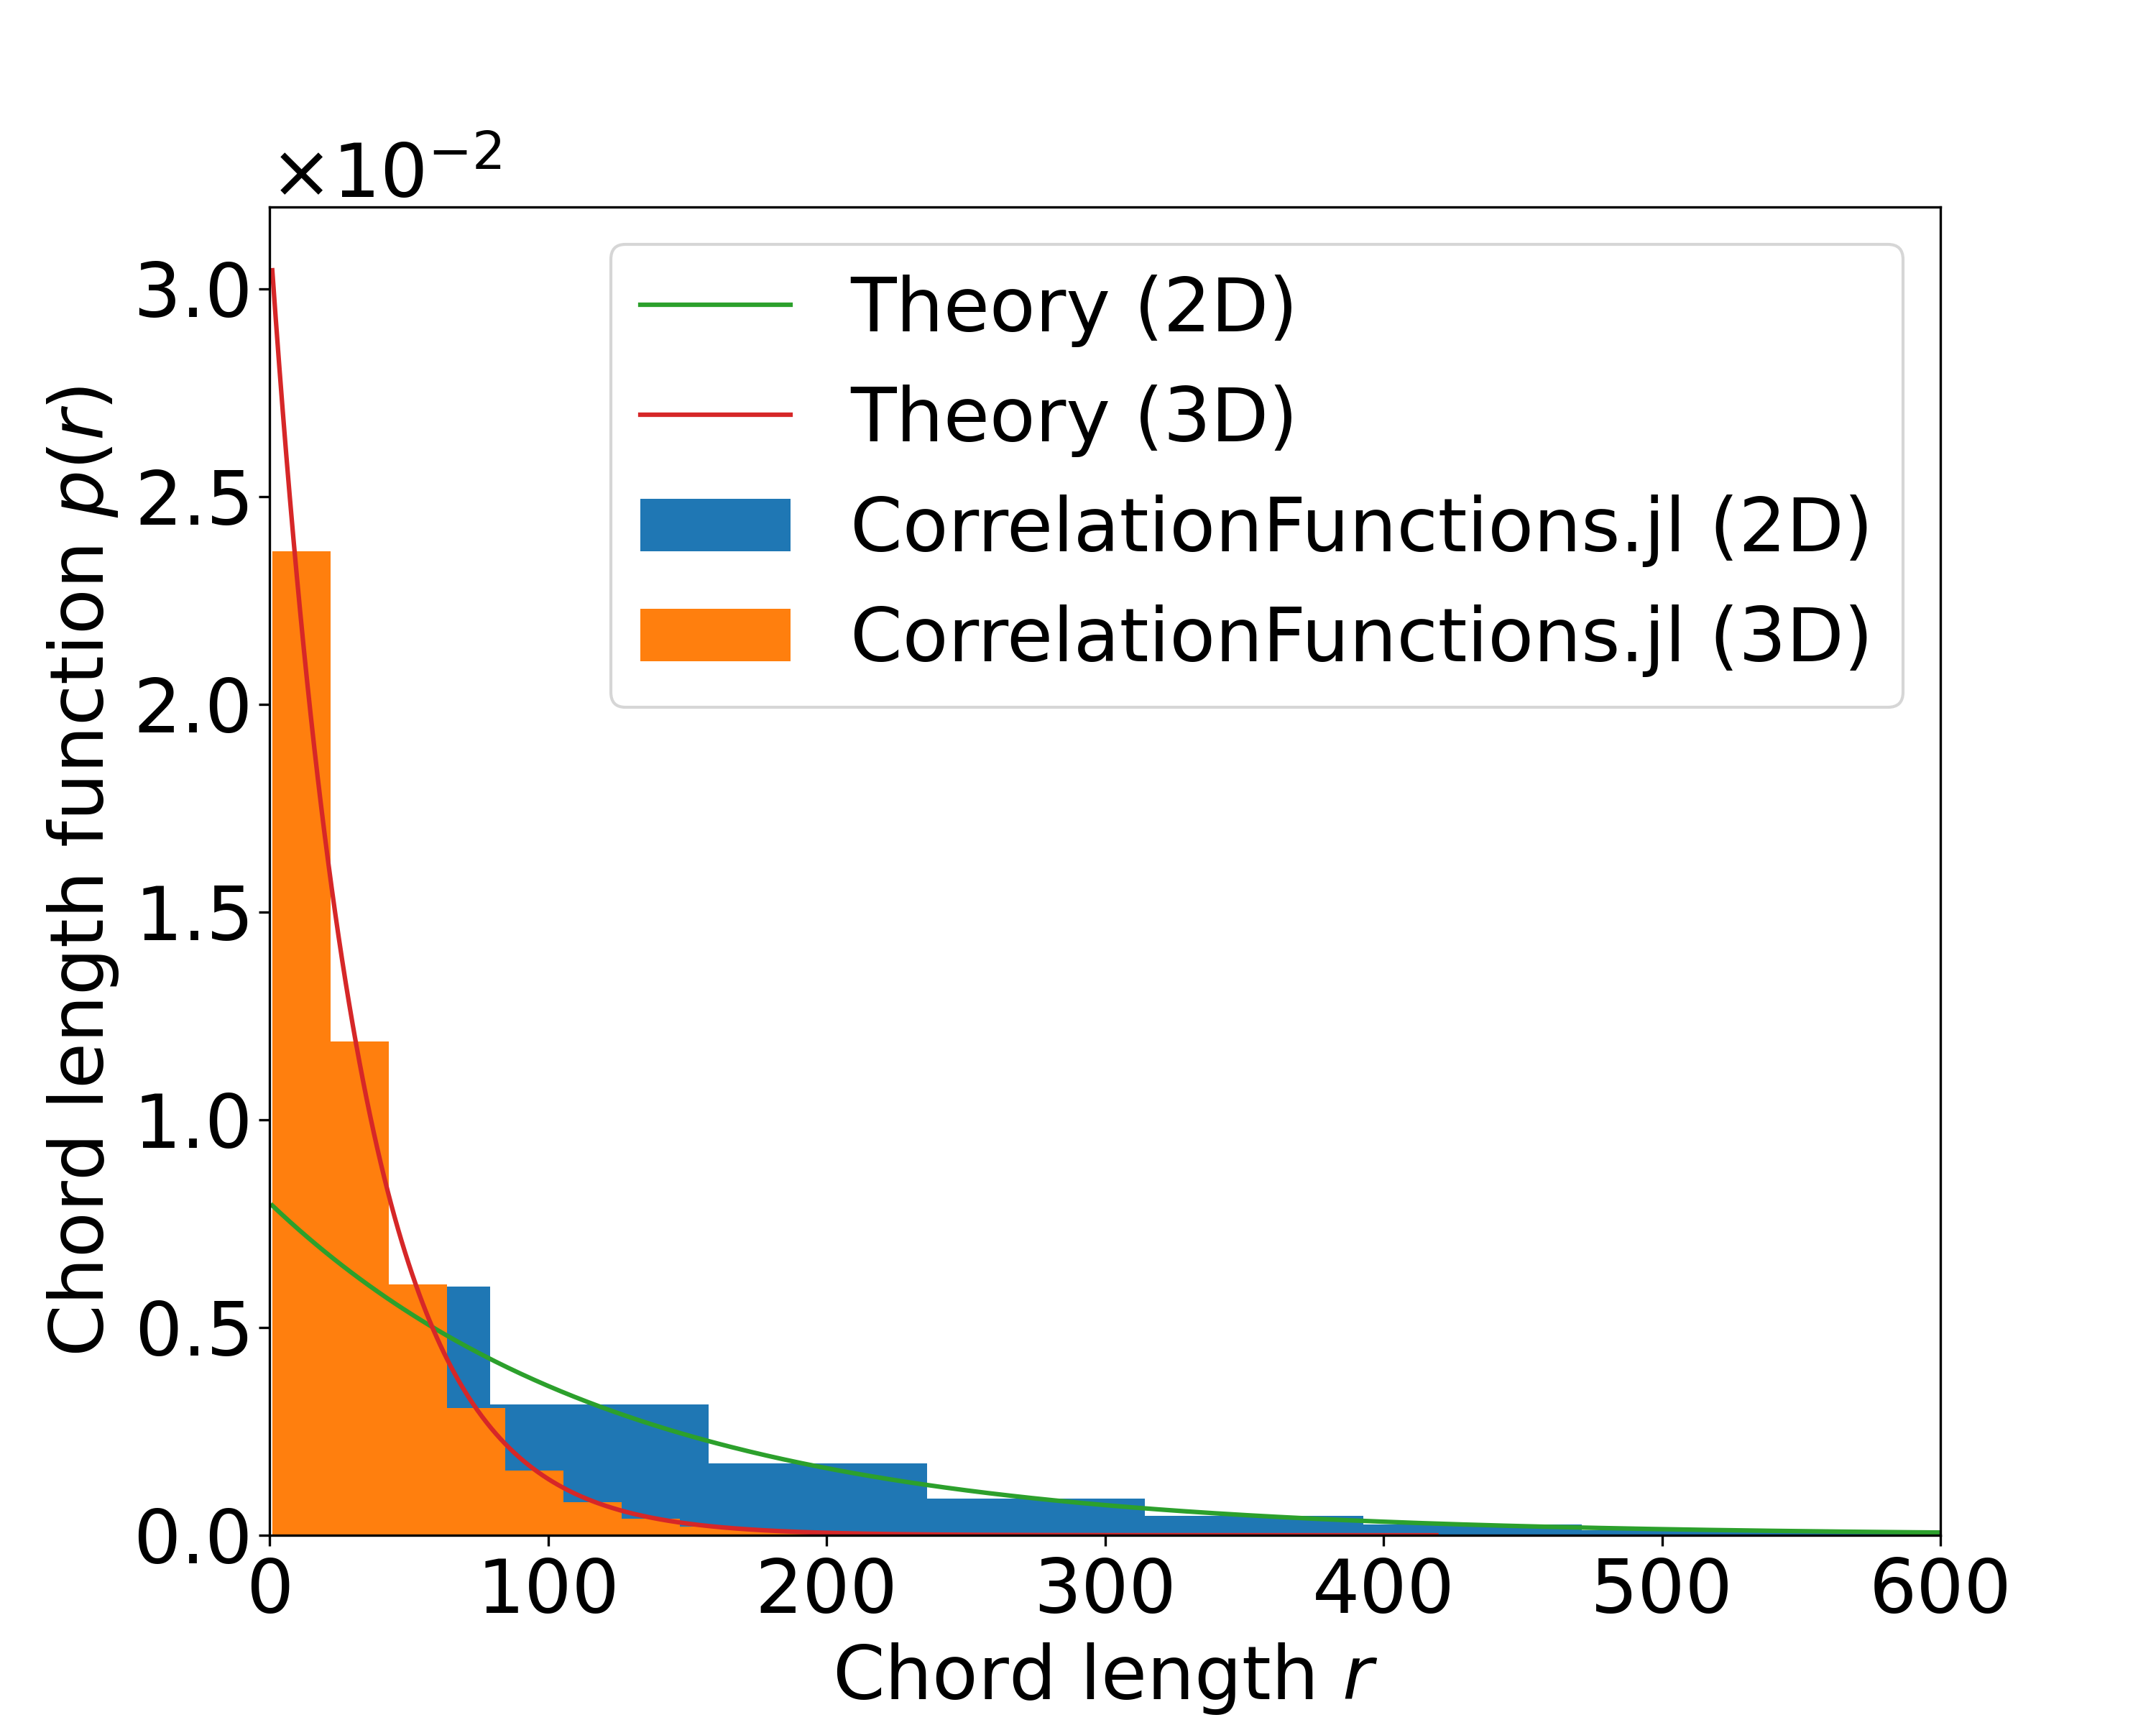
\includegraphics[width=0.3\linewidth]{images/cl.png}
    \label{fig:cl}}
  \caption[]{A comparison of calculated and theoretical values of correlation
    functions for overlapping disks and balls.}
  \label{fig:verification}
\end{figure*}

\section{Examples and applications}
\label{sec:examples}
After the verification of our computational approach based on analytical
solution we can apply our algorithms to evaluate correlation functions for
different porous media images, including real XCT and SEM images. A summary
which contains information about type of the images, dimensions and resolution
can be found in \cref{tab:samples}. XCT images of sandstones are provided by
Digital Rocks Portal\cite{DigitalRocks}. Correlation functions of these samples
can be seen on \cref{fig:real-data}.

\begin{table*}[!pt]
  \centering
  \begin{ruledtabular}
    \begin{tabular}{|c|c|c|c|}
      Sample name & Image type & Dimensions (pixels) & Image resolution ($\mu m$) \\
      \hline
      Bandera Brown sandstone & XCT & $1000 \times 1000 \times 1000$ & 2.25 \\
      Bentheimer sandstone    & XCT & $1000 \times 1000 \times 1000$ & 2.25 \\
      Kirby sandstone         & XCT & $1000 \times 1000 \times 1000$ & 2.25 \\
      Sandstone 1 & SEM &  $1280 \times 869$ & 0.10 \\
      Sandstone 2 & SEM &  $1280 \times 869$ & 0.05 \\
      Carbonate 1 & SEM &  $1024 \times 691$ & 0.06
    \end{tabular}
  \end{ruledtabular}
  \caption{Summary of samples used for calculation of correlation functions.}
  \label{tab:samples}
\end{table*}

\begin{figure*}[pt]
  \centering
  \subfigure[Bandera Brown sandstone]{
    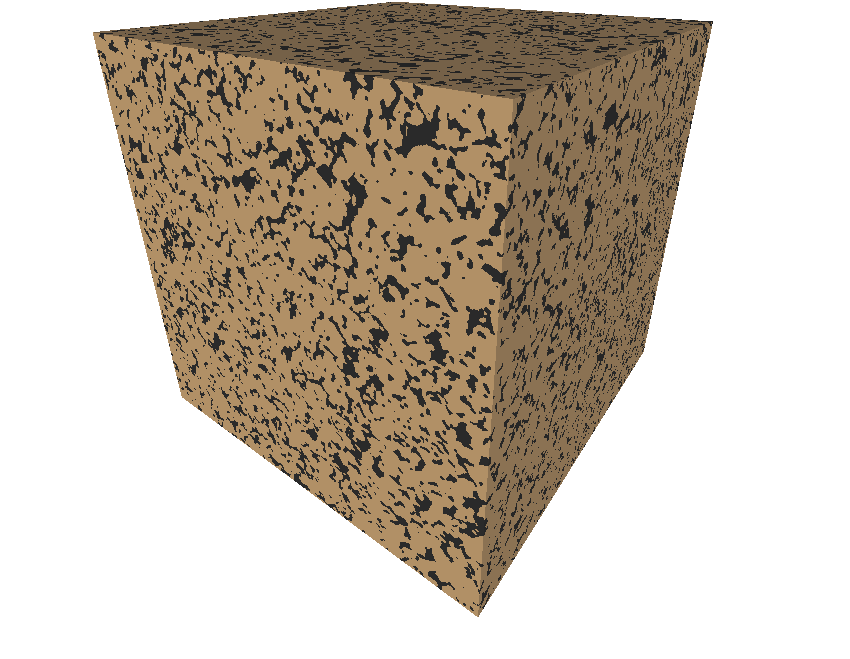
\includegraphics[width=0.3\linewidth]{real-data/BanderaBrown_2d25um_binary.png}
    \label{fig:bandera}}
  \hfill
  \subfigure[Bentheimer sandstone]{
    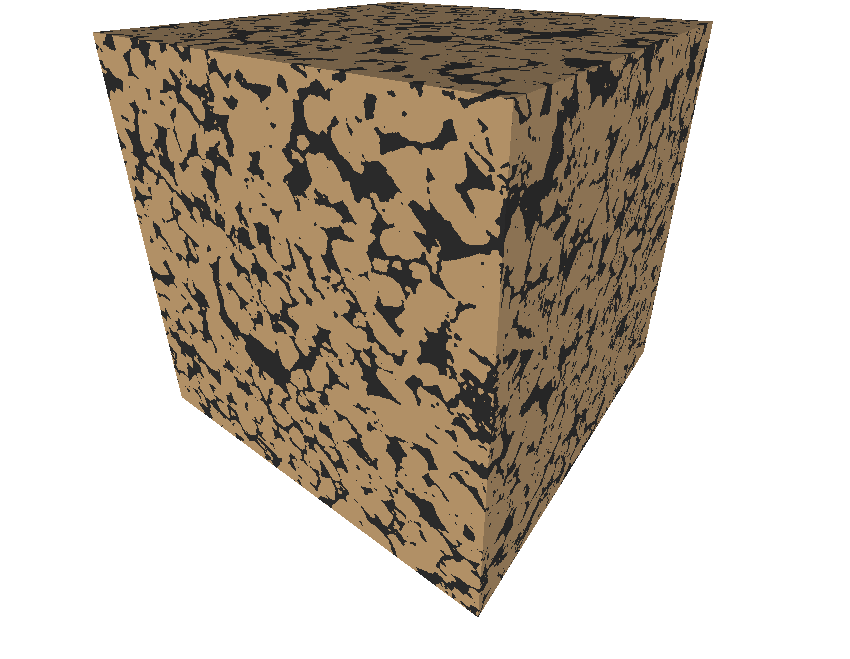
\includegraphics[width=0.3\linewidth]{real-data/Bentheimer_2d25um_binary.png}
    \label{fig:bentheimer}}
  \hfill
  \subfigure[Kirby sandstone]{
    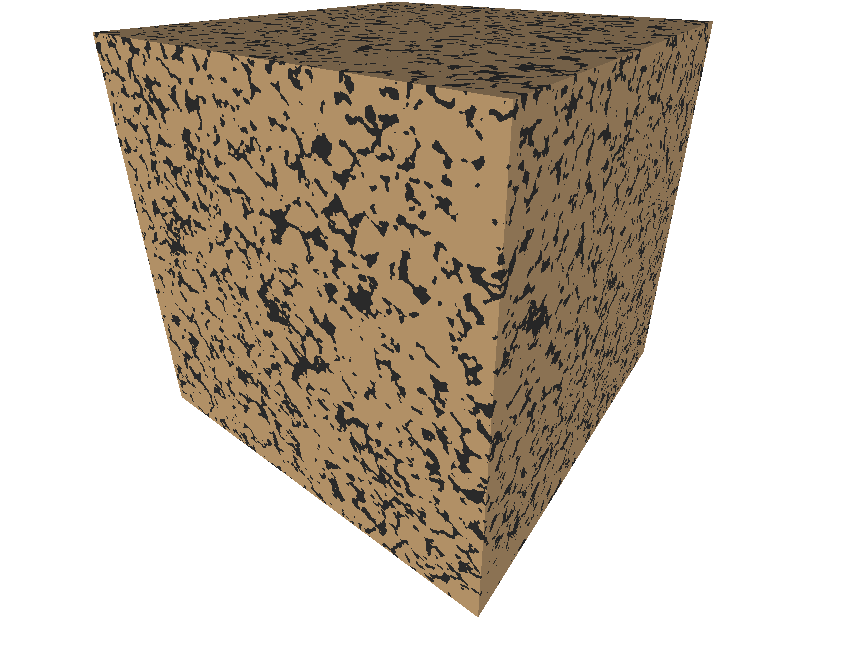
\includegraphics[width=0.3\linewidth]{real-data/Kirby_2d25um_binary.png}
    \label{fig:kirby}}
  \vskip\baselineskip
  \subfigure[Bandera Brown sandstone (correlation functions)]{
    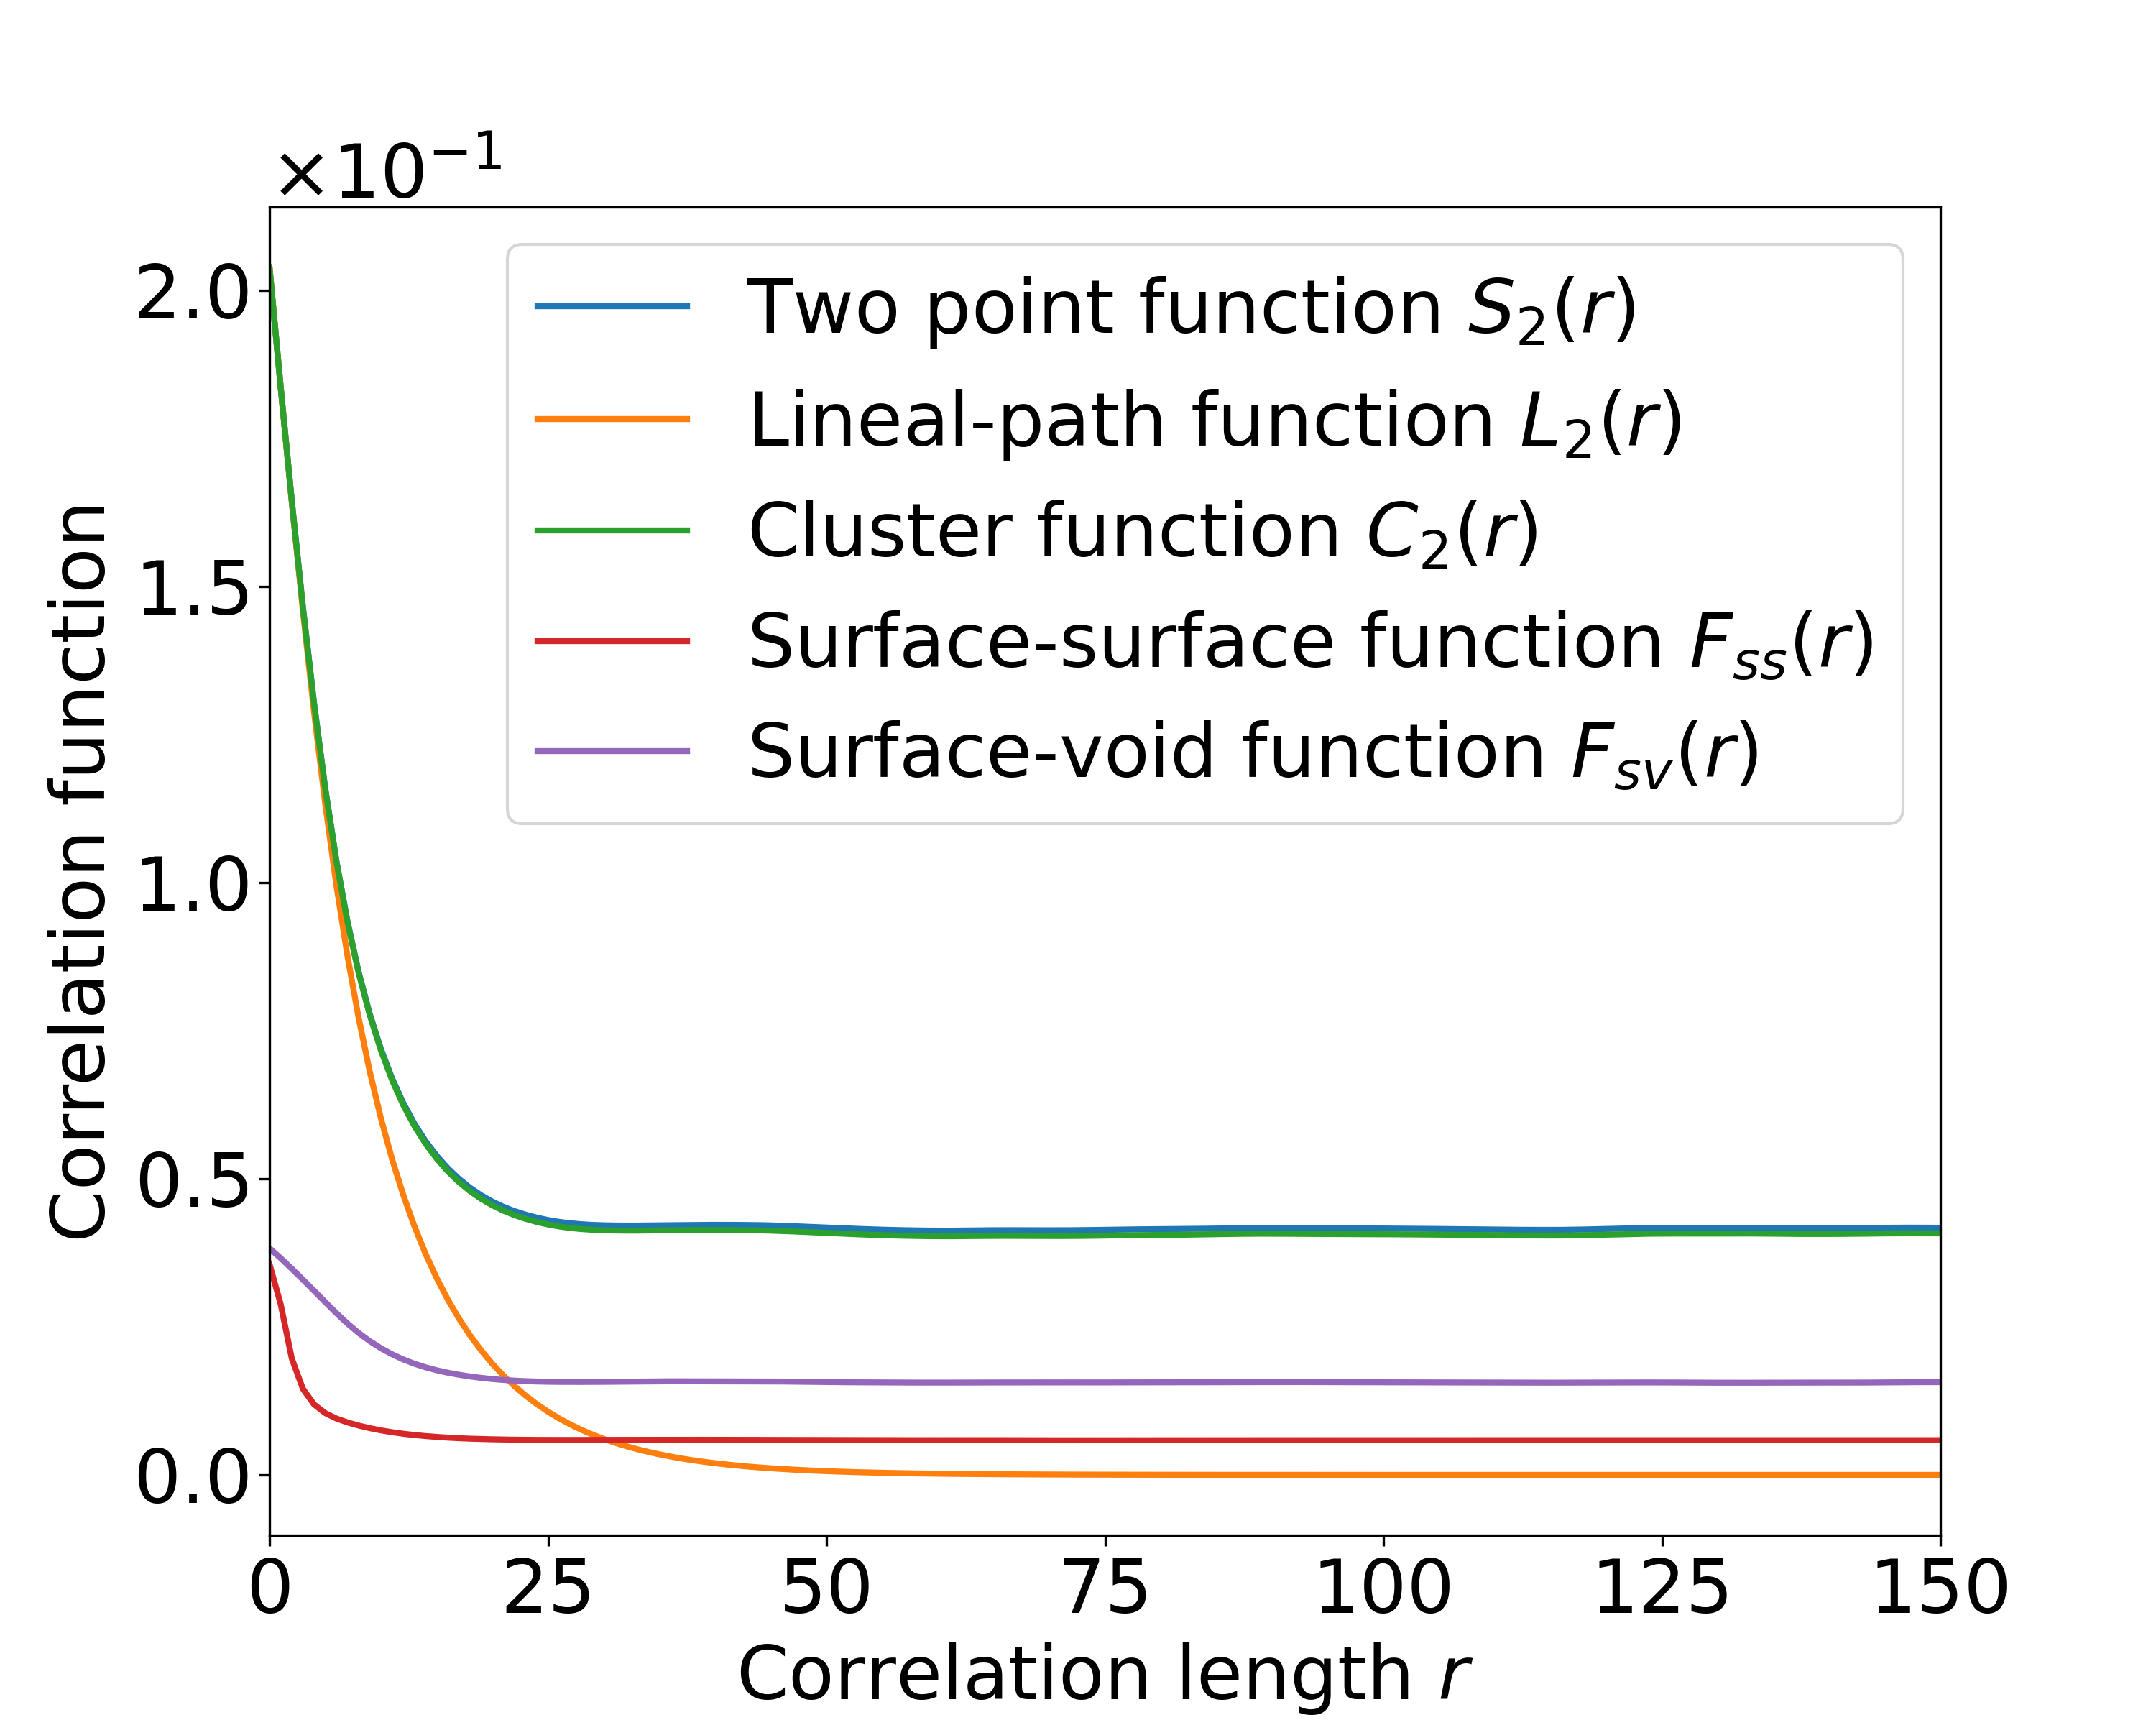
\includegraphics[width=0.3\linewidth]{real-data/BanderaBrown_2d25um_binary-plot.png}
    \label{fig:bandera-plt}}
  \hfill
  \subfigure[Bentheimer sandstone (correlation functions)]{
    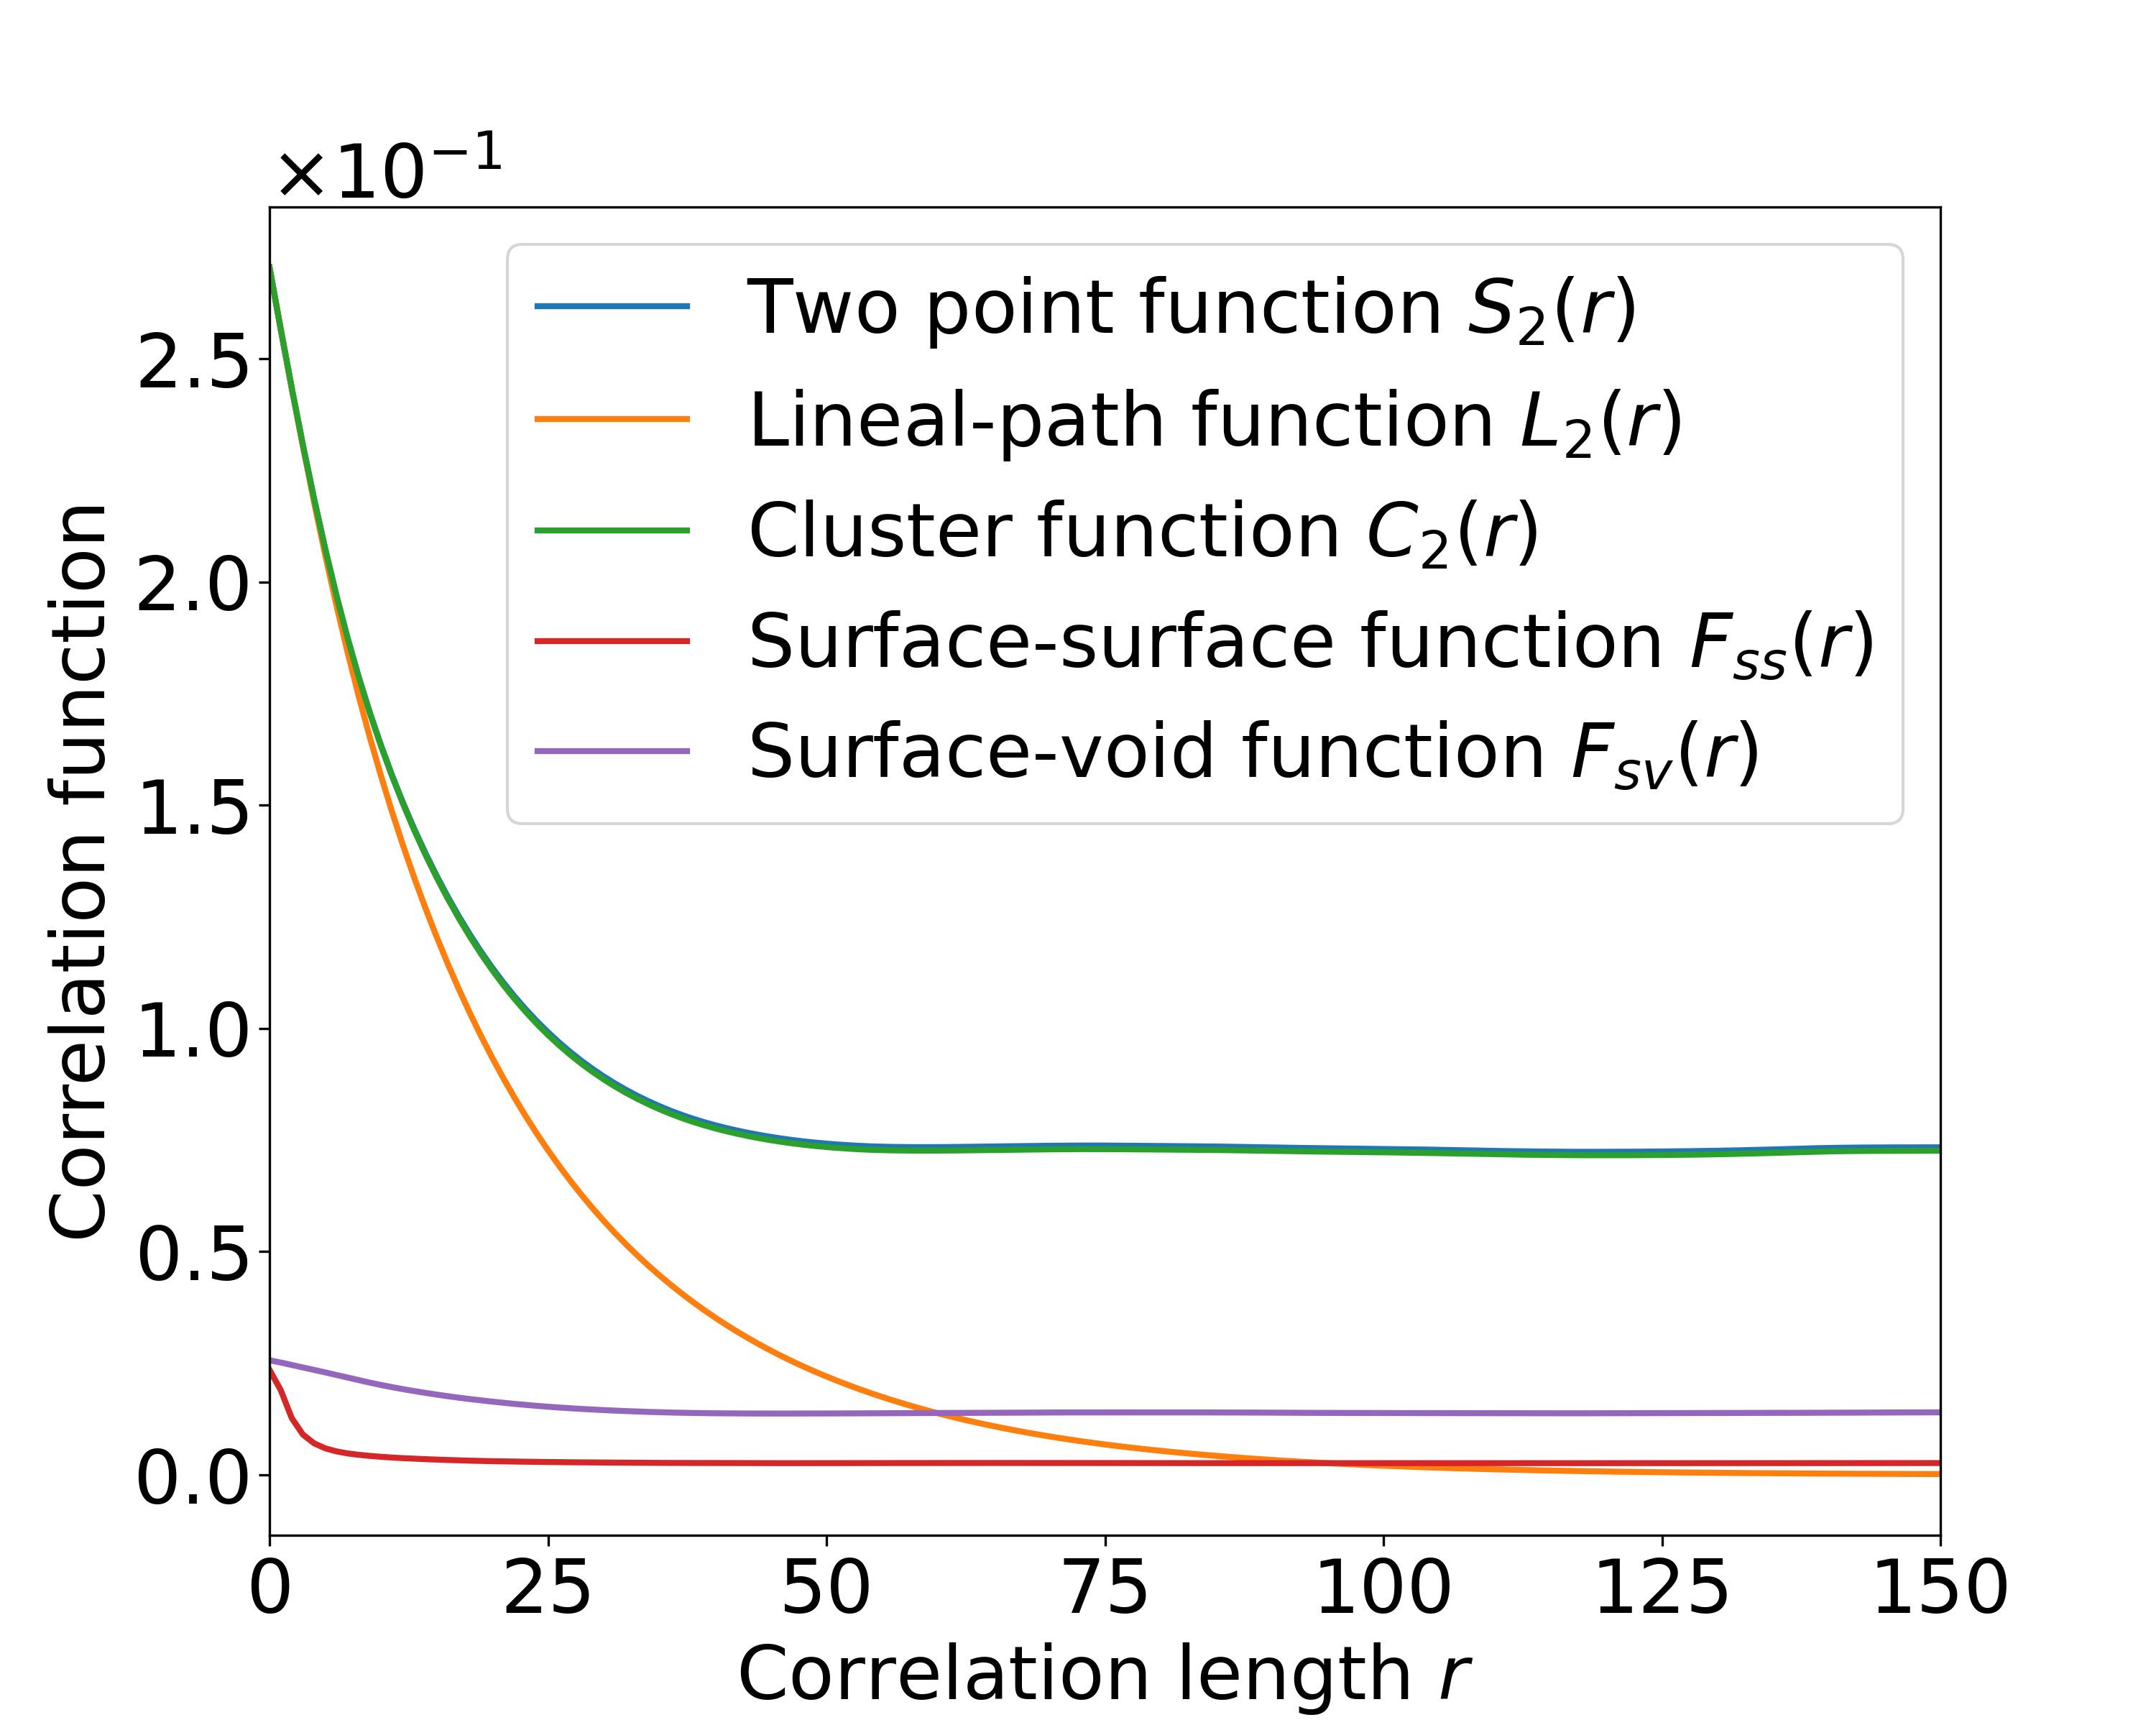
\includegraphics[width=0.3\linewidth]{real-data/Bentheimer_2d25um_binary-plot.png}
    \label{fig:bentheimer-plt}}
  \hfill
  \subfigure[Kirby sandstone (correlation functions)]{
    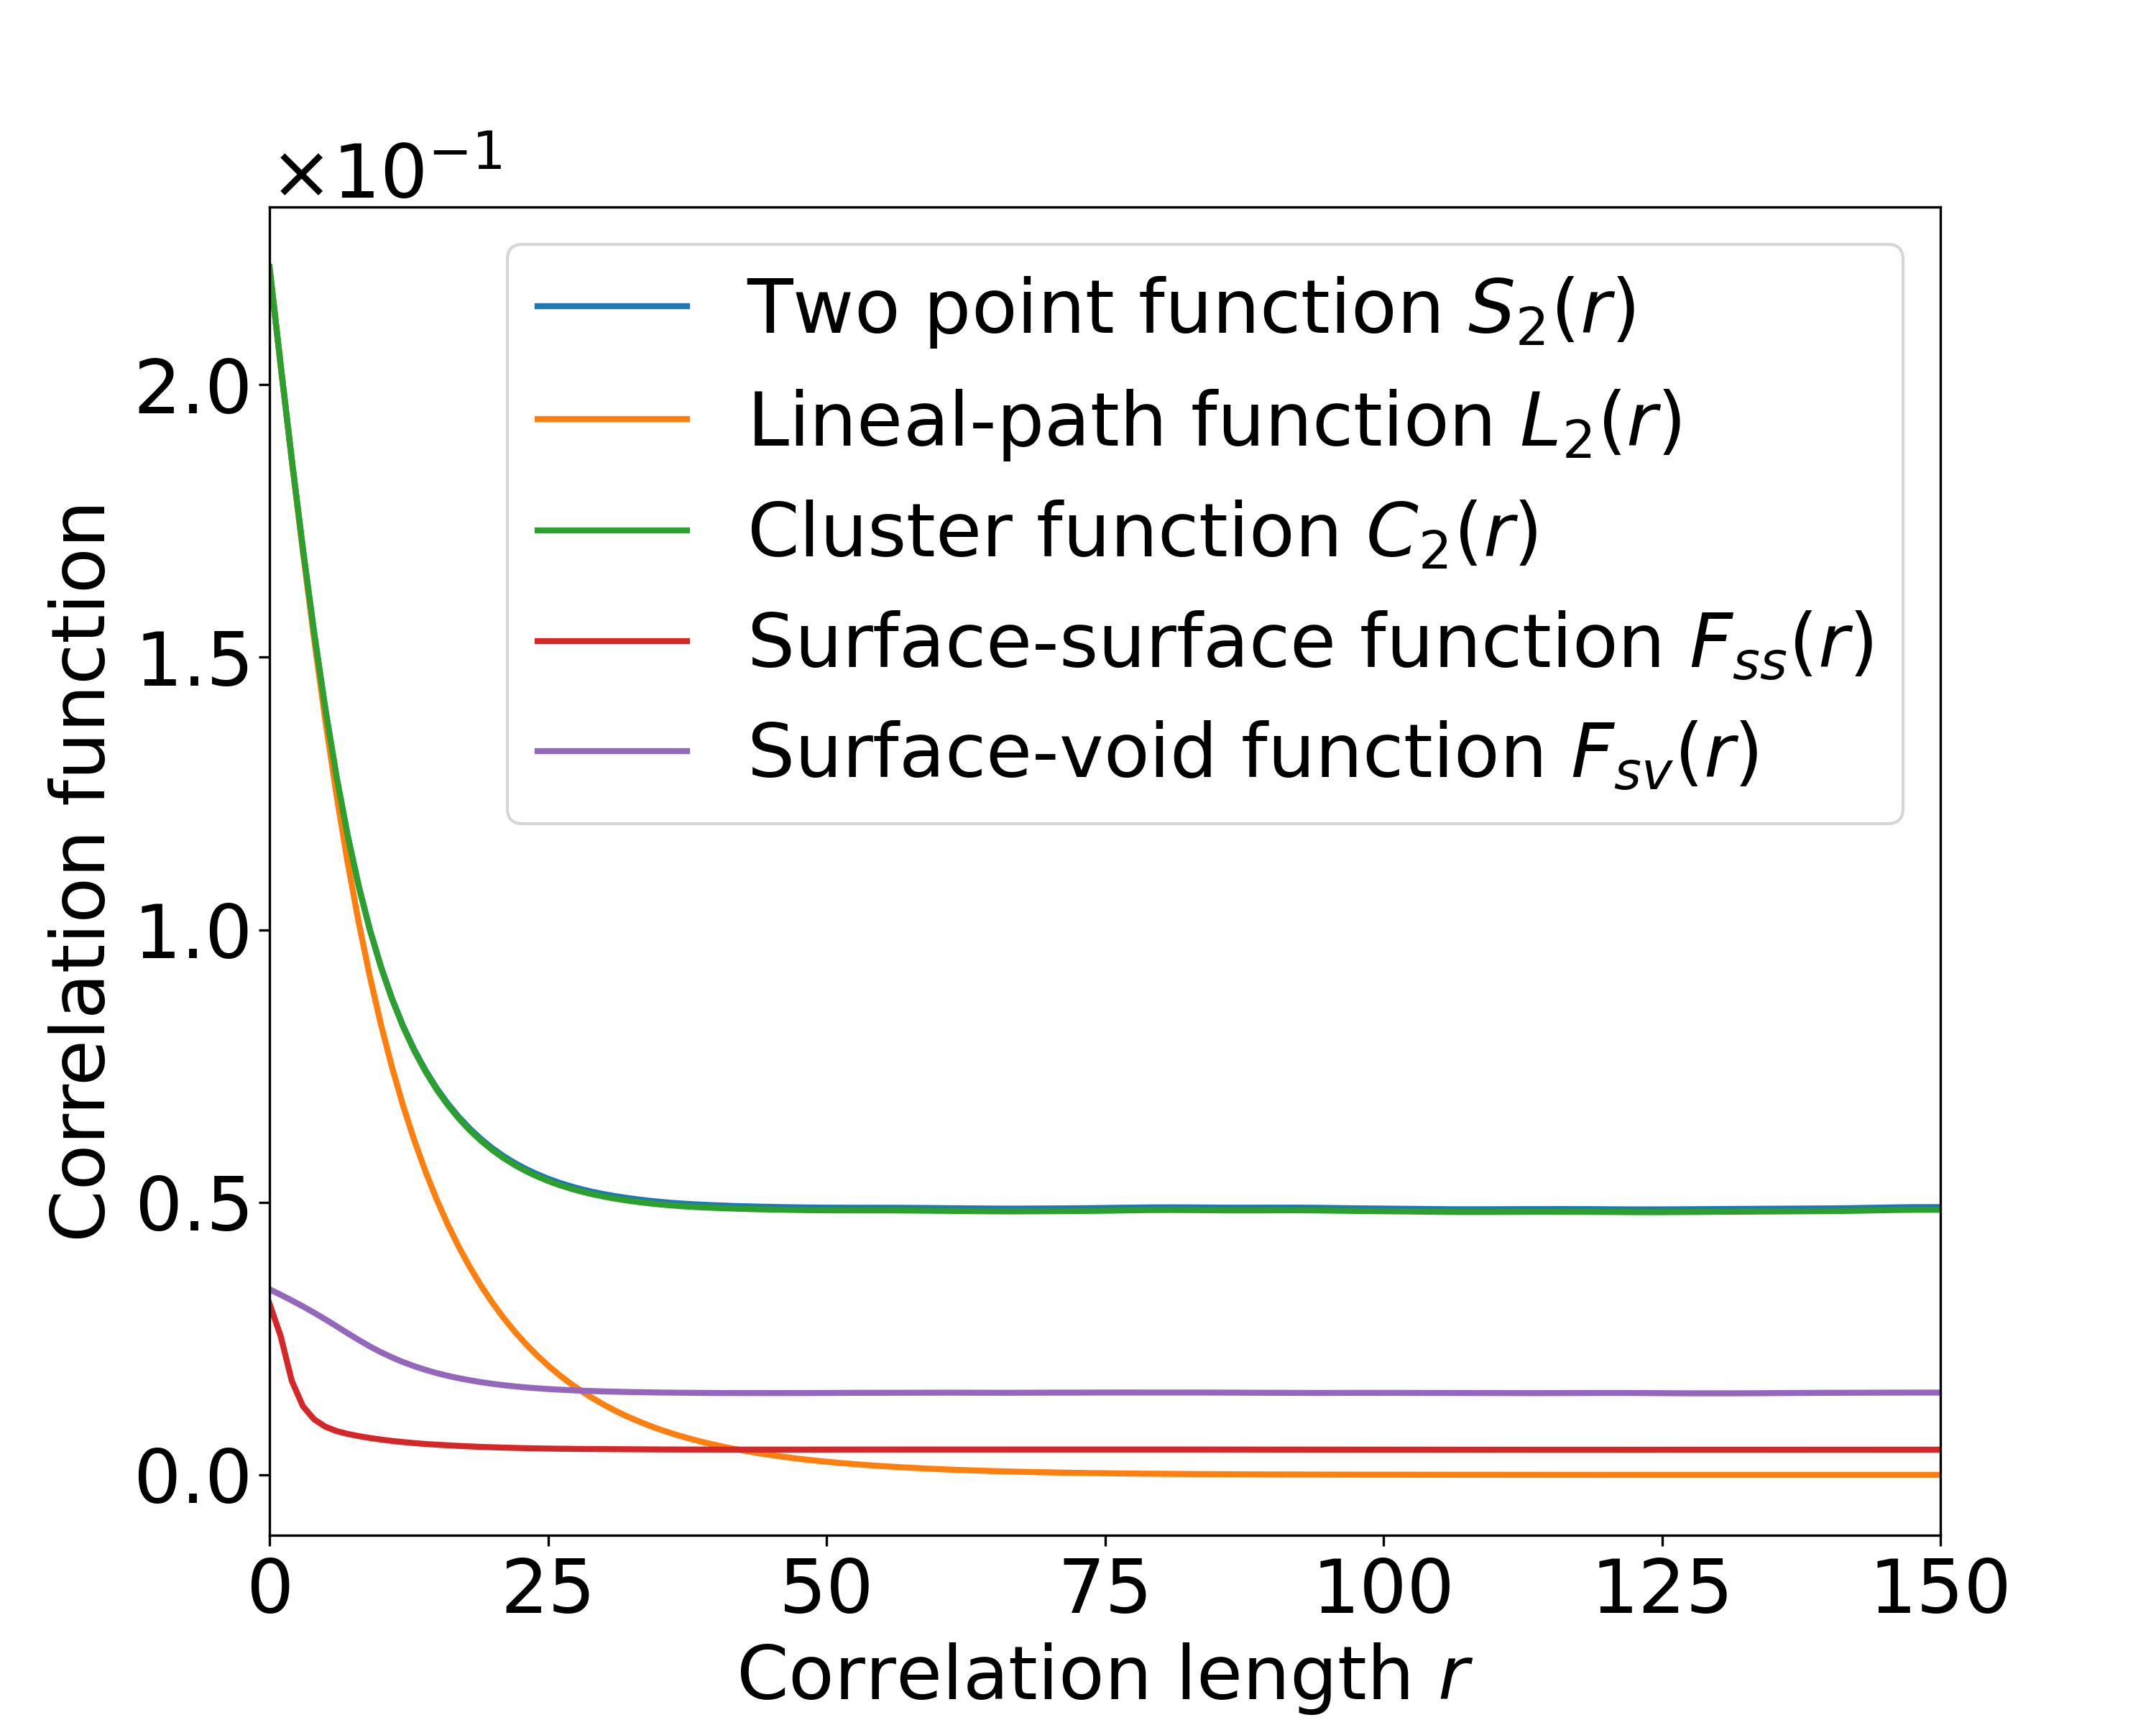
\includegraphics[width=0.3\linewidth]{real-data/Kirby_2d25um_binary-plot.png}
    \label{fig:kirby-plt}}
  \vskip\baselineskip
  \subfigure[Sandstone 1]{
    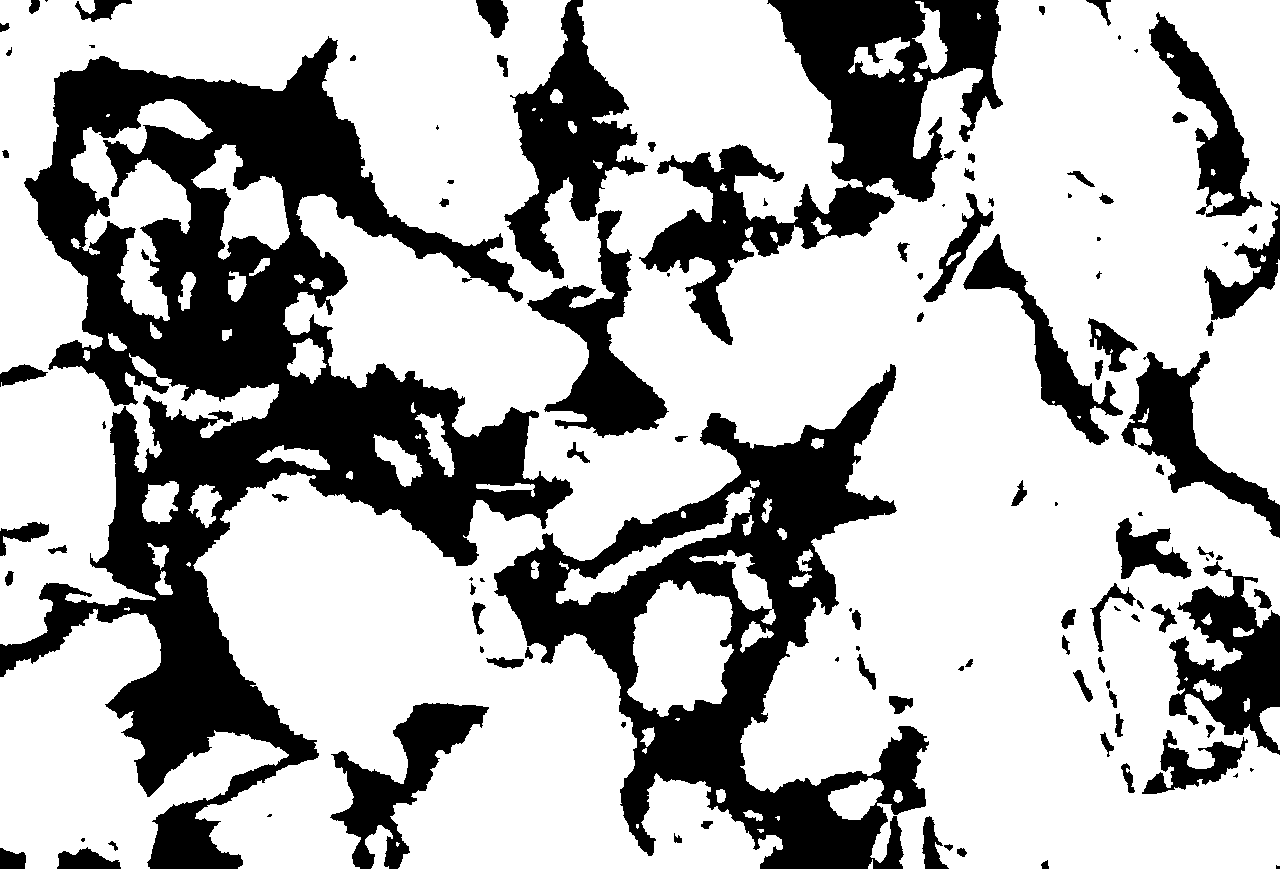
\includegraphics[width=0.3\linewidth]{real-data/sandstone1.png}
    \label{fig:real-sandstone-1}}
  \hfill
  \subfigure[Sandstone 2]{
    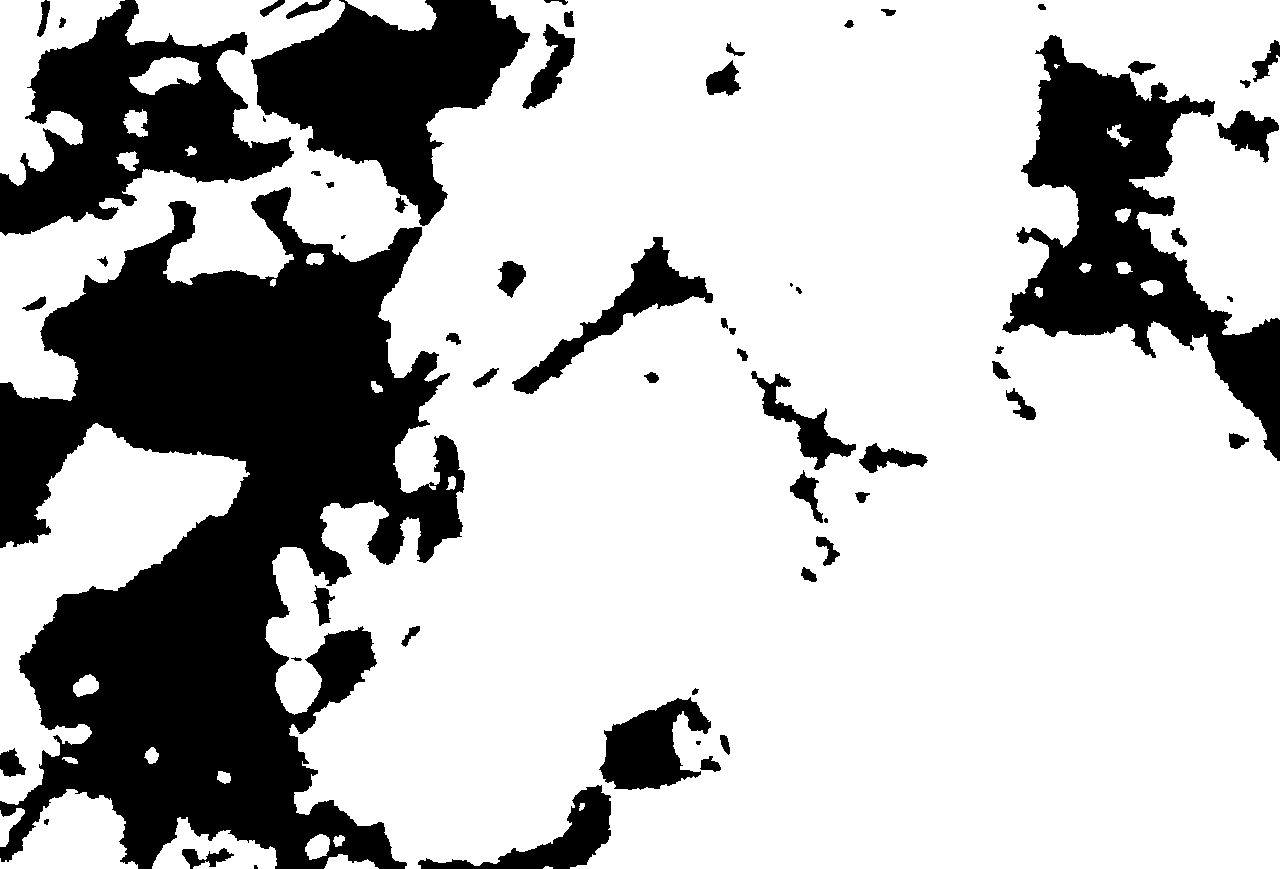
\includegraphics[width=0.3\linewidth]{real-data/sandstone2.png}
    \label{fig:real-sandstone-2}}
  \hfill
  \subfigure[Carbonate 1]{
    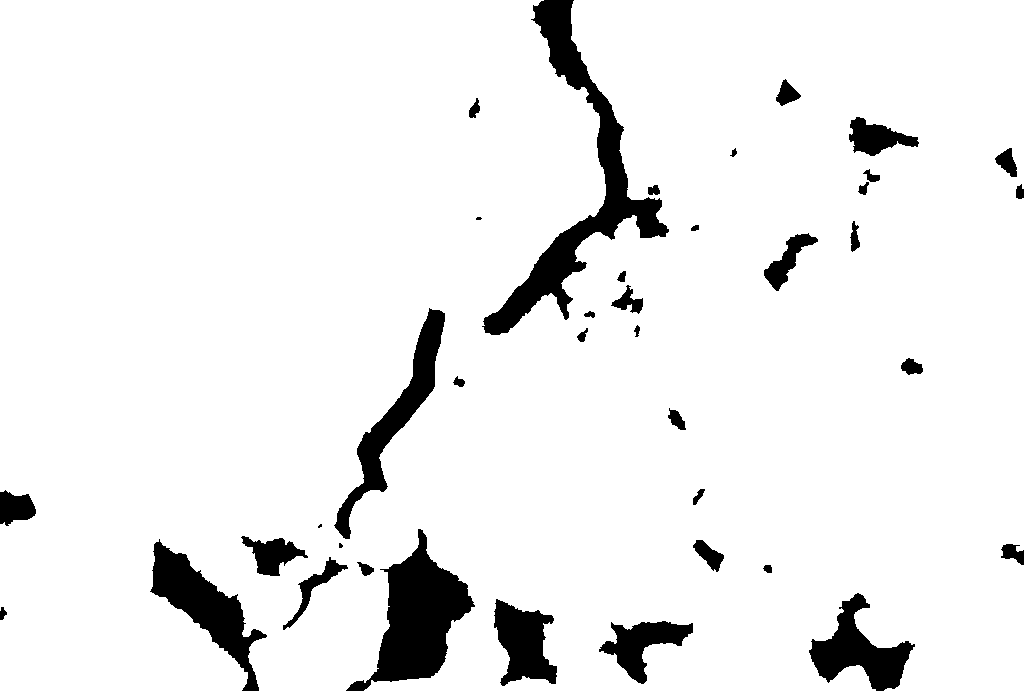
\includegraphics[width=0.3\linewidth]{real-data/carbonate1.png}
    \label{fig:real-carbonate-1-plt}}
  \vskip\baselineskip
  \subfigure[Sandstone 1 (correlation functions)]{
    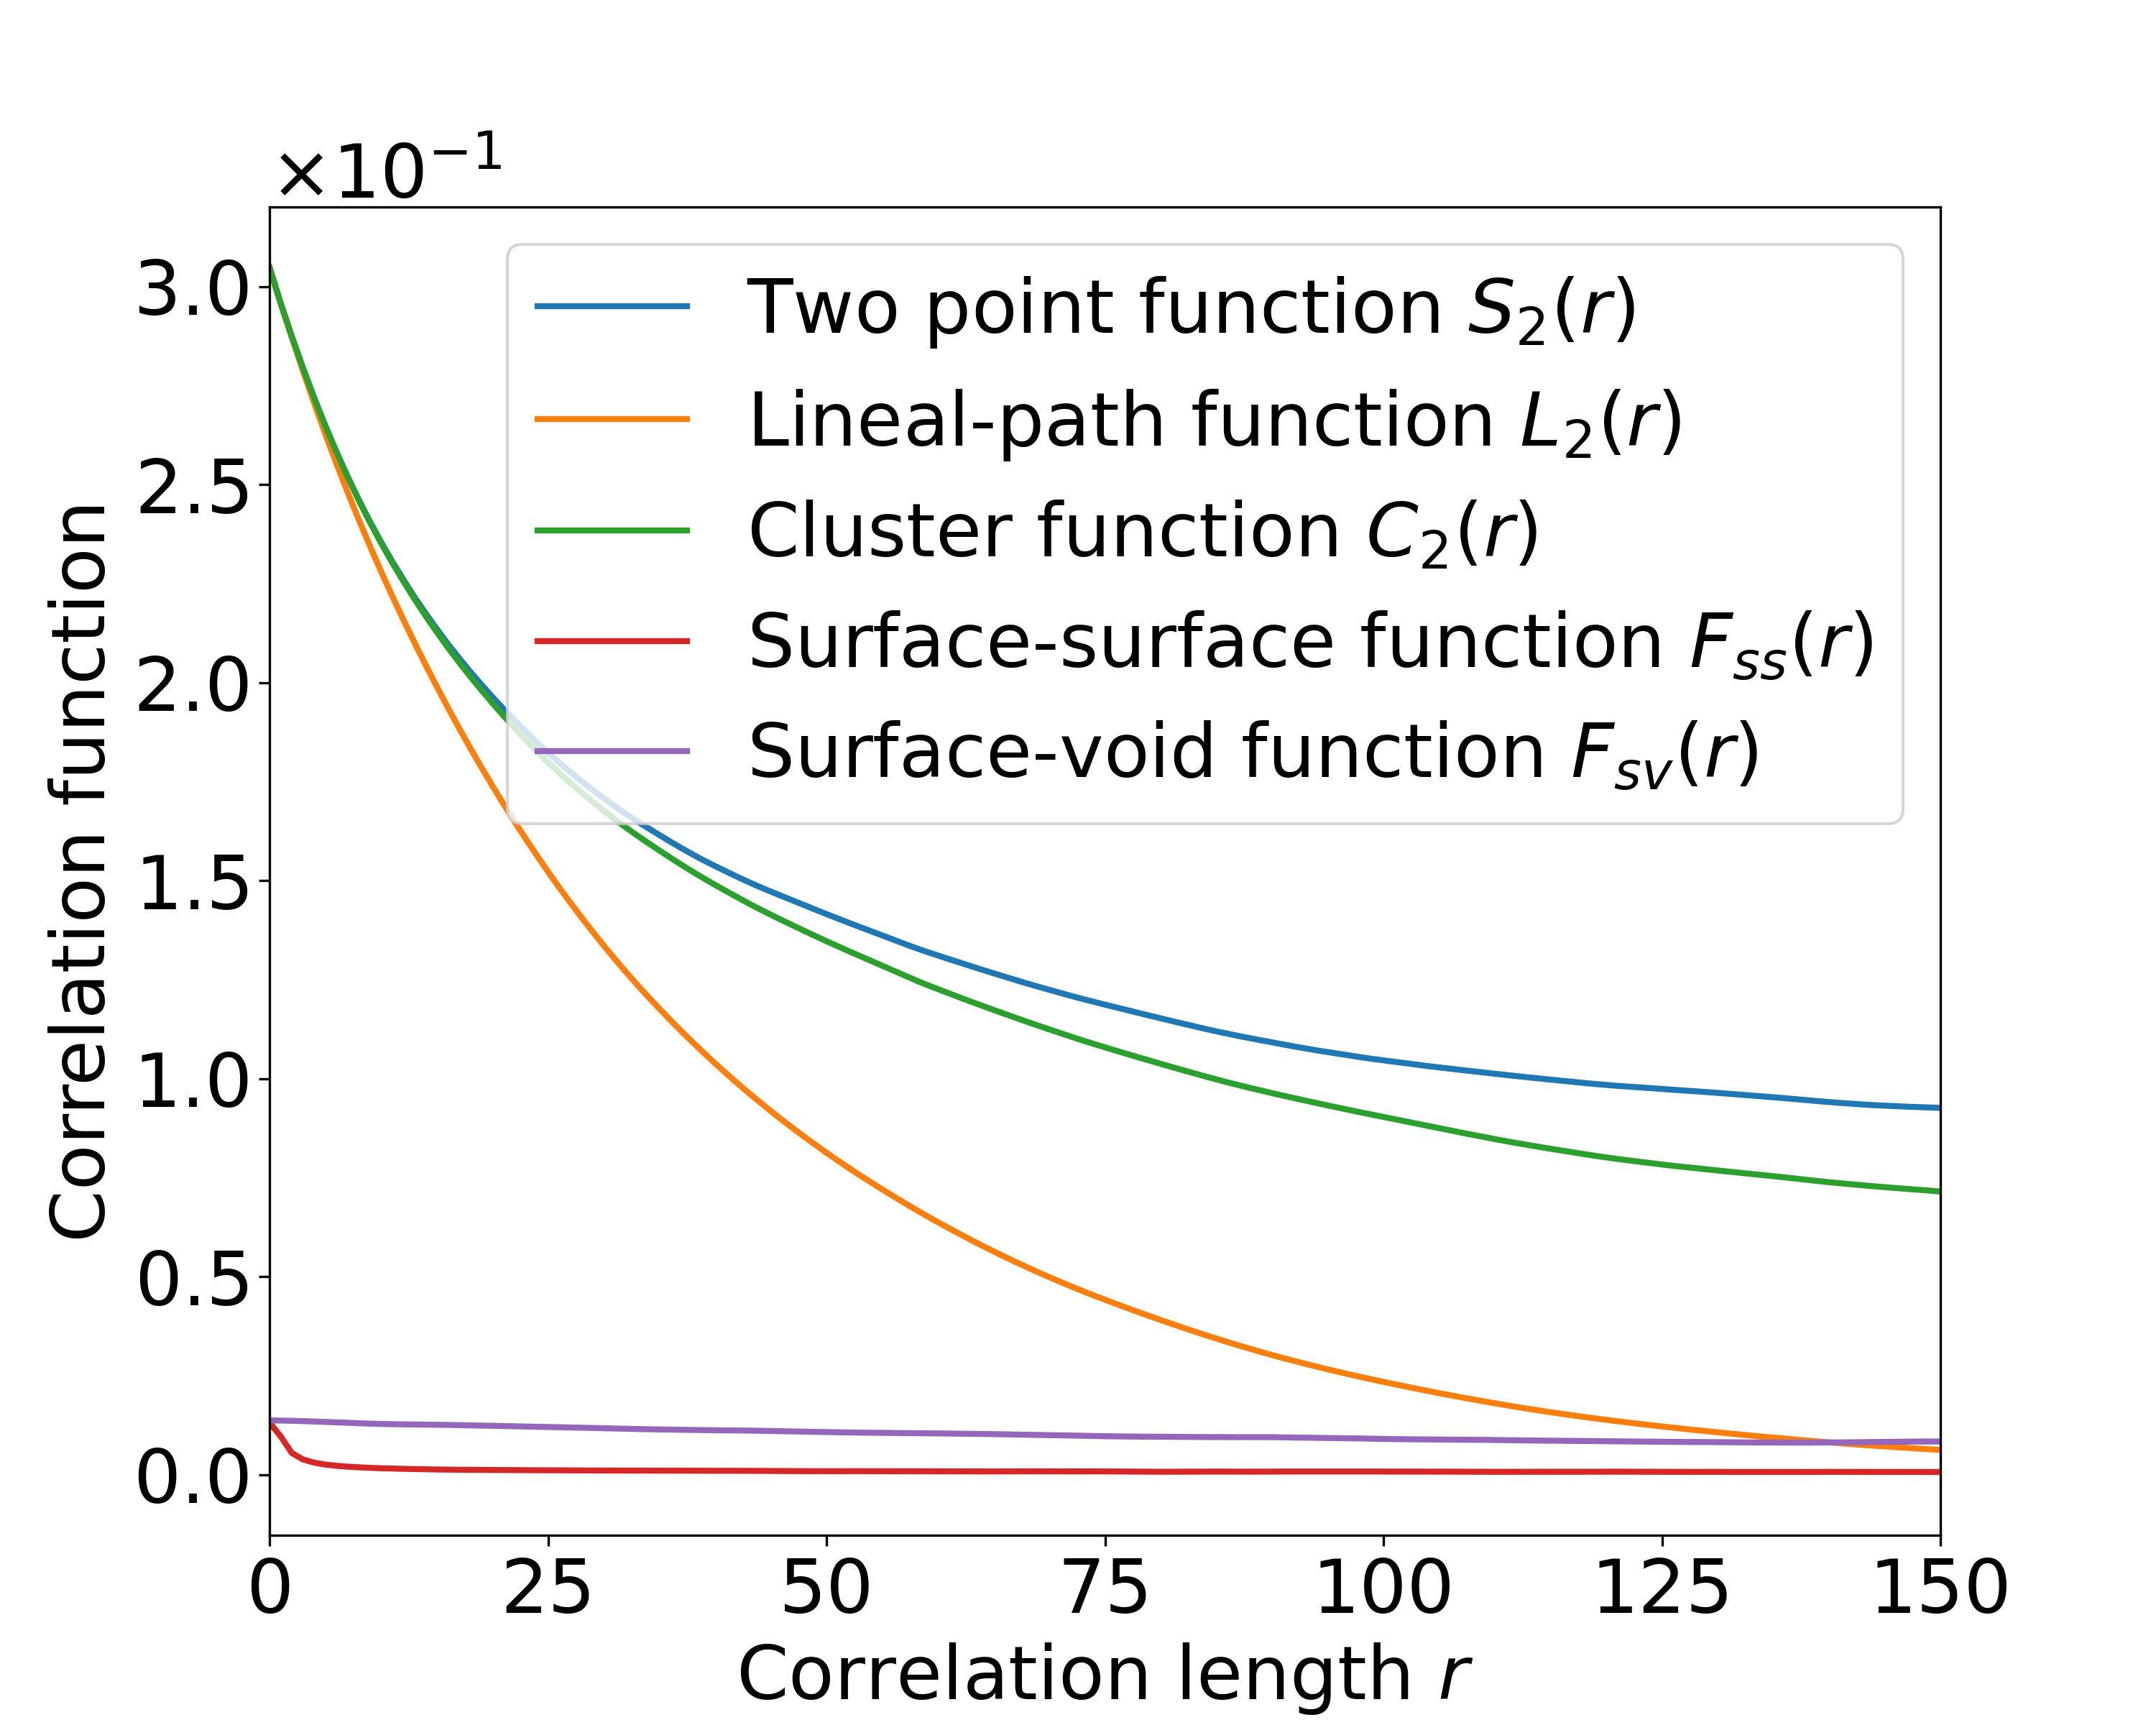
\includegraphics[width=0.3\linewidth]{real-data/sandstone1-plot.png}
    \label{fig:real-sandstone-1-plt}}
  \hfill
  \subfigure[Sandstone 2 (correlation functions)]{
    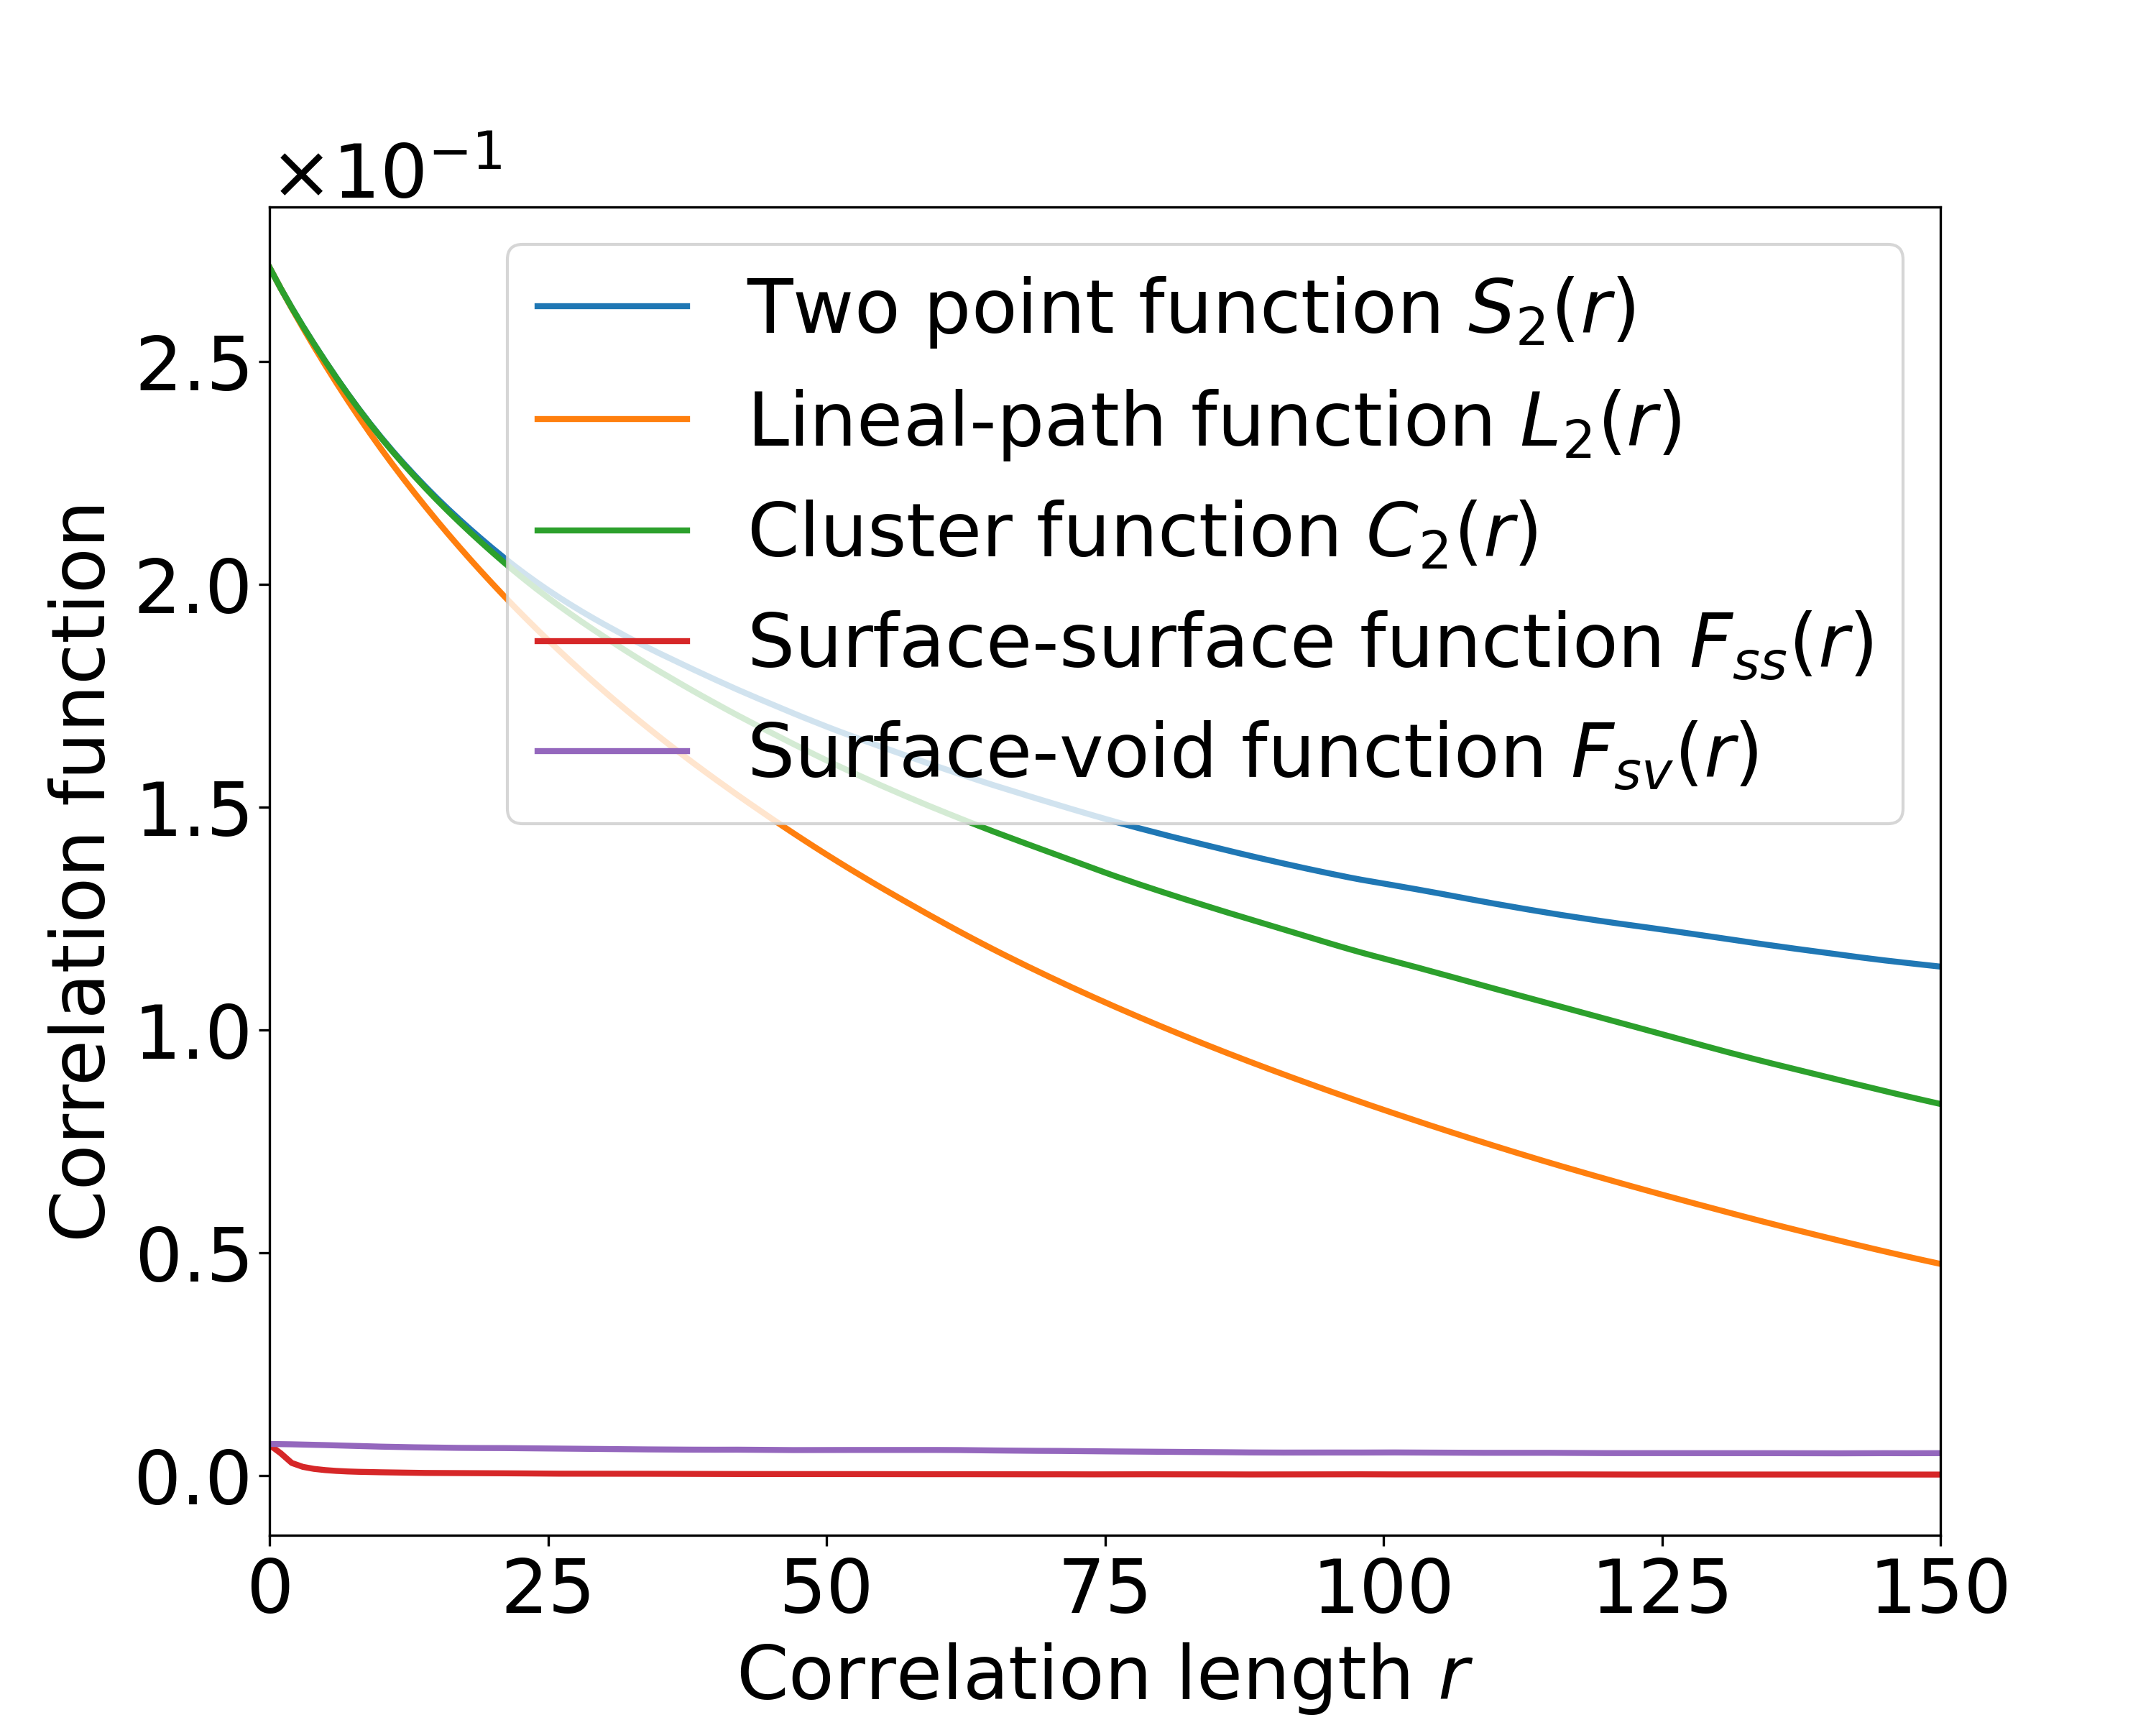
\includegraphics[width=0.3\linewidth]{real-data/sandstone2-plot.png}
    \label{fig:real-sandstone-2-plt}}
  \hfill
  \subfigure[Carbonate 1 (correlation functions)]{
    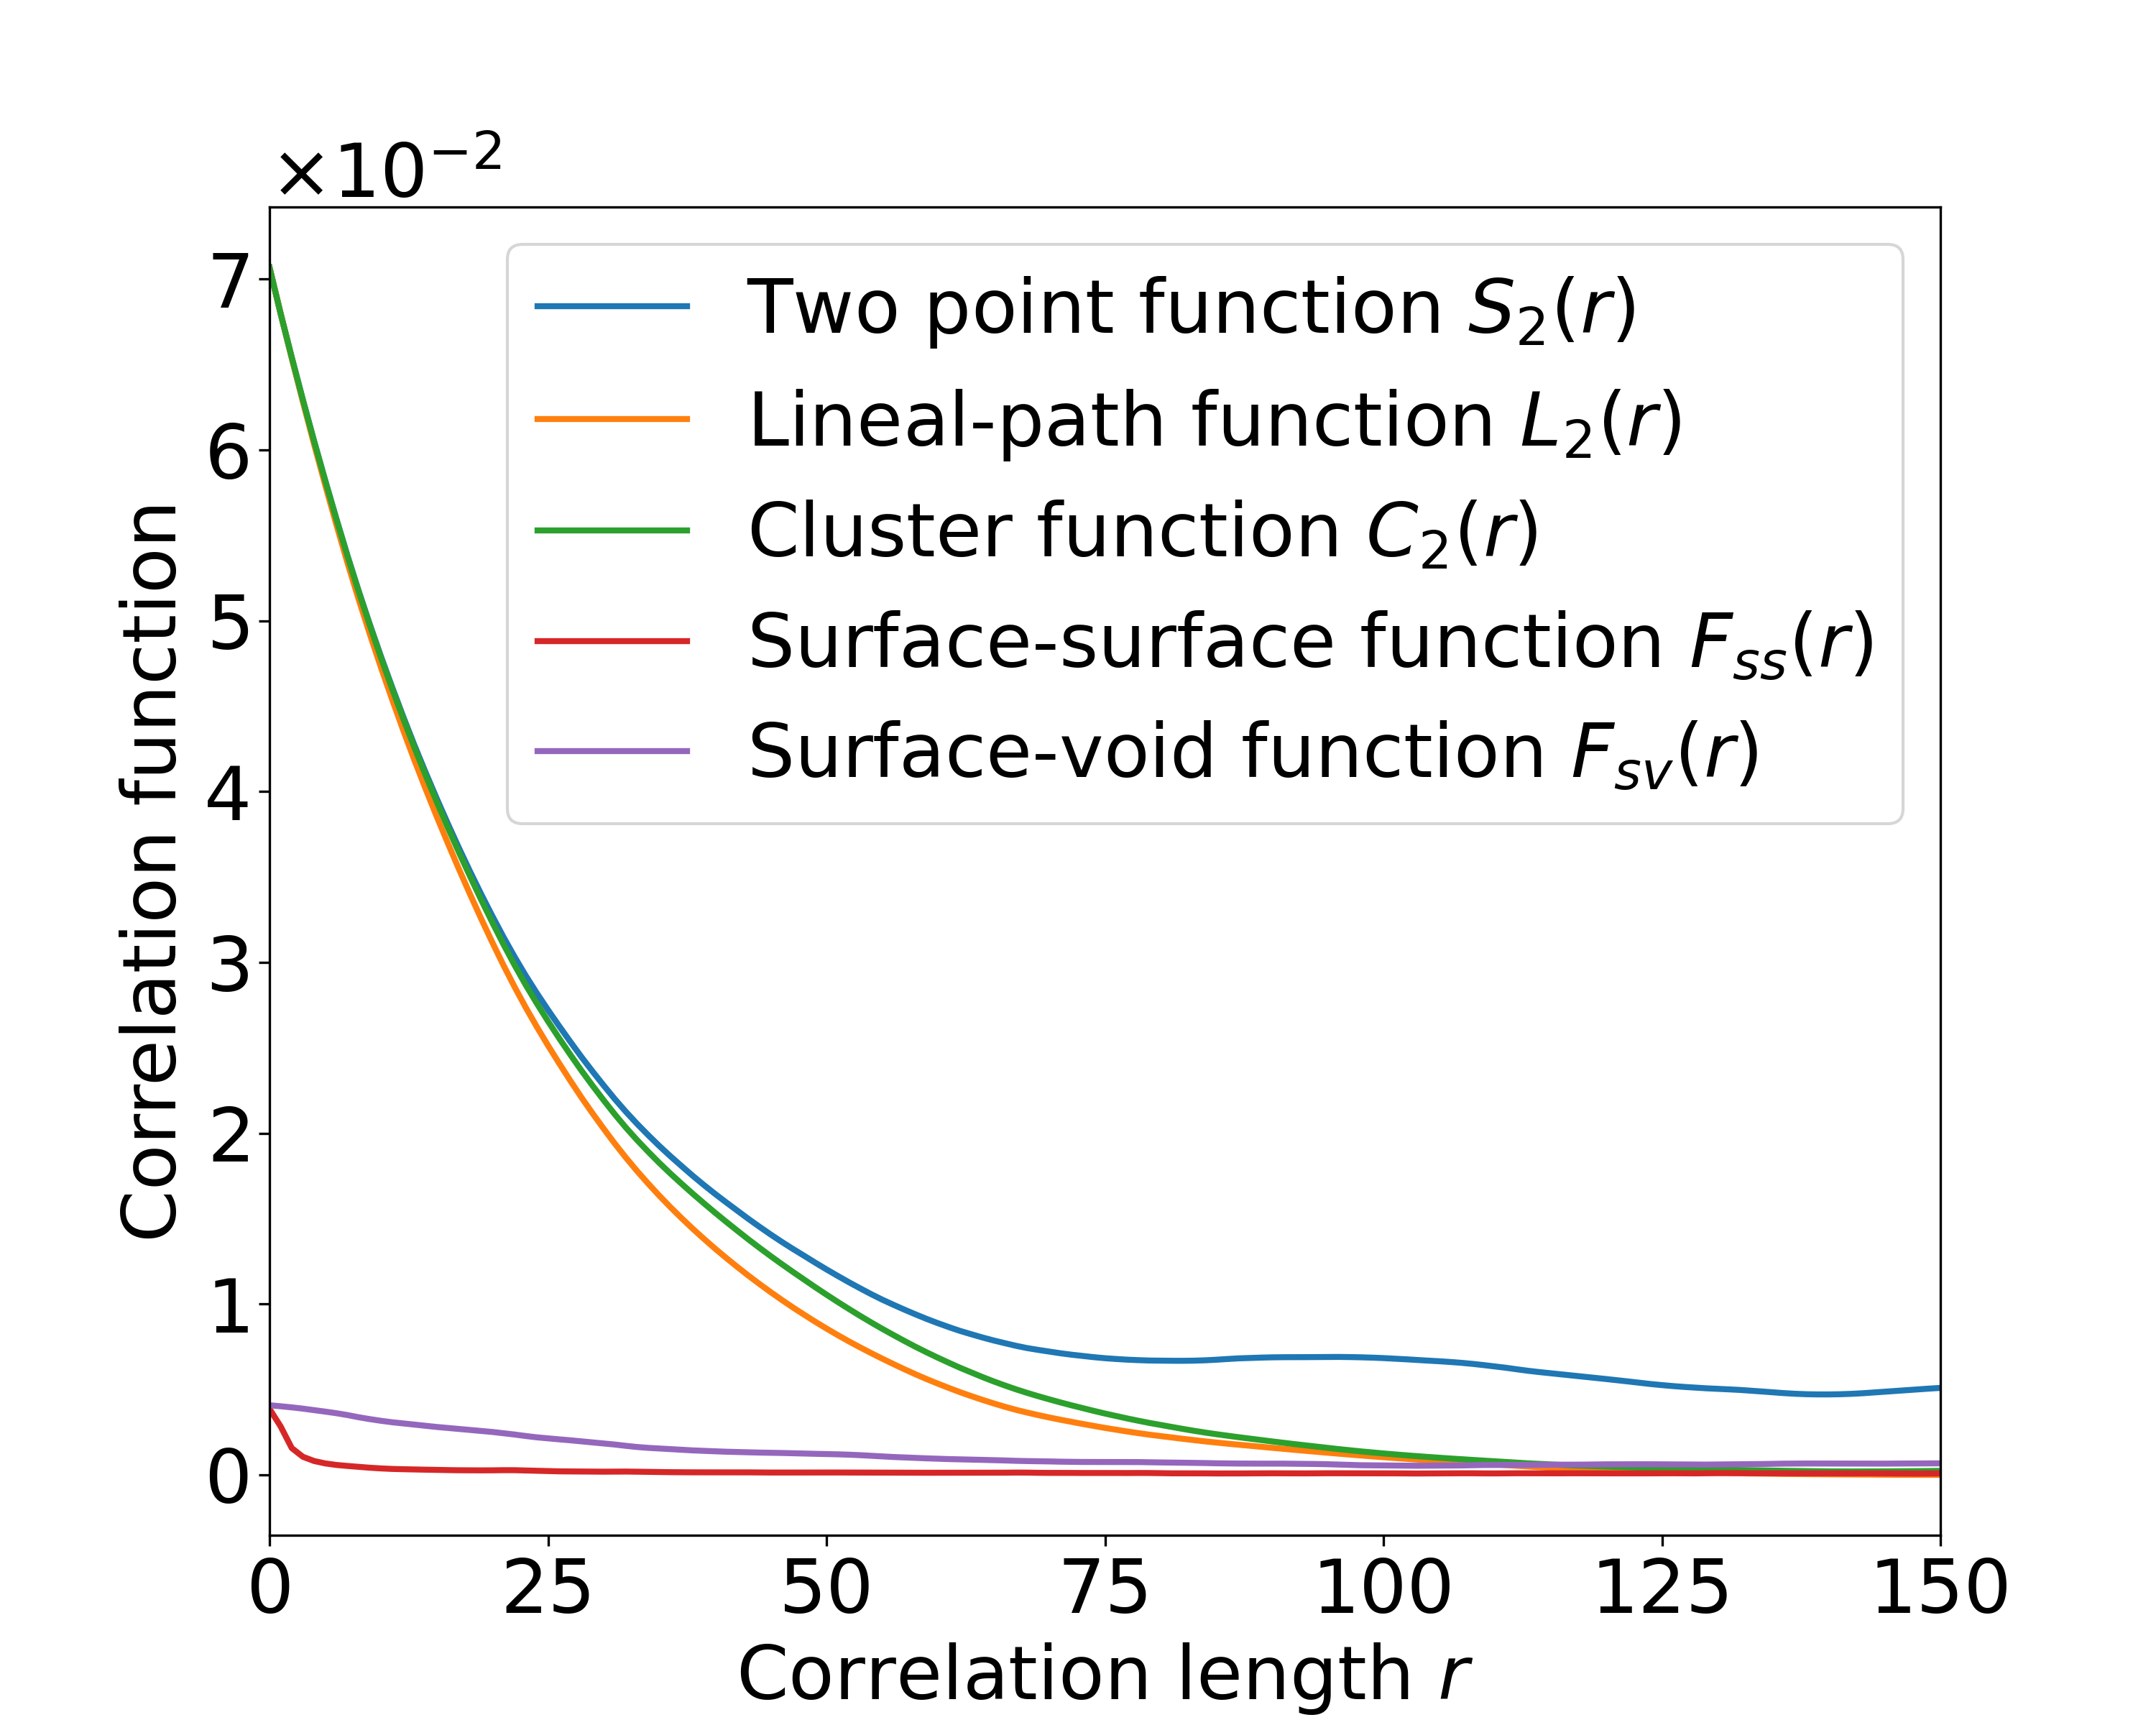
\includegraphics[width=0.3\linewidth]{real-data/carbonate1-plot.png}
    \label{fig:real-carbonate-1}}
  \caption[]{Plots of correlation functions for real samples.}
  \label{fig:real-data}
\end{figure*}

\section{Execution times of our algorithms}
\label{sec:efficiency}
To measure execution times of our algorithms we use a machine with the following
configuration:\textcolor{red}{Must be configuration of Asus notebook}
\begin{itemize}
\item \textbf{CPU}: AMD Ryzen 5 1600X
\item \textbf{Memory}: 32~Gb DDR4-2400 memory
\item \textbf{GPU}: Nvidia Tesla V100 with 32~Gb video memory
\end{itemize}

We generate two (resp. three) dimensional square (resp. cubic) binary arrays
with different sides. An array used for measurements contains two solid disks
(resp. balls) surrounded by void phase, therefore it is excected for $C_2$
function to perform two times slower than $S_2$.

To measure efficiency of \code{Directional} module we generate ten arrays with
a side of a square $s = 1000, 2000, \dots, 10000$ pixels for two-dimensional
case and ten arrays with a side of a cube $s = 50, 100, \dots, 500$ voxels for
three-dimensional case and calculate execution time for each function. All
functions are calculated along axial directions using periodic boundary
conditions.

With the \code{Map} module we follow the same procedure. Many functions in
\code{Map} can utilize Nvidia's GPUs using the CUDA library. For example,
two-point correlation function uses FFT transform optimized for Nvidia GPUs and
provided in \code{CUDA.FFT} package. We provide execution times for both CPU and
GPU. The choice between CPU or GPU version is made depending on type of input
array. If it's \code{CuArray} rather than generic \code{AbstractArray} then CUDA
implementation is chosen. \textcolor{red}{Please note, that CPU versions are
  much slower, so we choose a different sides of squares
  ($s = 700, 1350, \dots, 7000$) and cubes ($s = 10, 45, \dots, 350$)
  for evaluation of the performance.}

The measurements of execution time is on \cref{fig:timings}. As you can see, GPU
versions (when available) are faster than CPU versions and limited only by
amount of video memory. Functions in \code{Directional} are the slowest among
other implementations, but require less memory.

% Replace by two disks?
\begin{figure}[ht]
  \centering
  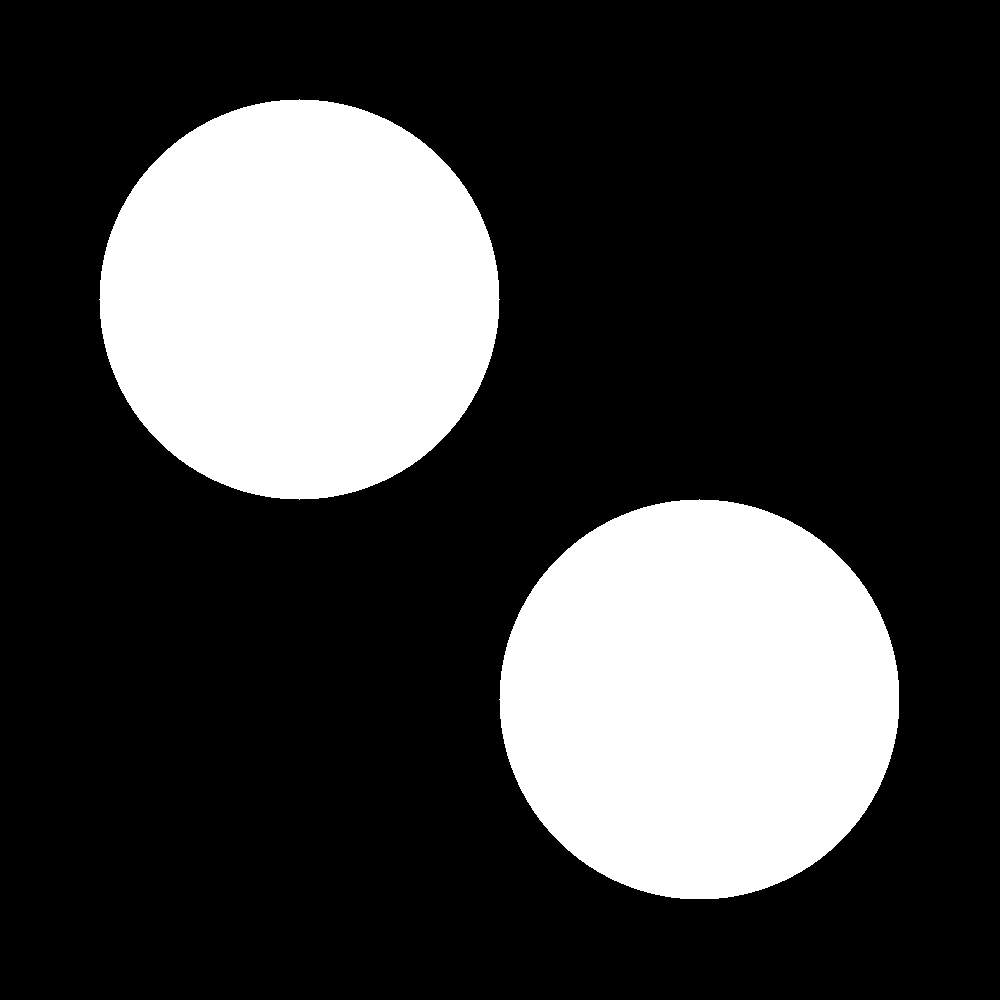
\includegraphics[width=0.6\linewidth]{images/timing-image.png}
  \caption[]{One of 2D image used in timing measurements.}
  \label{fig:valuenoise}
\end{figure}

\begin{figure*}[t]
  \centering
  \subfigure[Two-dimensional case, module \code{Directional}]{
    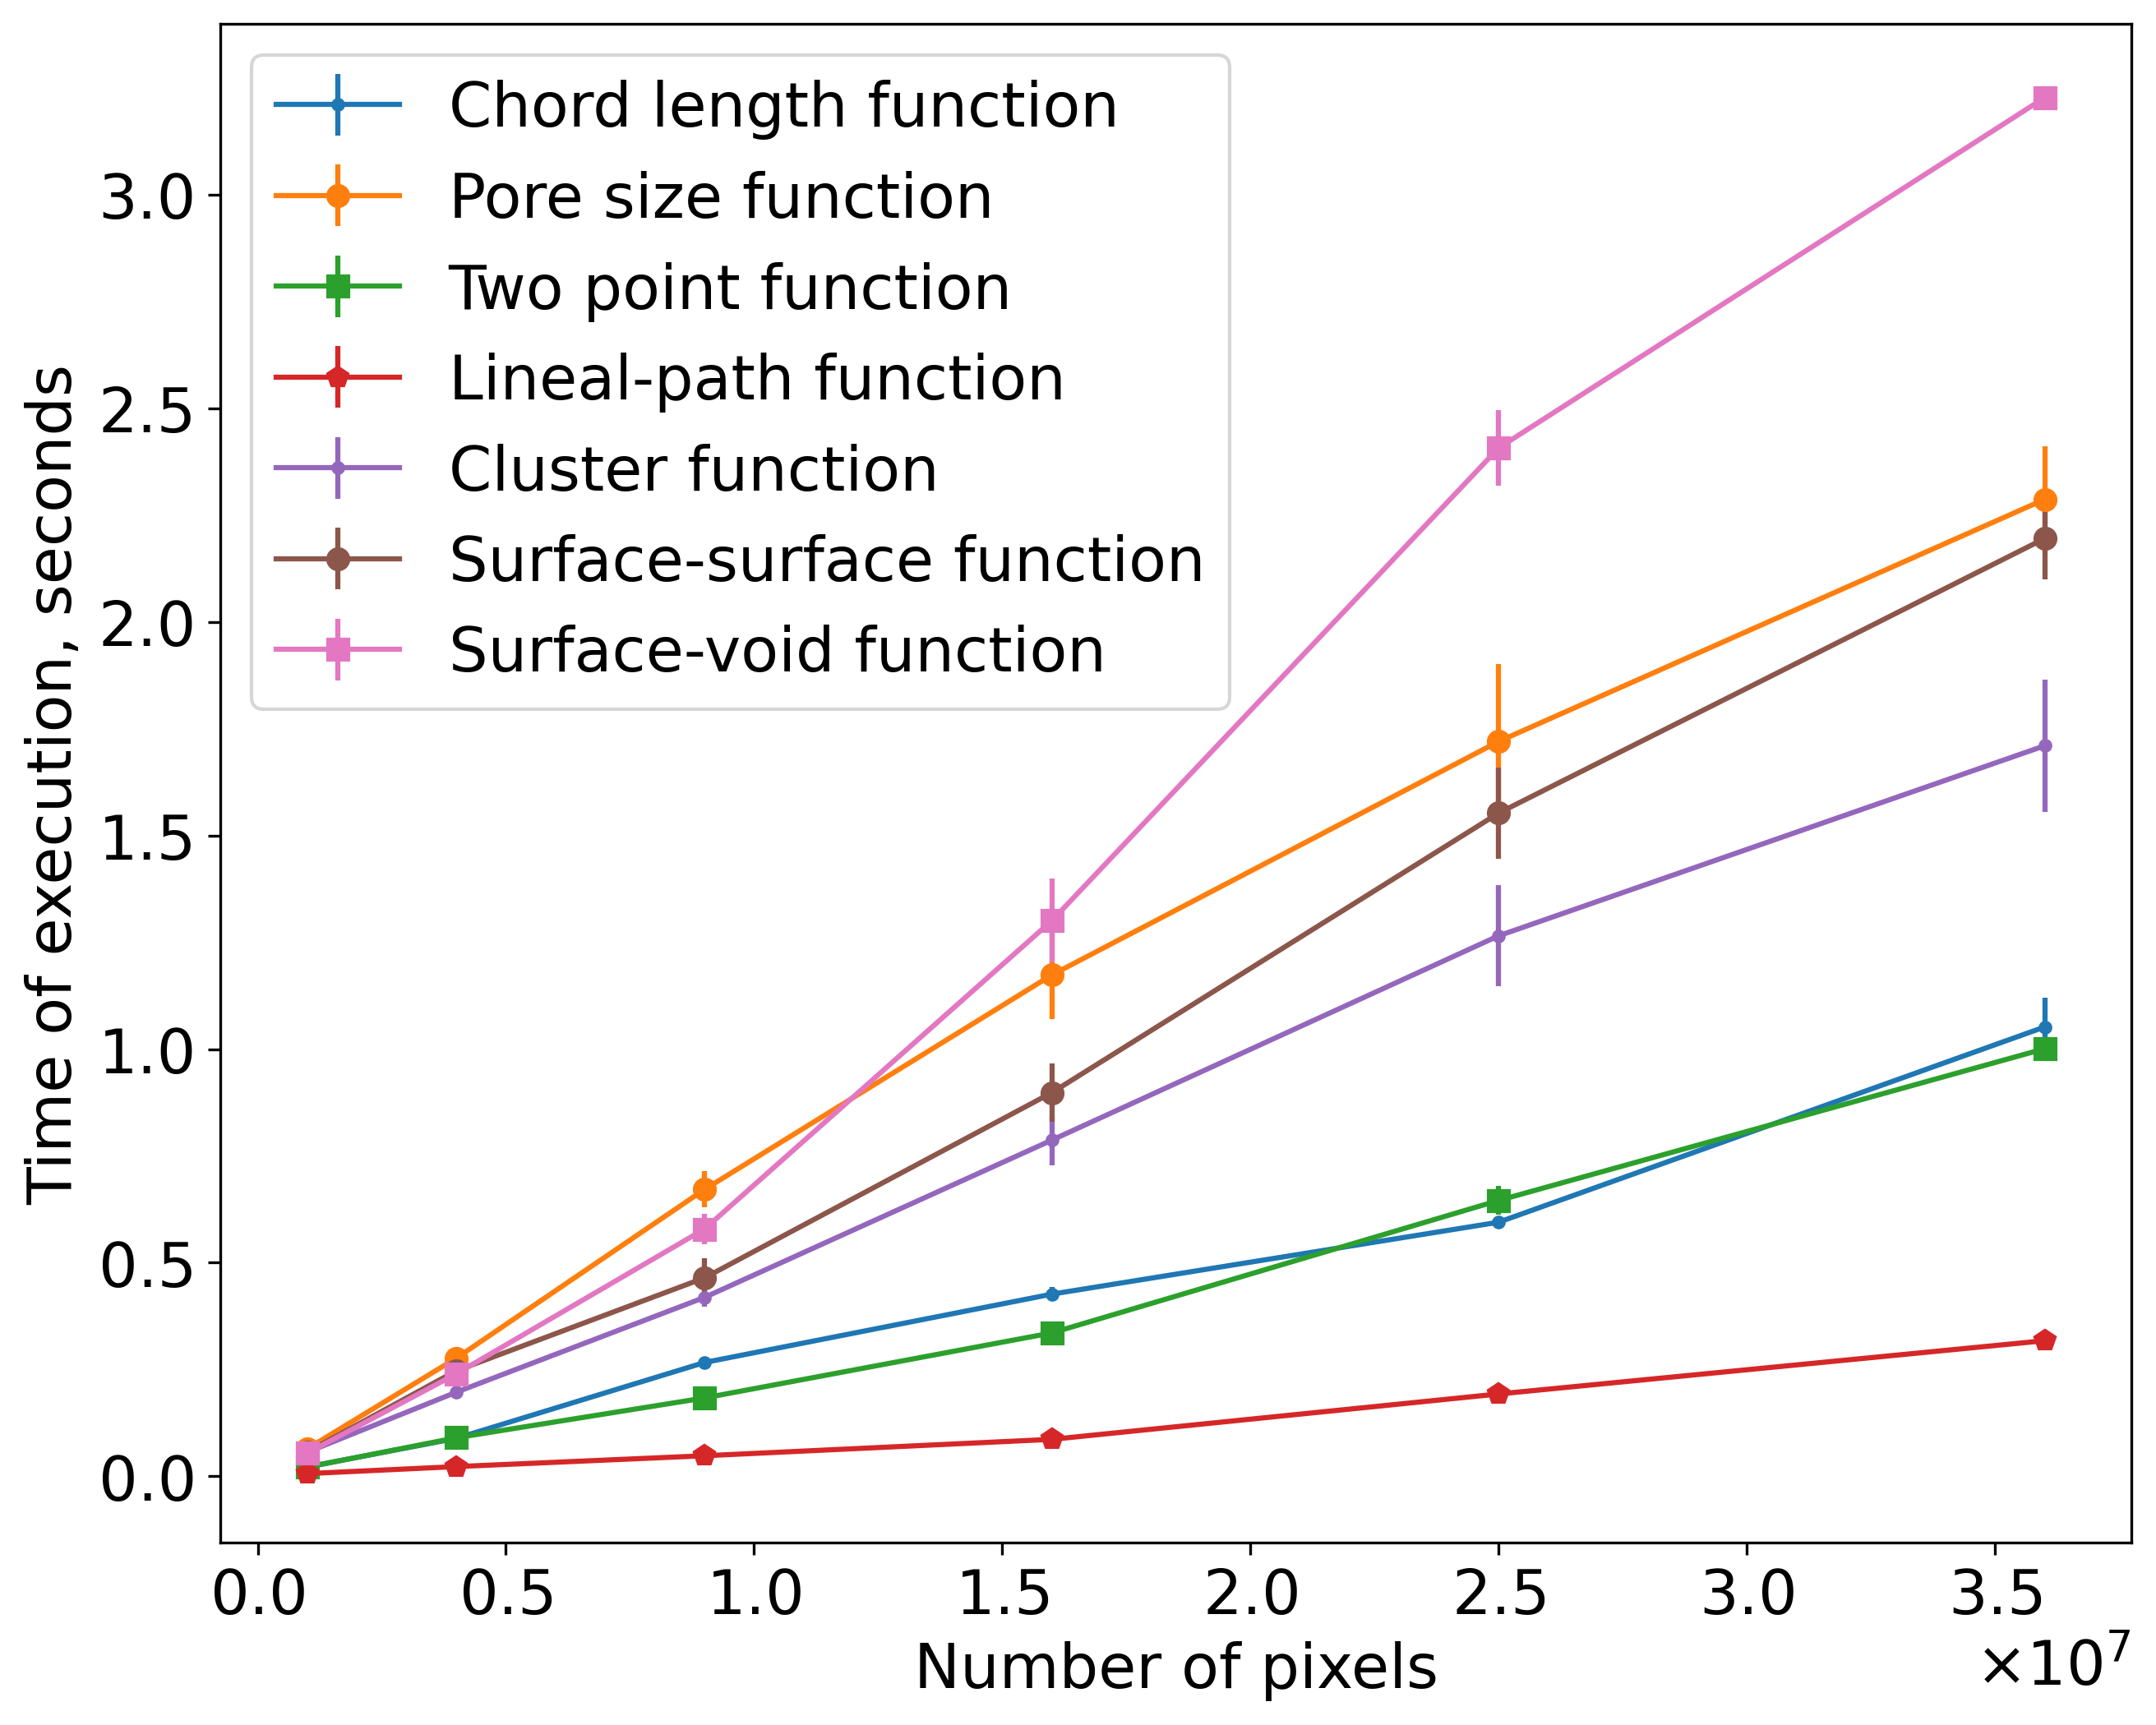
\includegraphics[width=0.475\linewidth]{images/time-2d.png}
    \label{fig:timings-2d}}
  \hfill
  \subfigure[Three-dimensional case, module \code{Directional}]{
    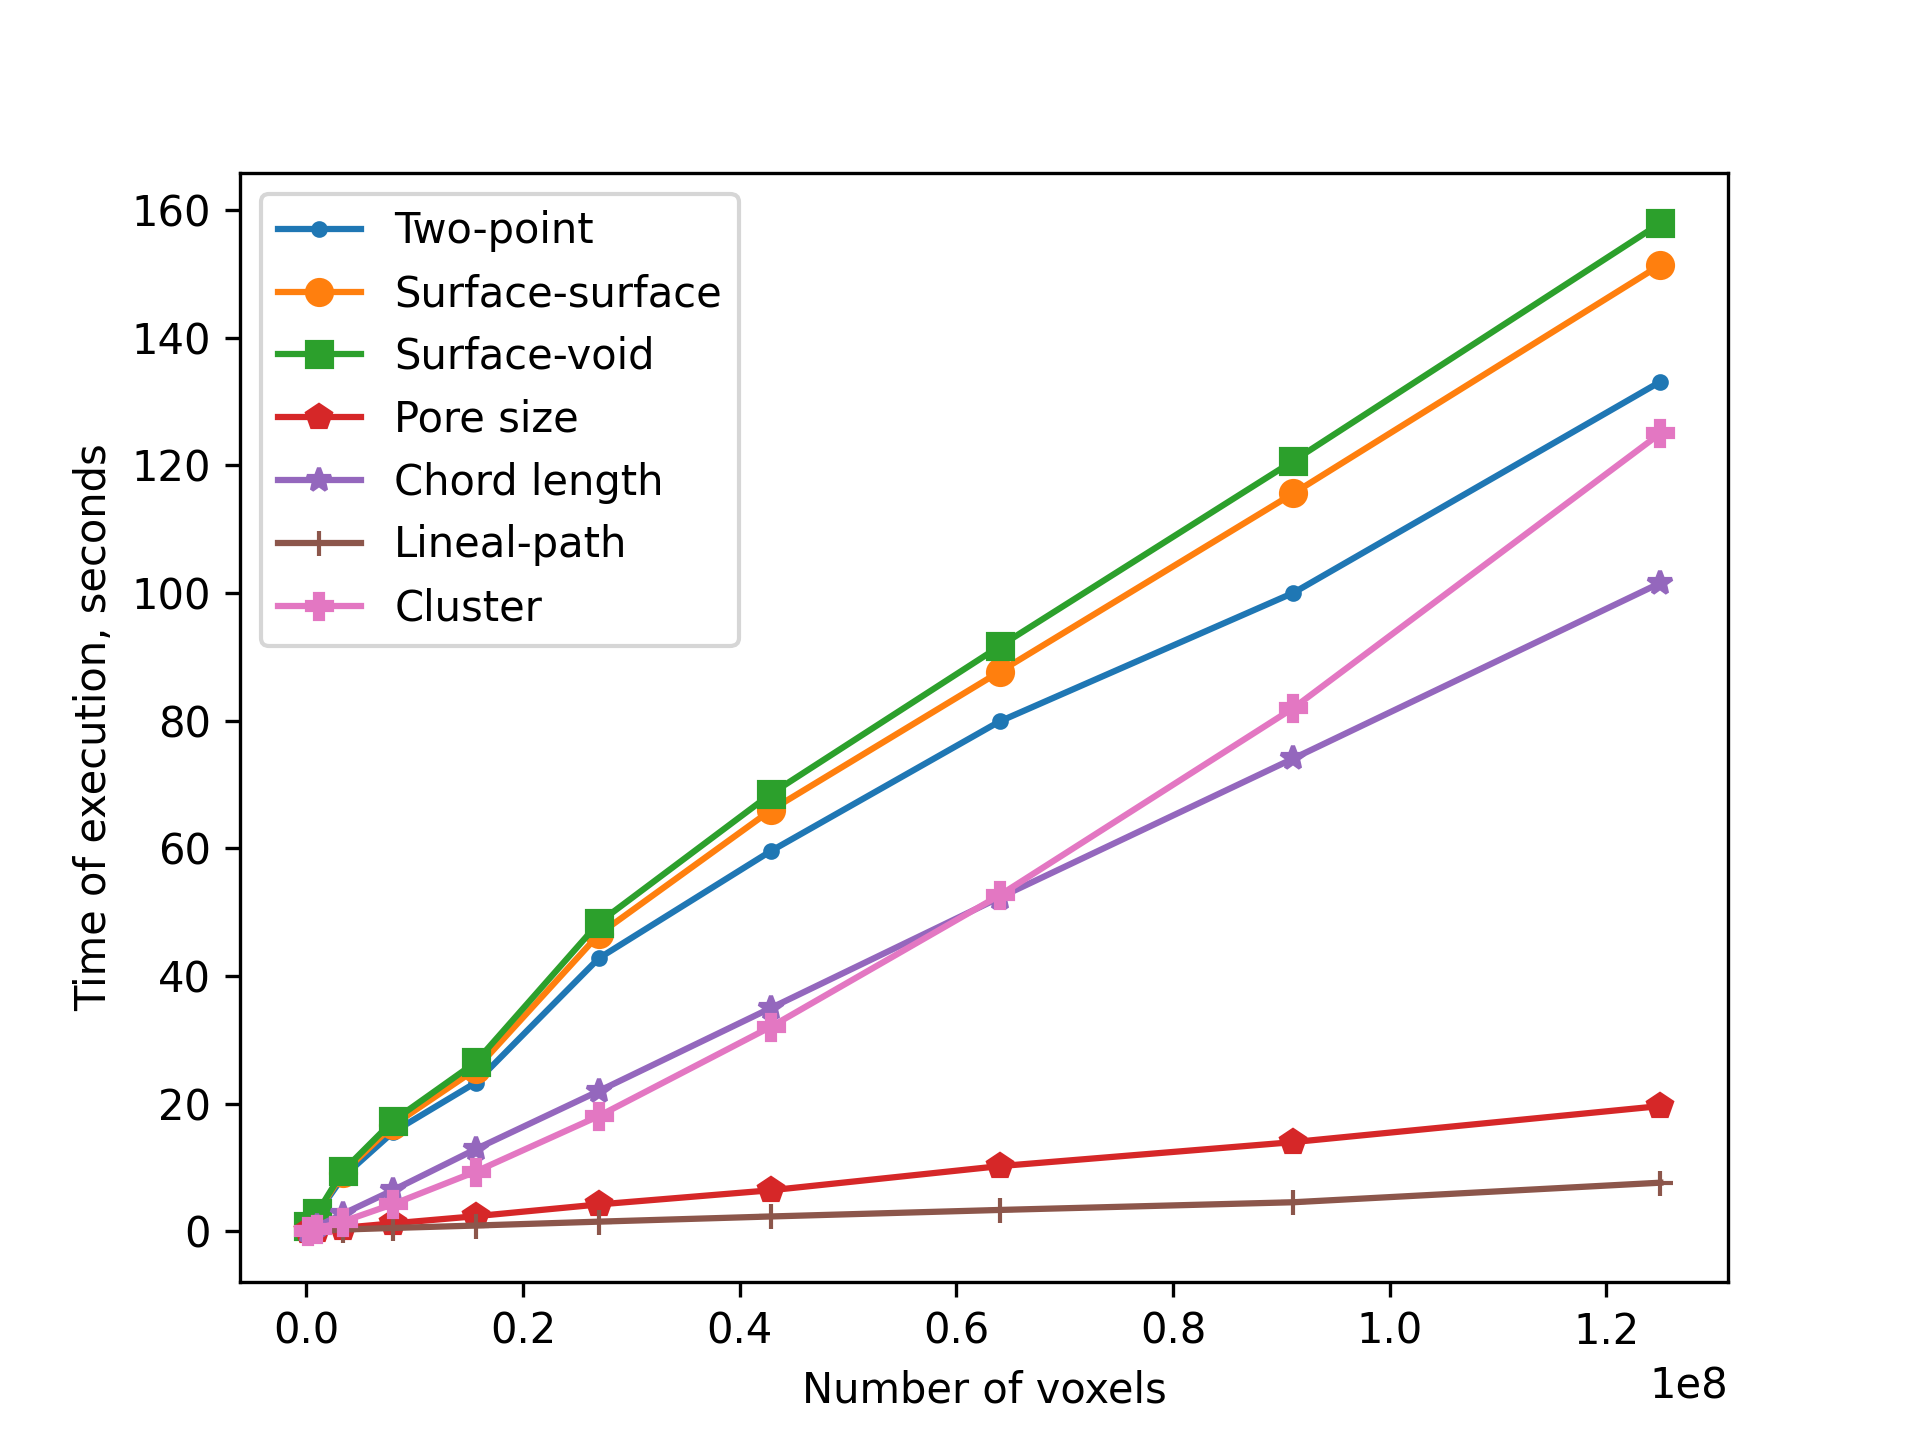
\includegraphics[width=0.475\linewidth]{images/time-3d.png}
    \label{fig:timings-3d}}
  \vskip\baselineskip
  \subfigure[Two-dimensional case, module \code{Map}, CPU]{
    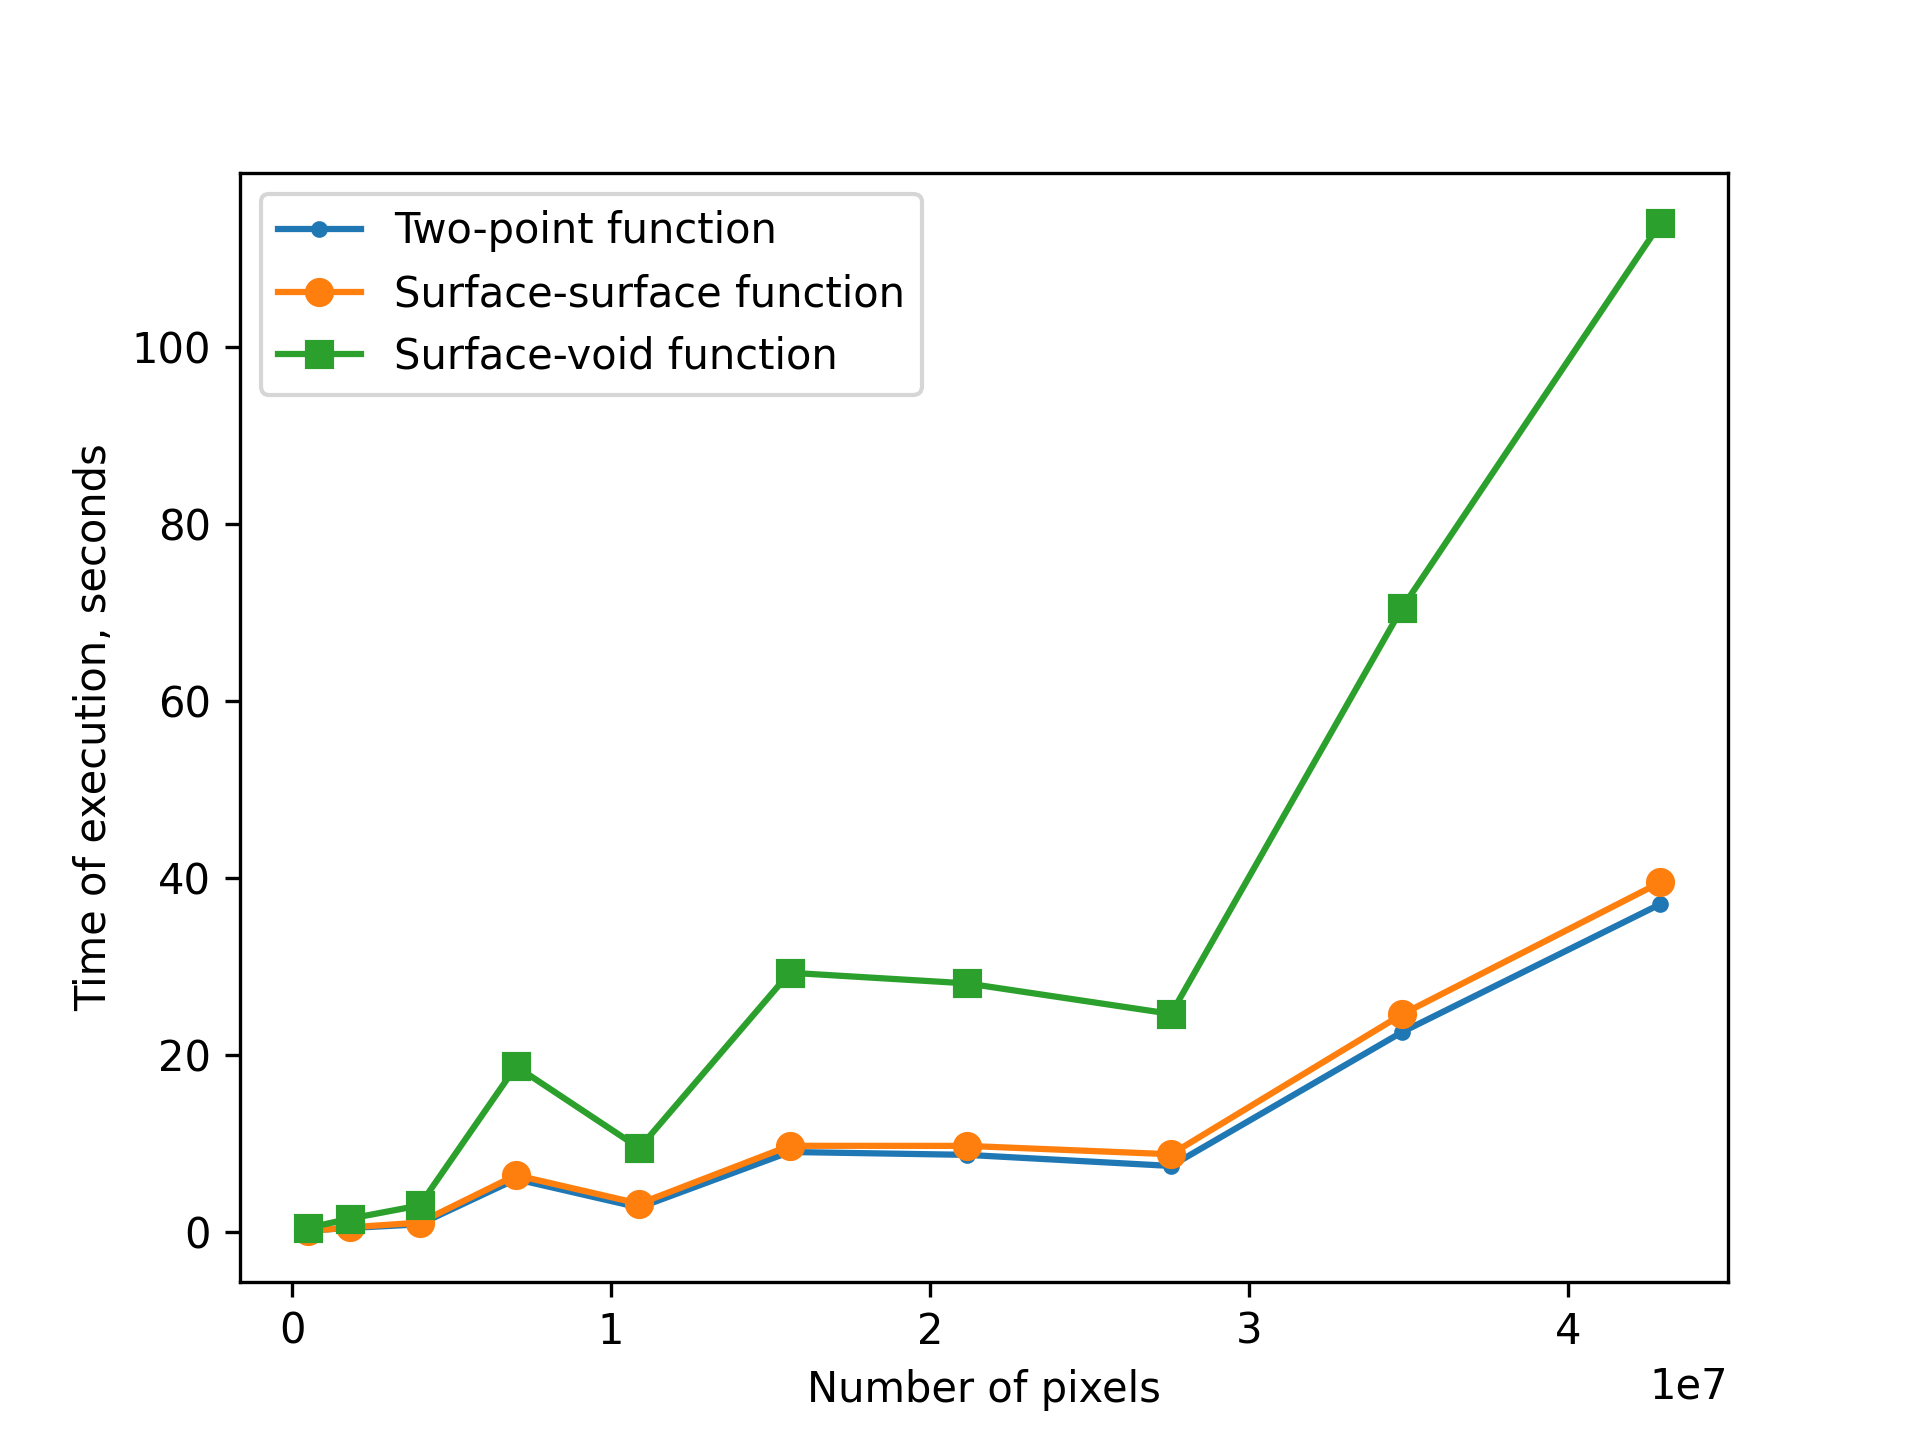
\includegraphics[width=0.475\linewidth]{images/time-2d-map.png}
    \label{fig:timings-2d-map}}
  \hfill
  \subfigure[Three-dimensional case, module \code{Map}, CPU]{
    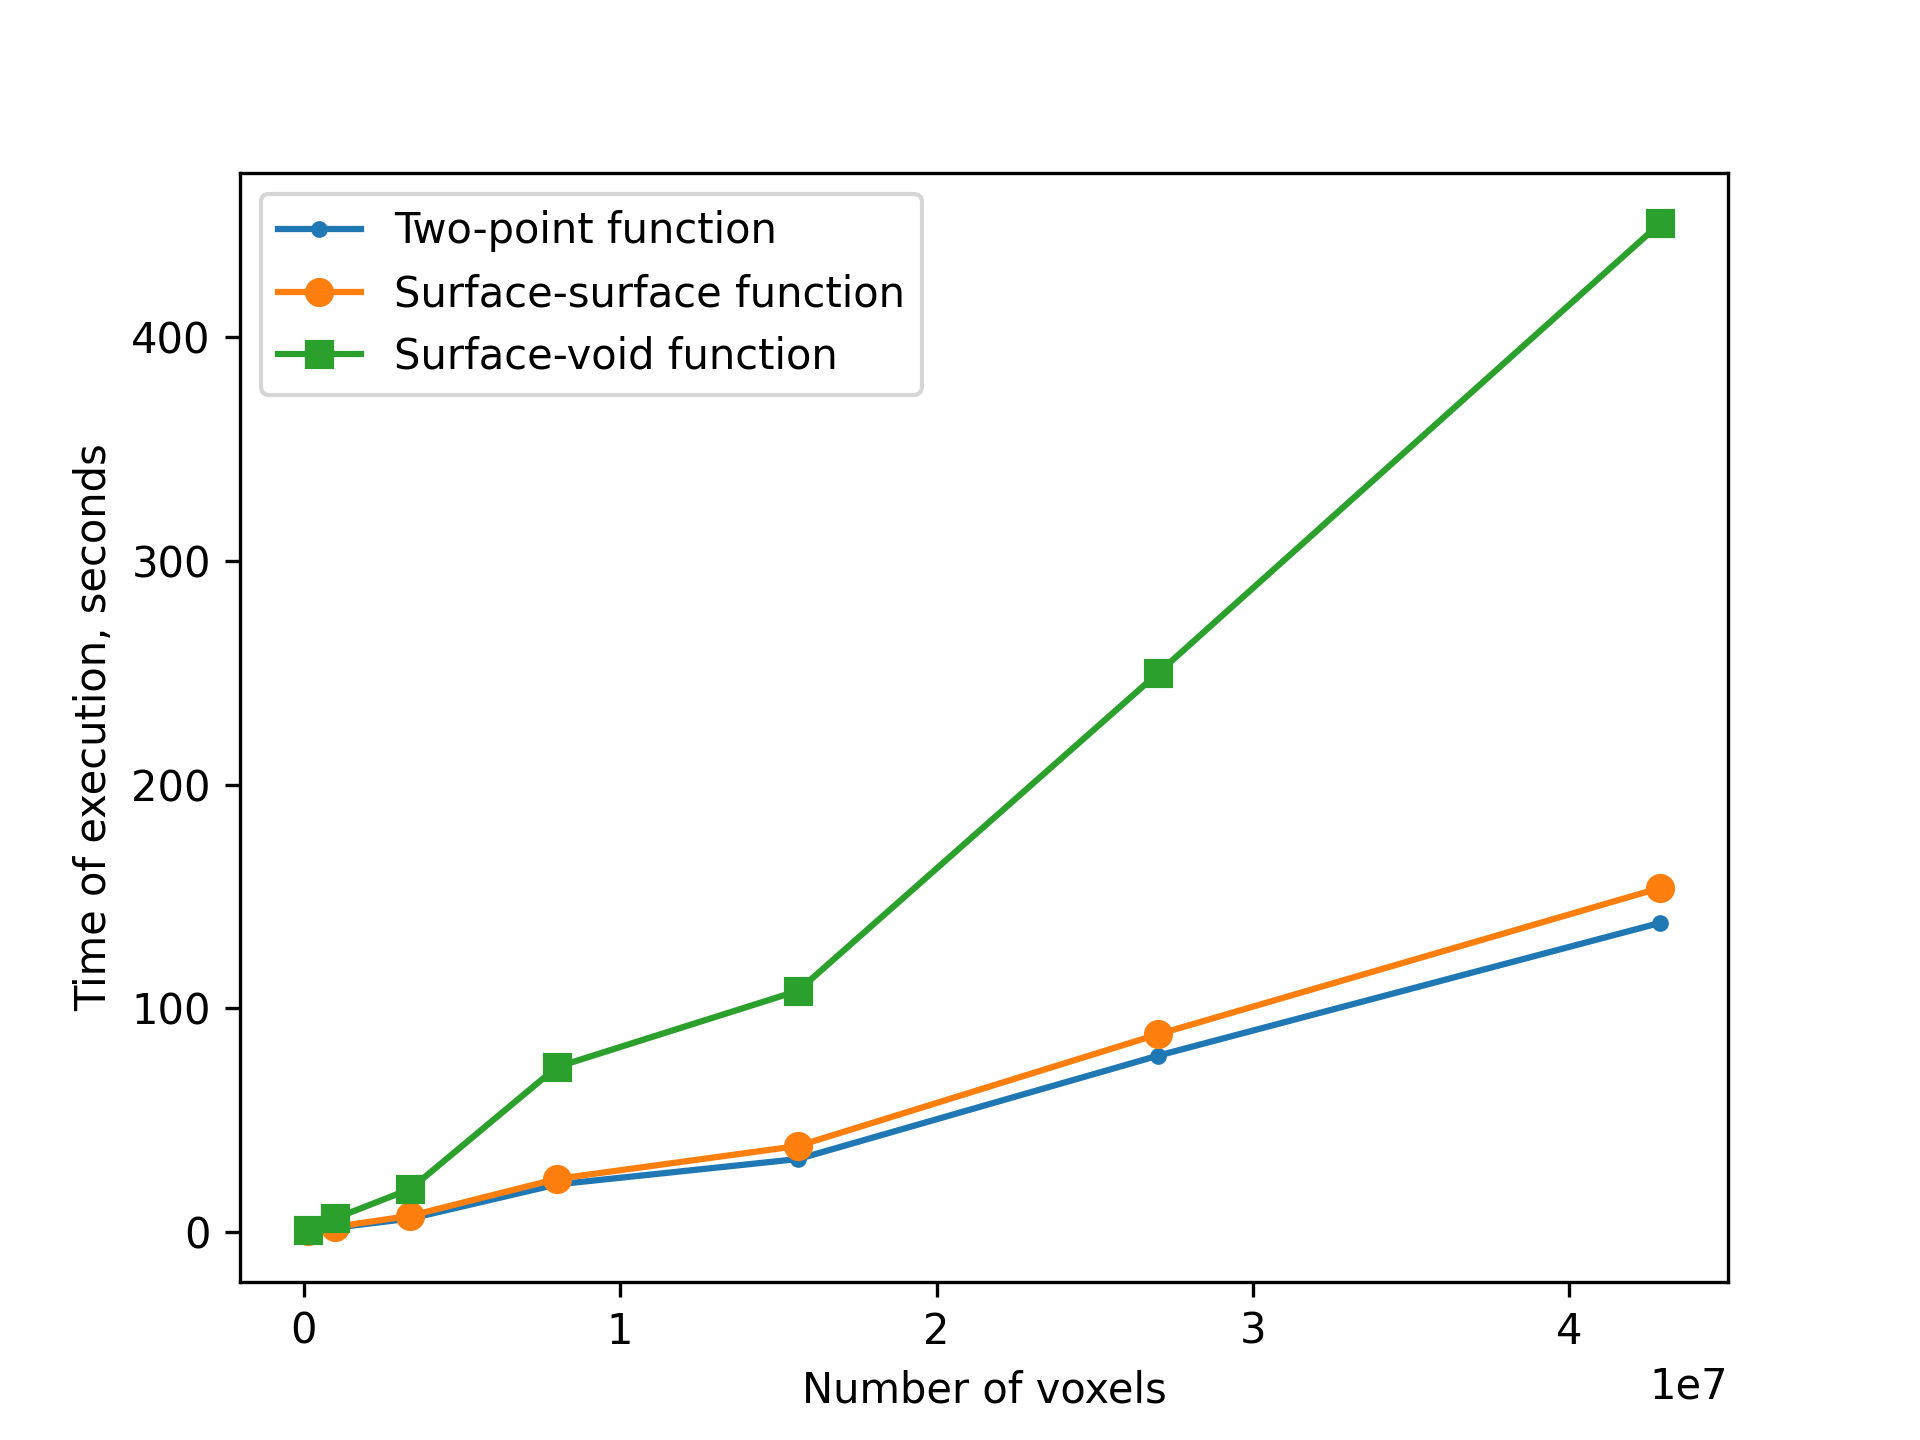
\includegraphics[width=0.475\linewidth]{images/time-3d-map.png}
    \label{fig:timings-3d-map}}
  \vskip\baselineskip
  \subfigure[Two-dimensional case, module \code{Map}, GPU]{
    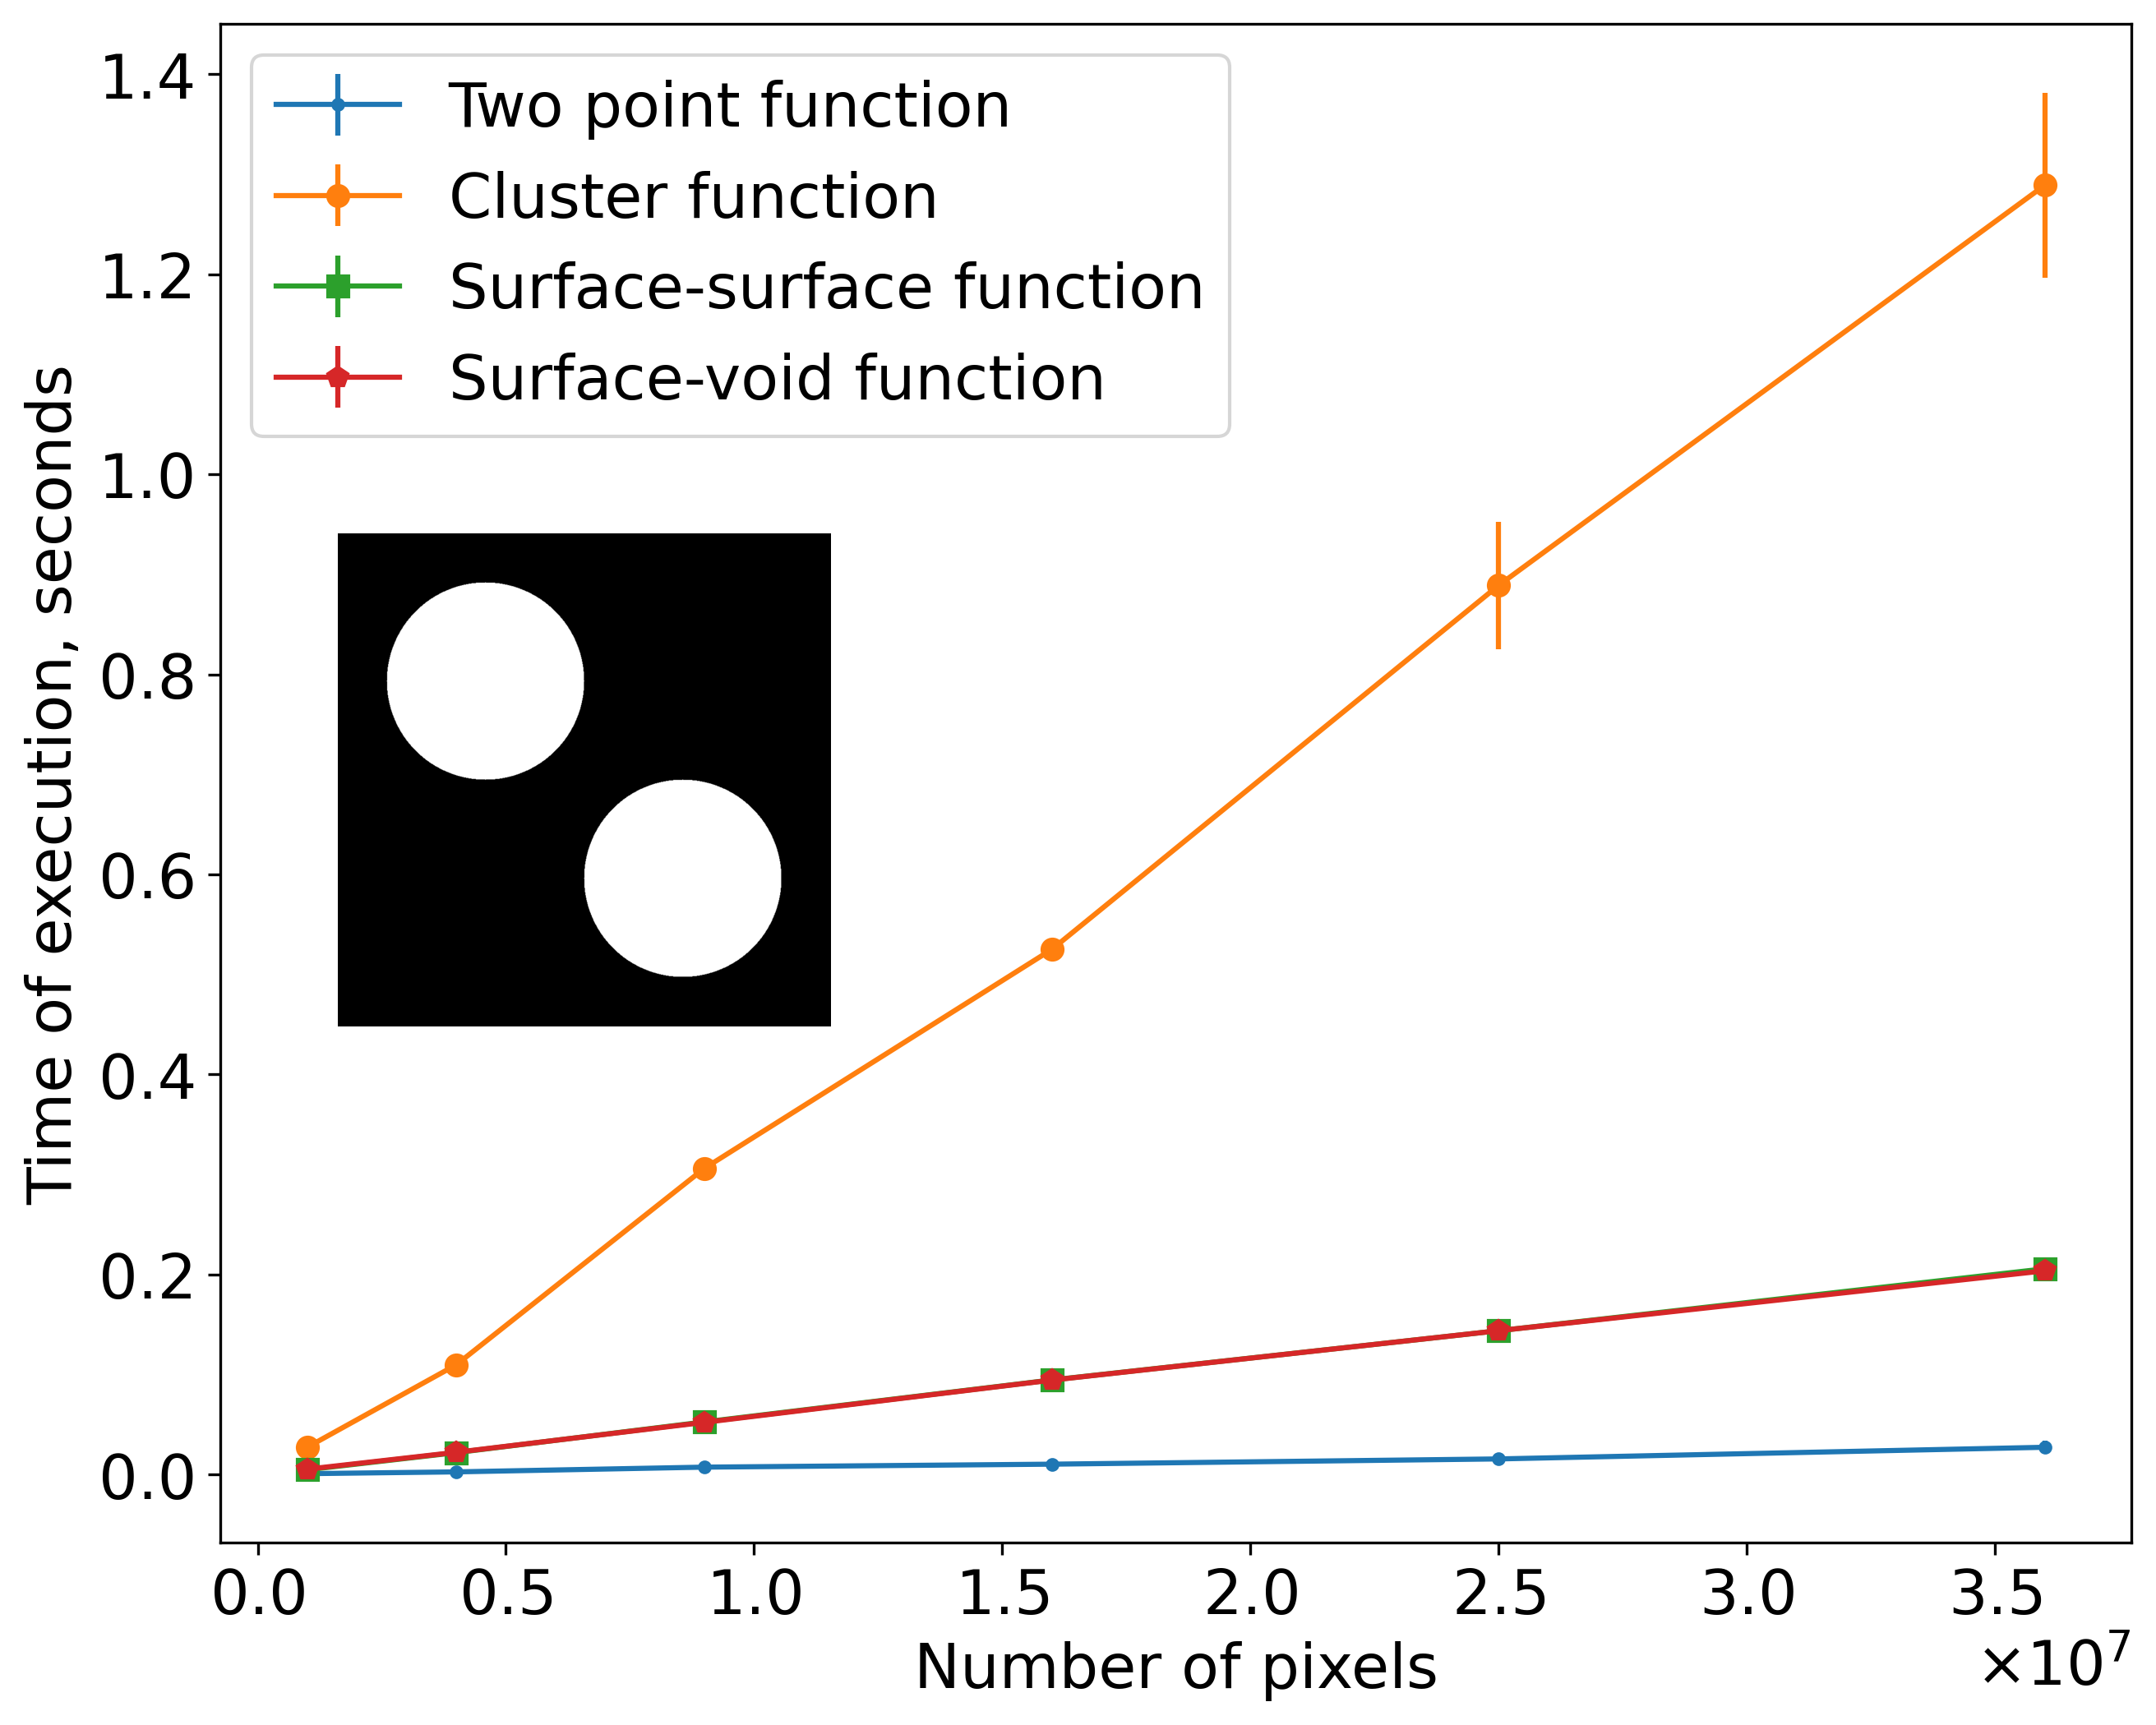
\includegraphics[width=0.475\linewidth]{images/time-2d-gpu.png}
    \label{fig:timings-2d-gpu}}
  \hfill
  \subfigure[Three-dimensional case, module \code{Map}, GPU]{
    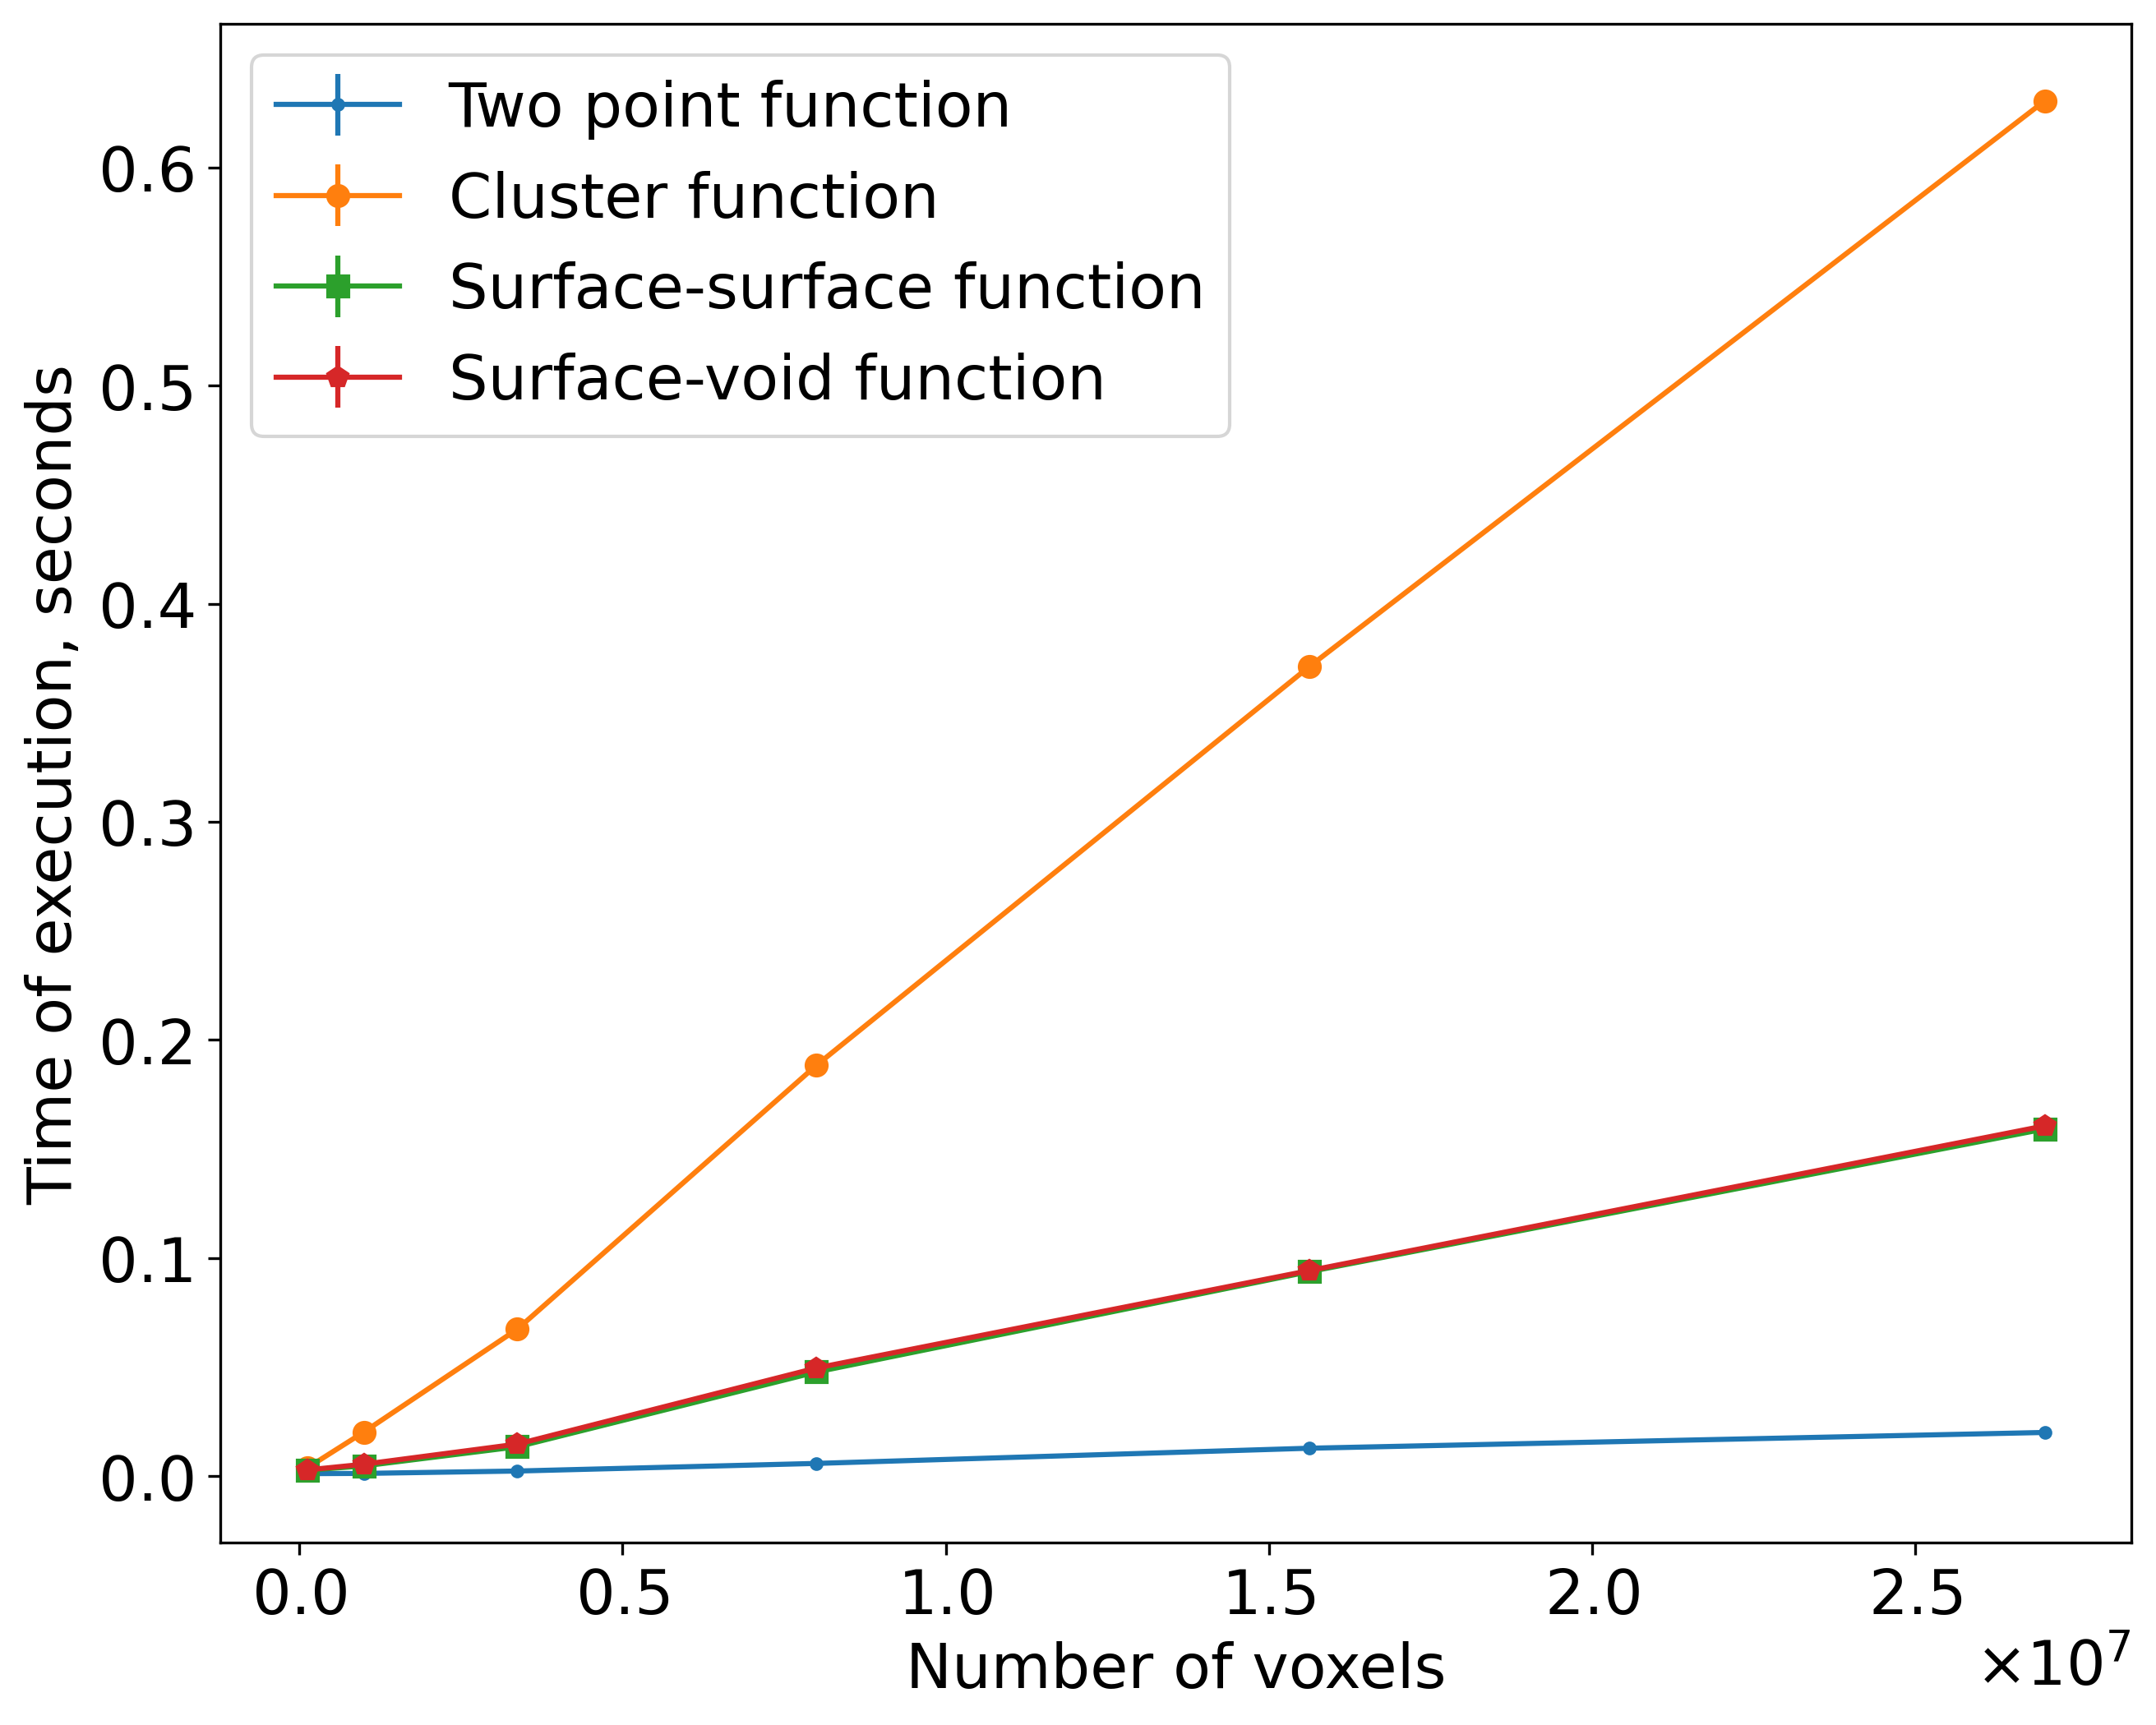
\includegraphics[width=0.475\linewidth]{images/time-3d-gpu.png}
    \label{fig:timings-3d-gpu}}
  \caption[]{Execution times for different correlation functions.}
  \label{fig:timings}
\end{figure*}

\section{Summary}
\label{sec:summary}
Text

\appendix
\section{Computation of number of trials for non-periodic mode}
\label{sec:number-of-trials}
Here we assume that an input is padded with zeros to the length $2s_i - 1$
across each dimension $i$ where $s_i$ is the size of the unpadded input in that
dimension. For each dimension we calculate a sequence
\begin{equation*}
  N^i_j = \left\{
  \begin{array}{cc}
    s_i - j & \quad j \in \overline{0, s_i-1} \\
    j - s_i + 1 & \quad j \in \overline{s_i, 2s_i-2}
  \end{array}
  \right.
\end{equation*}

When a number of trials is calculated as follows:
\begin{equation*}
  N_{i_1, i_2, \dots, i_n} = \prod_{k=1}^n N^k_{i_k}
\end{equation*}
Here $n$ is a number of dimensions and $i_k$ is an index into the output array
for $k$-th dimension.

\bibliography{apssamp}
\end{document}
